%!TEX TS-program = xelatex
\documentclass[10pt,twoside]{article}\usepackage[]{graphicx}\usepackage[]{color}

\usepackage{alltt}
\usepackage{graphicx}
\usepackage{gensymb}
\usepackage[top=1cm, bottom=1.5cm, left=1.2cm, right=1.2cm]{geometry}
\usepackage[font=small]{caption}
\usepackage{adjustbox}
\usepackage{fancyhdr}
\usepackage{layout}
\usepackage{booktabs}
\usepackage{kpfonts}
\usepackage[explicit]{titlesec}
\usepackage{wrapfig}
\usepackage{tcolorbox}
\usepackage{xcolor}
\usepackage{setspace}
\usepackage{parskip}
\usepackage{tikz}
\usepackage{fontspec}
\usepackage{anyfontsize}
%\usepackage[utf8]{inputenc}
%\usepackage[ngerman]{babel}
%\usepackage{newunicodechar}
%\usepackage{lmodern}% http://ctan.org/pkg/lm



\setmainfont{Calibri}

% Headers and Footers
\pagestyle{fancy}
\renewcommand{\headrulewidth}{0pt}
\rhead{}
\lhead{}
\cfoot{}
\fancyfoot[LE,RO]{\thepage}

% Box line thickness setting
\setlength{\fboxrule}{1.5pt}

\setlength{\headsep}{0.2in}

\newcommand*{\ChapterFont}{%
	\fontseries{b}
	\doublespacing
	\fontsize{40}{20}%
	\color{white}
	\pagecolor{2dblue}
	\selectfont}

\newcommand*{\PageHeading}[1]{%
	\begin{tikzpicture}[remember picture,overlay]
		\node[anchor=north west,minimum width=21.6cm,minimum height=2cm,fill=2dblue, font=\bf,align=center,text=white] (RB) at (current page.north west){\Large #1};
	\end{tikzpicture}}


\newcommand*{\SectionHeading}[2]{%
	\begin{tikzpicture}[remember picture,overlay]
	\node[anchor=south west, yshift = 4cm ,minimum width=21.6cm,minimum height=6cm,fill=2dblue, text width=18cm, font=\bf,text=white] (RB) at (current page.south west){\Huge #1};
	\node[anchor=south west, yshift = 2.9cm ,minimum width=21.6cm,minimum height=6cm, text width=18cm, font=\bf,text=white] (RB) at (current page.south west){\Huge #2};
	\end{tikzpicture}}



\setlength{\parskip}{1em}

%Sets size and colour: section titles
\renewcommand{\familydefault}{\sfdefault}
\usepackage{xcolor}
\definecolor{2dblue}{RGB}{8, 70, 101}
\definecolor{backgroundgrey}{RGB}{242,242,242}
%\definecolor{redbox}{RGB}{192,0,0}
%\definecolor{bluebox}{RGB}{33,89,104}
\usepackage{titlesec}
\titleformat{\section}
{\normalfont\Large\centering\bfseries\color{2dblue}}
{\thesection}{1em}{}



\IfFileExists{upquote.sty}{\usepackage{upquote}}{}

\begin{document}

\section*{P1}
	\thispagestyle{empty}
	\pagecolor{2dblue}
	\begin{center}
		
		{\Huge\color{white}{
				\textbf{
					HeadingP01b
				}
				\par
				HeadingP01c}}
		\vspace{2cm}
		
		{\fontsize{20pt}{30pt}\selectfont\color{white}\textbf{FrontPageTitleAddition}\par}
		{\fontsize{16pt}{16pt}\selectfont\color{white}{FrontPageAddition
				
				
				\textbf{FrontPageDate}
			}\par}
		\vspace{1cm}
		
		\adjincludegraphics[height=10cm,trim={0cm 0cm 0cm 0cm},clip]{ReportGraphics/Picture1}	
		
\end{center}
\begin{tikzpicture}[remember picture,overlay]
\node[anchor=south west, yshift = 0cm ,minimum width=21.6cm,minimum height=4cm,fill=white] (RB) at (current page.south west){
	\adjincludegraphics[height=2.8cm,trim={0cm 0cm 0cm 0cm},clip]{ReportGraphics/Logo_front}
	\hspace{3.5cm}
	\adjincludegraphics[height=2.8cm,trim={0cm 0cm 0cm 0cm},clip]{ReportGraphics/PACTA_Logo}};
\end{tikzpicture}

\newpage
\pagecolor{white}		
\section*{P2} % 1st Section
\thispagestyle{empty}
\vspace{17cm}
\SectionHeading{Section01:}{SectionTitle01}

\newpage
\singlespacing
\normalfont
\pagecolor{white}
\color{black}

\newpage
\section*{P3}
\PageHeading{HeadingP03}

\textbf{AddPage1text}

ContentP03


\newpage
\section*{P4} % Into to portfolio
\PageHeading{HeadingP4}


\begin{wrapfigure}{r}{0.5\linewidth}
	\vspace{-.3cm}
	\textbf{CaptionP4a
	}
	\newline
	\vspace{-.6cm}
	\center{\adjincludegraphics[width = 1\linewidth,trim={0cm 0cm 0cm 0cm},clip]{SwissFigures/Fig00}	}
	\vspace{-2.2cm}
	\newline

\end{wrapfigure}

ContentP4

\vspace{.5cm}

\begin{minipage}[t]{.48\textwidth}	%EQPieS
\fcolorbox{black}{white}{ 
	\parbox{1\linewidth}{
		\centering
	\textbf{CaptionP4b} \newline
	\textbf{EQCoverage} CaptionP4d \newline
	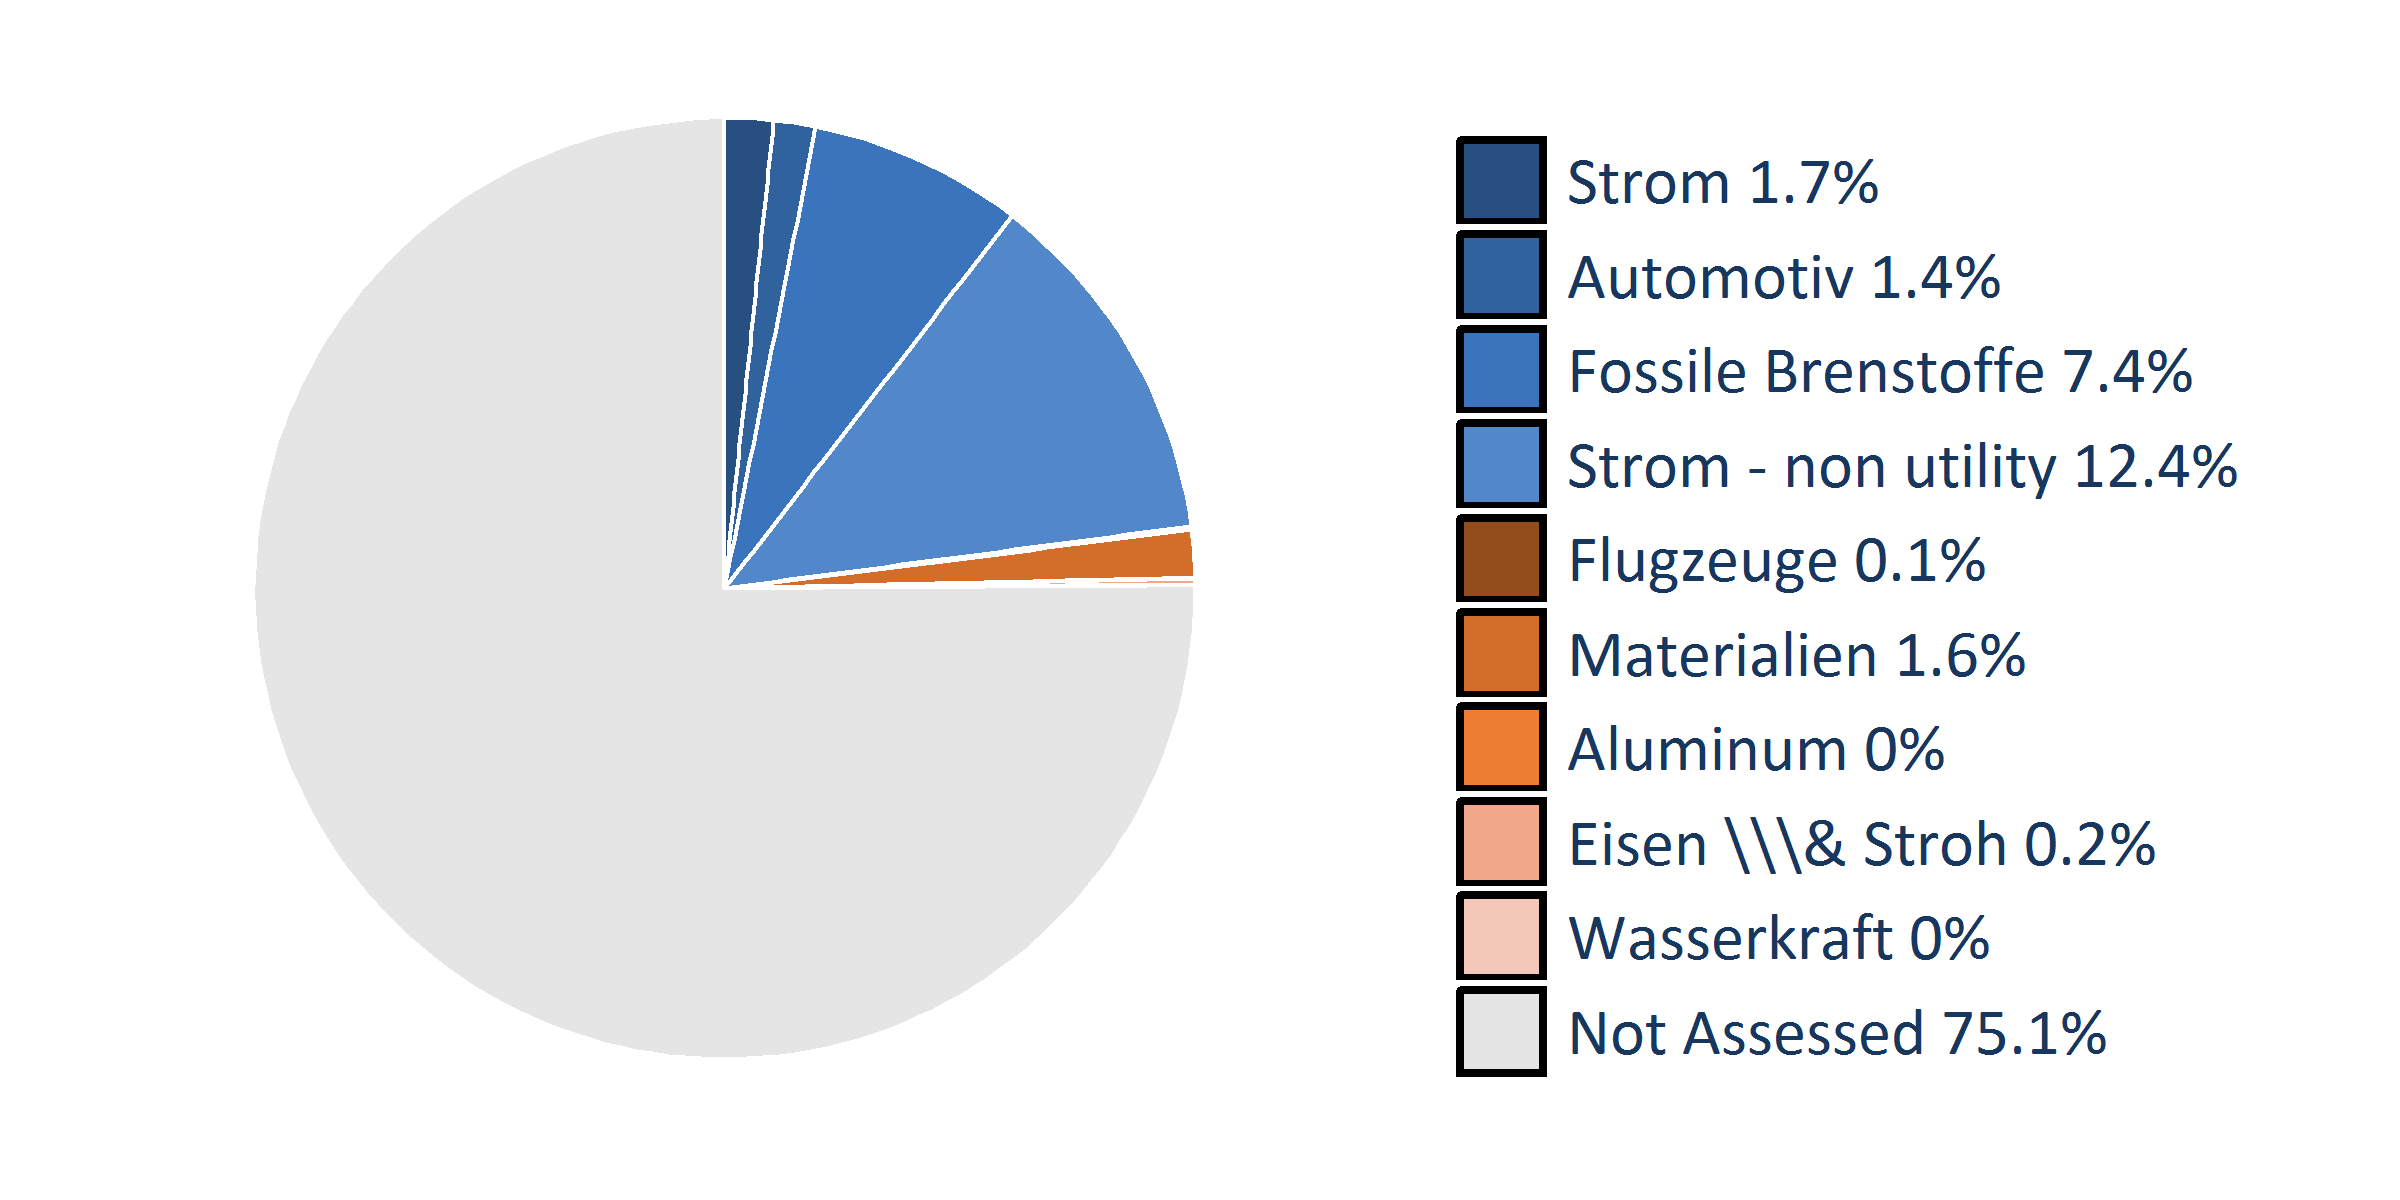
\includegraphics[width=1\linewidth]{SwissFigures/Fig01}}
}
\end{minipage}
\hspace{.5cm} %EQPieE
\begin{minipage}[t]{.48\textwidth} %CBPieS
\fcolorbox{black}{white}{ 
	\parbox{1\linewidth}{
		\centering
		\textbf{CaptionP4c} \newline
		\textbf{CBCoverage} CaptionP4d \newline
		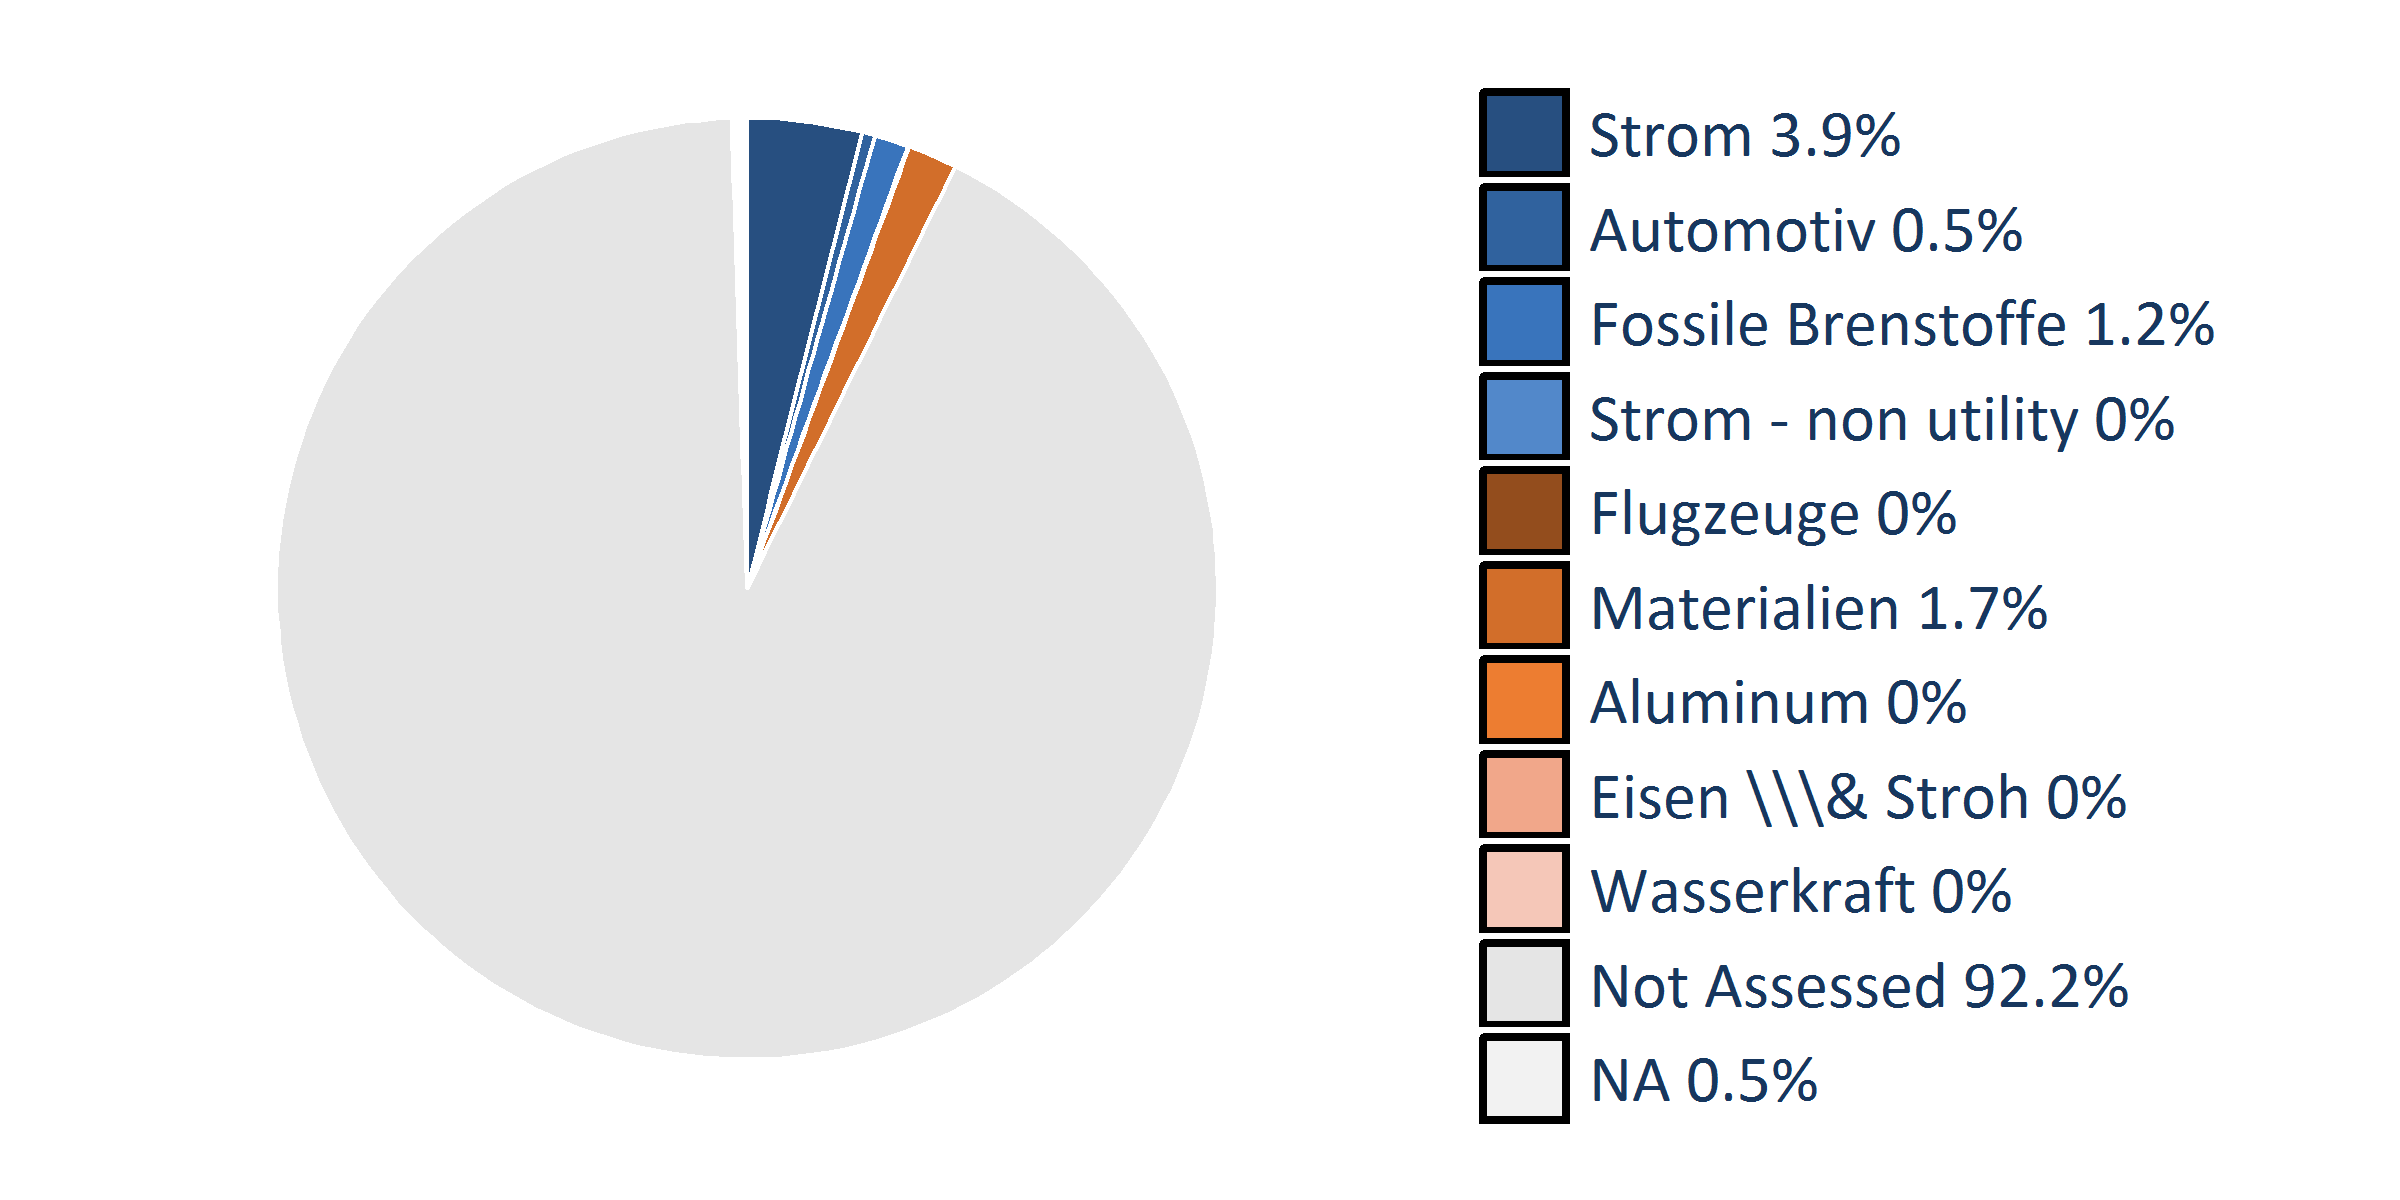
\includegraphics[width=1\linewidth]{SwissFigures/Fig02}}
}
\end{minipage} %CBPieE

\textit{\small SourceBBG}

\newpage
\section*{P5} % Background a
\PageHeading{HeadingP5}

\begin{wrapfigure}{t}{0.5\linewidth}
	\vspace{-.45cm}
	\textbf{CaptionP5}
	\center{\includegraphics[trim={0 0cm 0 0 },clip,width=.8\linewidth]{ReportGraphics/FigureP4a_Languagechoose}}
	\vspace{-1.4cm}
\end{wrapfigure}

ContentP5

{\centering\includegraphics[trim={0 .6cm 0 1.2cm},clip,width=.8\linewidth]{ReportGraphics/FigureP4b_Languagechoose}\par}

\newpage
\section*{P05} % Background b
\PageHeading{HeadingP05a}

\textbf{HeadingP05b}

ContentP05b

\begin{itemize}
	\item ListP05a
	\item ListP05b
	\item ListP05c
\end{itemize}

\textbf{HeadingP05c}

ContentP05c

\textbf{HeadingP05d}

ContentP05d

\textbf{HeadingP05e}

ContentP05e
\begin{itemize}
	\item ListP05d
	\item The model takes a diversified ‘market portfolio’ as a basis, focusing on key technologies reflected in the IEListP05e  	
\end{itemize}	


\newpage
\section{P005} % Feedback on the model
\PageHeading{HeadingP005a}


ContentP005b 

\begin{itemize}
\item \textbf{ListP005a} ListP005b
\item \textbf{ListP005c} ListP005d
\end{itemize}

ContentP005c

\begin{minipage}[t]{.48\linewidth}
	\centering \textit{ContentP005d}
	
	\includegraphics[trim={0 0 0 0cm},clip,width=1\linewidth]{ReportGraphics/Figure_Feedback_a_Languagechoose}
\end{minipage}
\hspace{.02\linewidth}
\begin{minipage}[t]{.48\linewidth}
	\centering \textit{ContentP005e}
	
	\includegraphics[trim={0 0 0 0},clip,width=1\linewidth]{ReportGraphics/Figure_Feedback_b_Languagechoose}
\end{minipage}

 \newpage
\section*{P06} % FAQ
\PageHeading{HeadingP06}
 
\textbf{FAQQ01} \newline
\textit{FAQA01}

\textbf{FAQQ02} \newline
\textit{FAQA02}

\textbf{FAQQ03} \newline
\textit{FAQA03}

\textbf{FAQQ04} \newline
\textit{FAQA04}

\textbf{FAQQ05} \newline
\textit{FAQA05}

\textbf{FAQQ06} \newline
\textit{FAQA06}

\textbf{FAQQ07} \newline
\textit{FAQA07}

\textbf{FAQQ08} \newline
\textit{FAQA08}

 
\newpage
\section*{P6}
\PageHeading{HeadingP6}

ContentP6

\includegraphics[width=1\linewidth,trim={0 0cm 0 0},clip]{ReportGraphics/FigureP5_Languagechoose}
\newpage
\section*{P7} % 2nd Section
\thispagestyle{empty}
\vspace{17cm}
\SectionHeading{Section02:}{SectionTitle02}


\newpage
\singlespacing
\normalfont
\pagecolor{white}
\color{black}

\newpage
\section*{P8} 		% PowerEQS   EQPageS
\PageHeading{HeadingP8}

ContentP8

\fcolorbox{black}{white}{ 	
	\parbox{1\linewidth}{
	ContentTech1
	
	\vspace{0cm}
	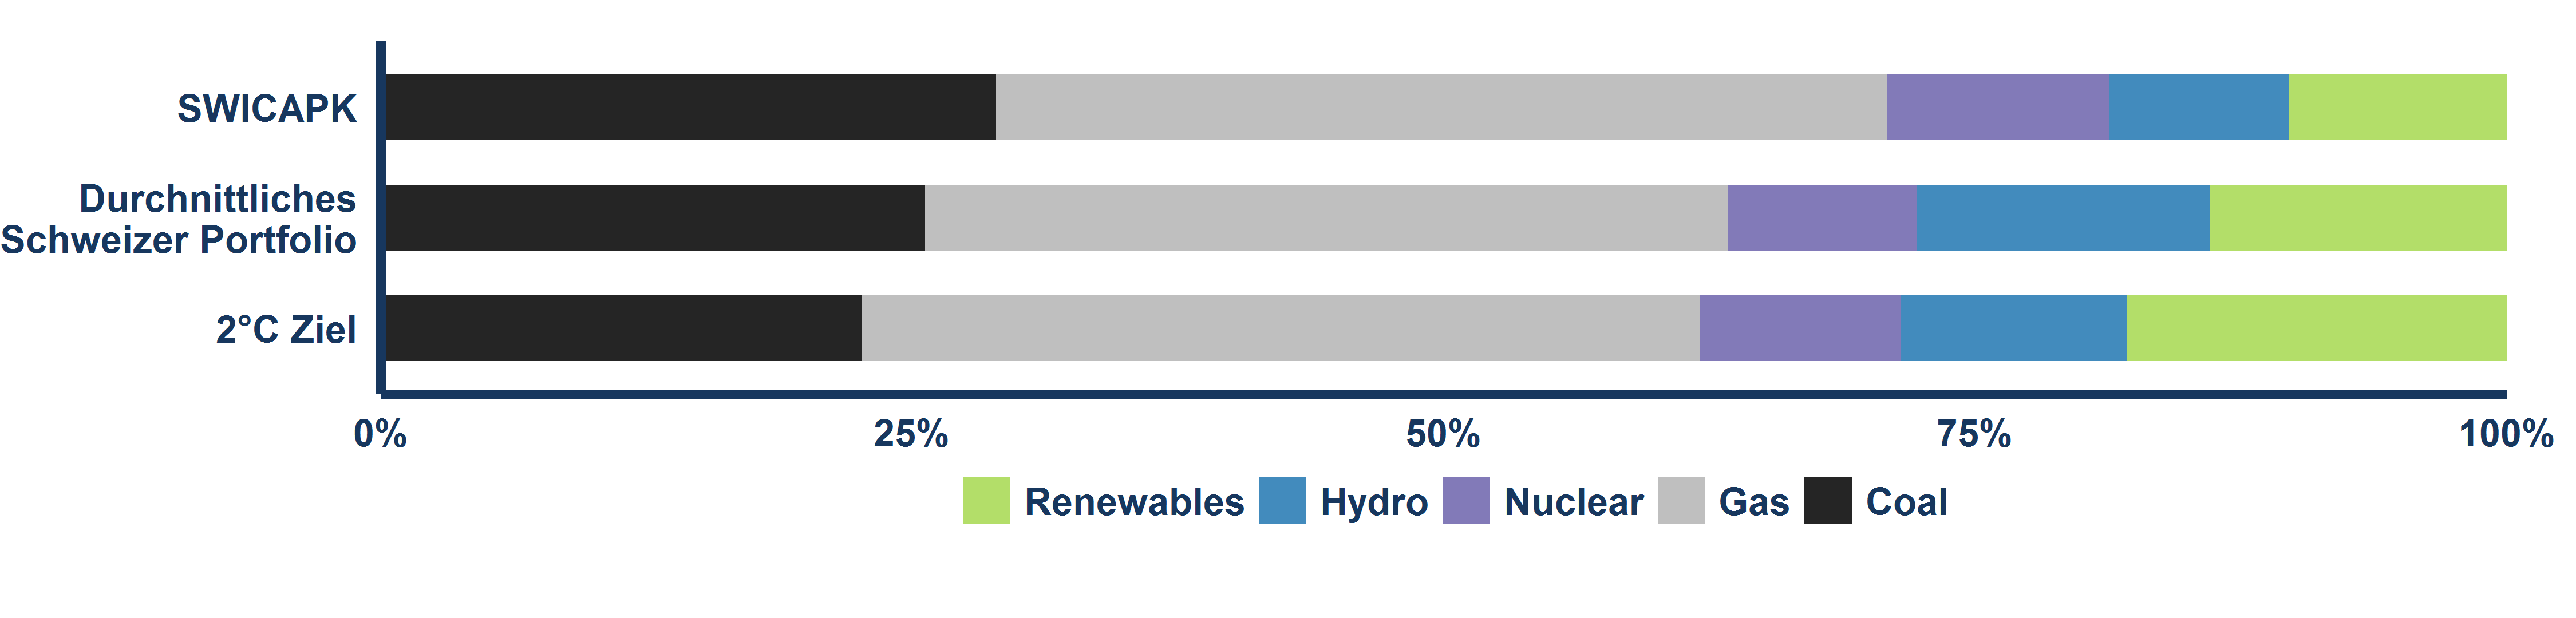
\includegraphics[trim={0 .7cm 0 0},clip,width=1\linewidth]{SwissFigures/Fig03}
	\vspace{-0.5cm}
	\newline
	\begin{minipage}[t]{.32\linewidth}
		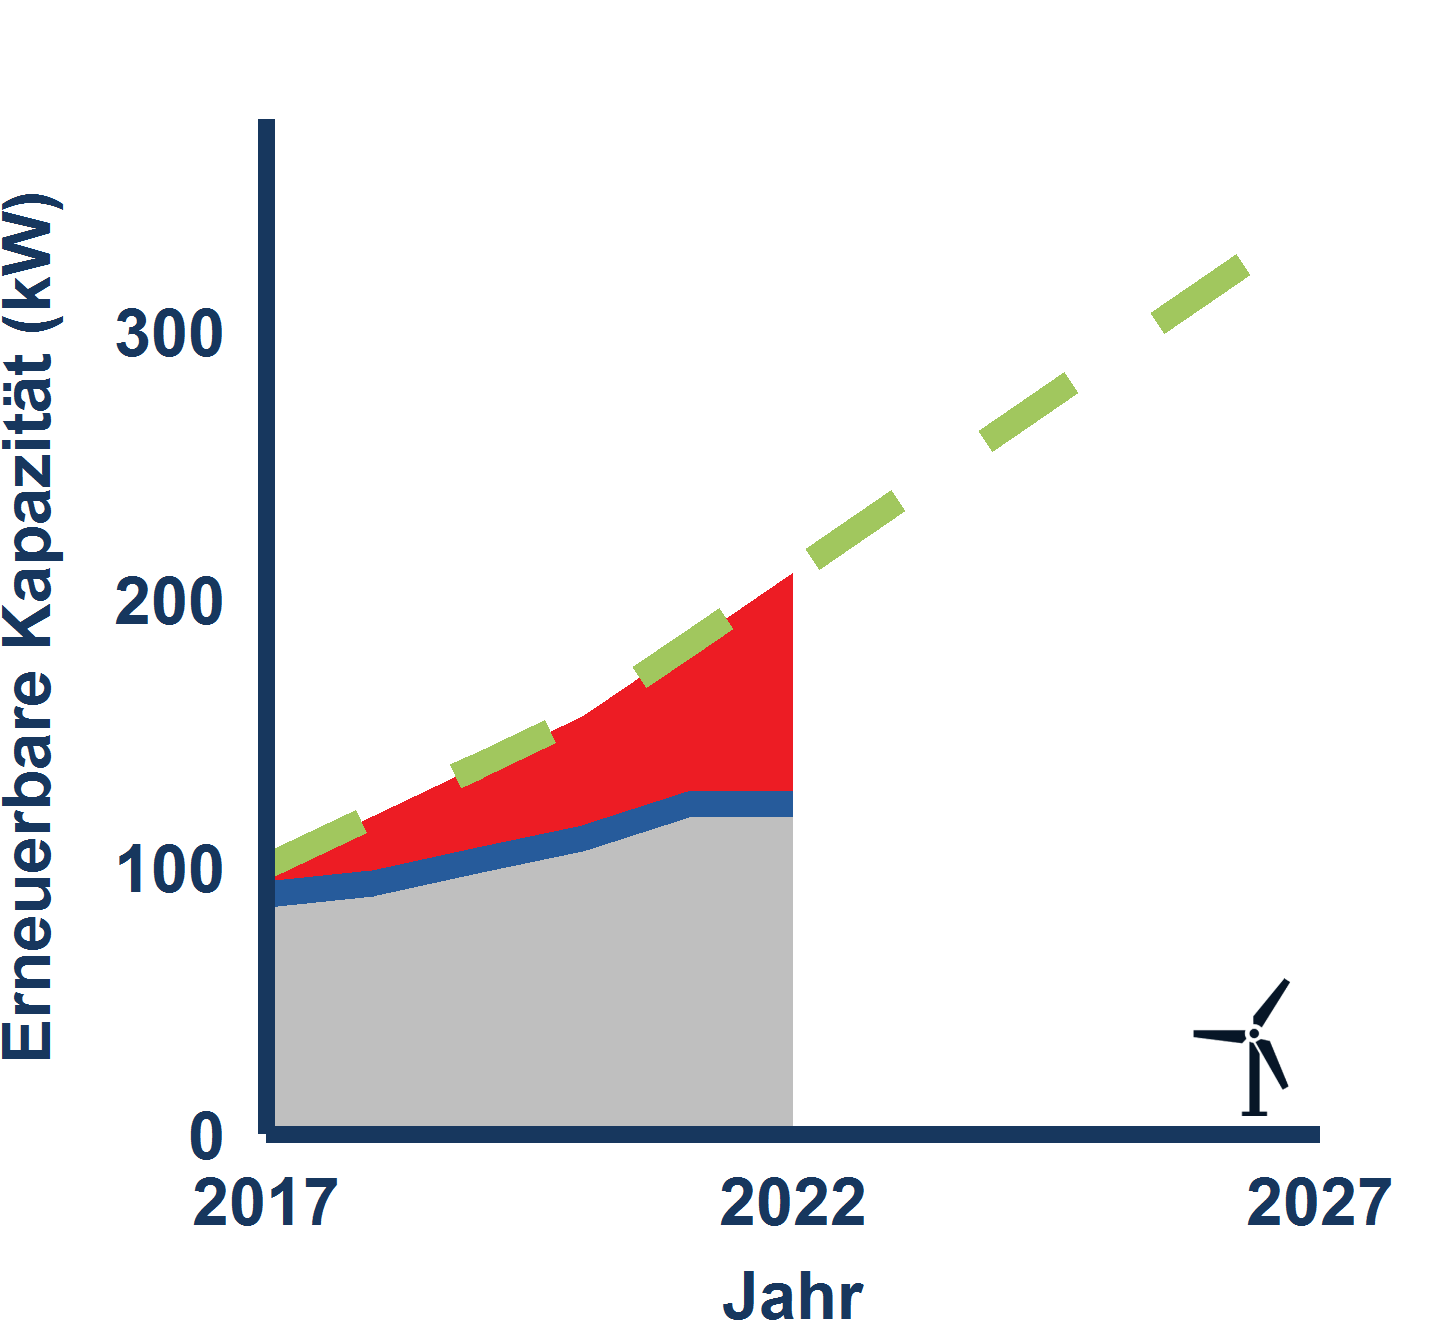
\includegraphics[trim = {0 0cm 0 0},width=1\linewidth]{SwissFigures/Fig04}
		\textbf{CaptionWeight TechRenewablesCap EQCaptionRenewablesCap} %RenewablesCapEQCaption
	\end{minipage}	
		\hspace{.01\linewidth}
	\begin{minipage}[t]{.32\textwidth}
		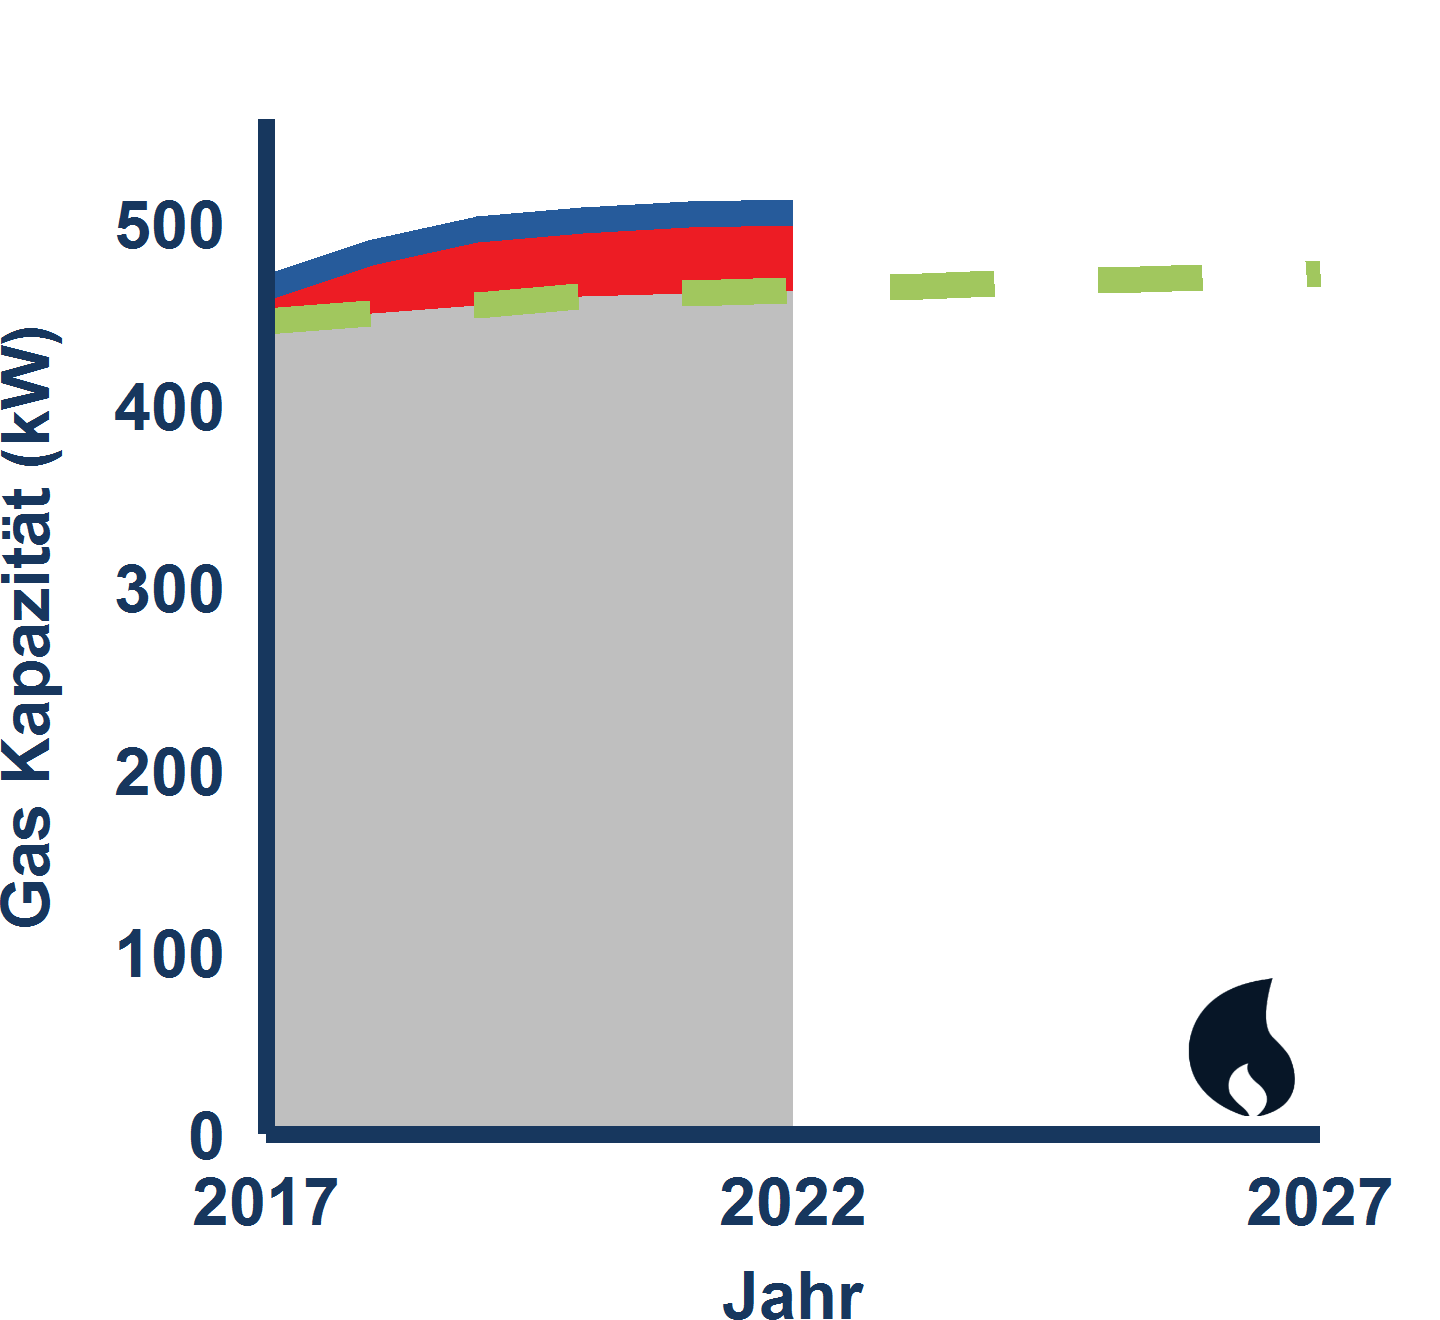
\includegraphics[trim = {0 0cm 0 0},width=1\linewidth]{SwissFigures/Fig06}	
		\textbf{CaptionWeight TechGasCap EQCaptionGasCap} %GasCapEQCaption
	\end{minipage}
		\hspace{.01\linewidth}
	\begin{minipage}[t]{.32\linewidth}
		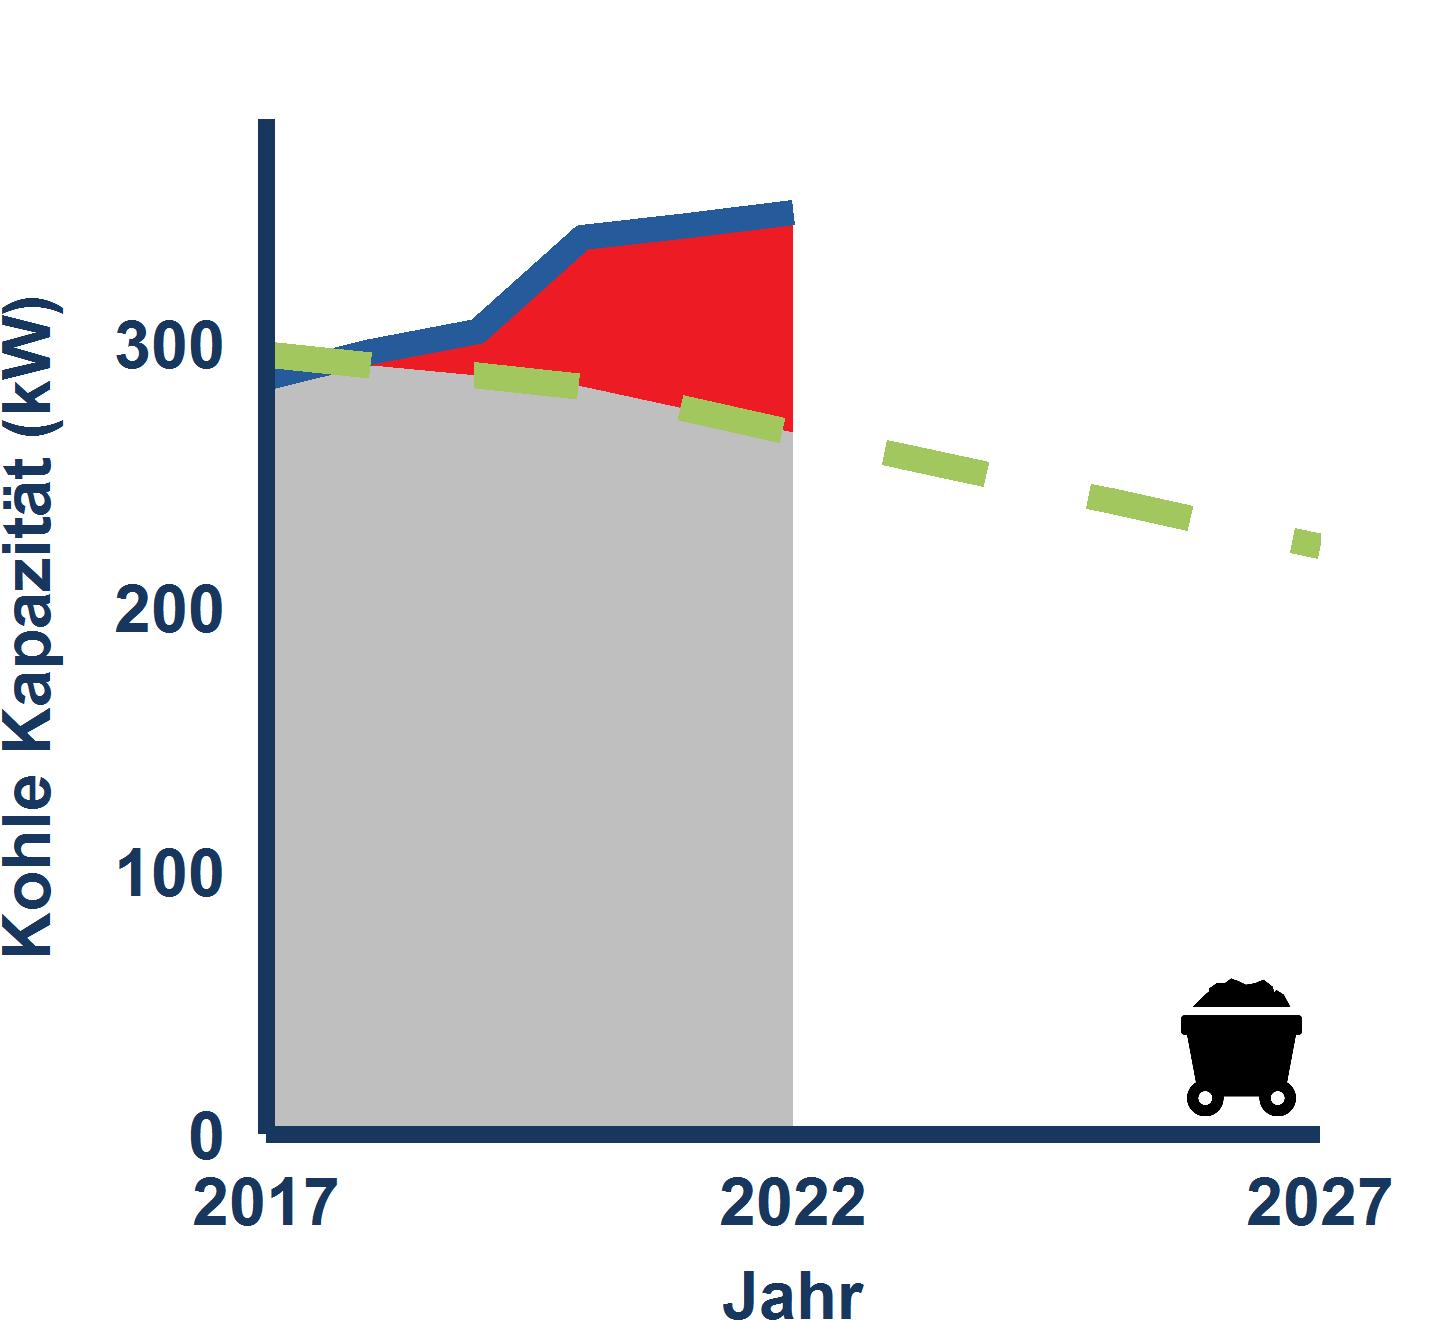
\includegraphics[trim = {0 0cm 0 0},width=1\linewidth]{SwissFigures/Fig05}
		\textbf{CaptionWeight TechCoalCap EQCaptionCoalCap} %CoalCapEQCaption
	\end{minipage}		
	
	{\centering\includegraphics[trim={0 .3cm 0 0.3cm},clip,width=.6\linewidth]{ReportGraphics/LineChartLegend_Languagechoose}\par}

}}

ContentTech2

\fbox{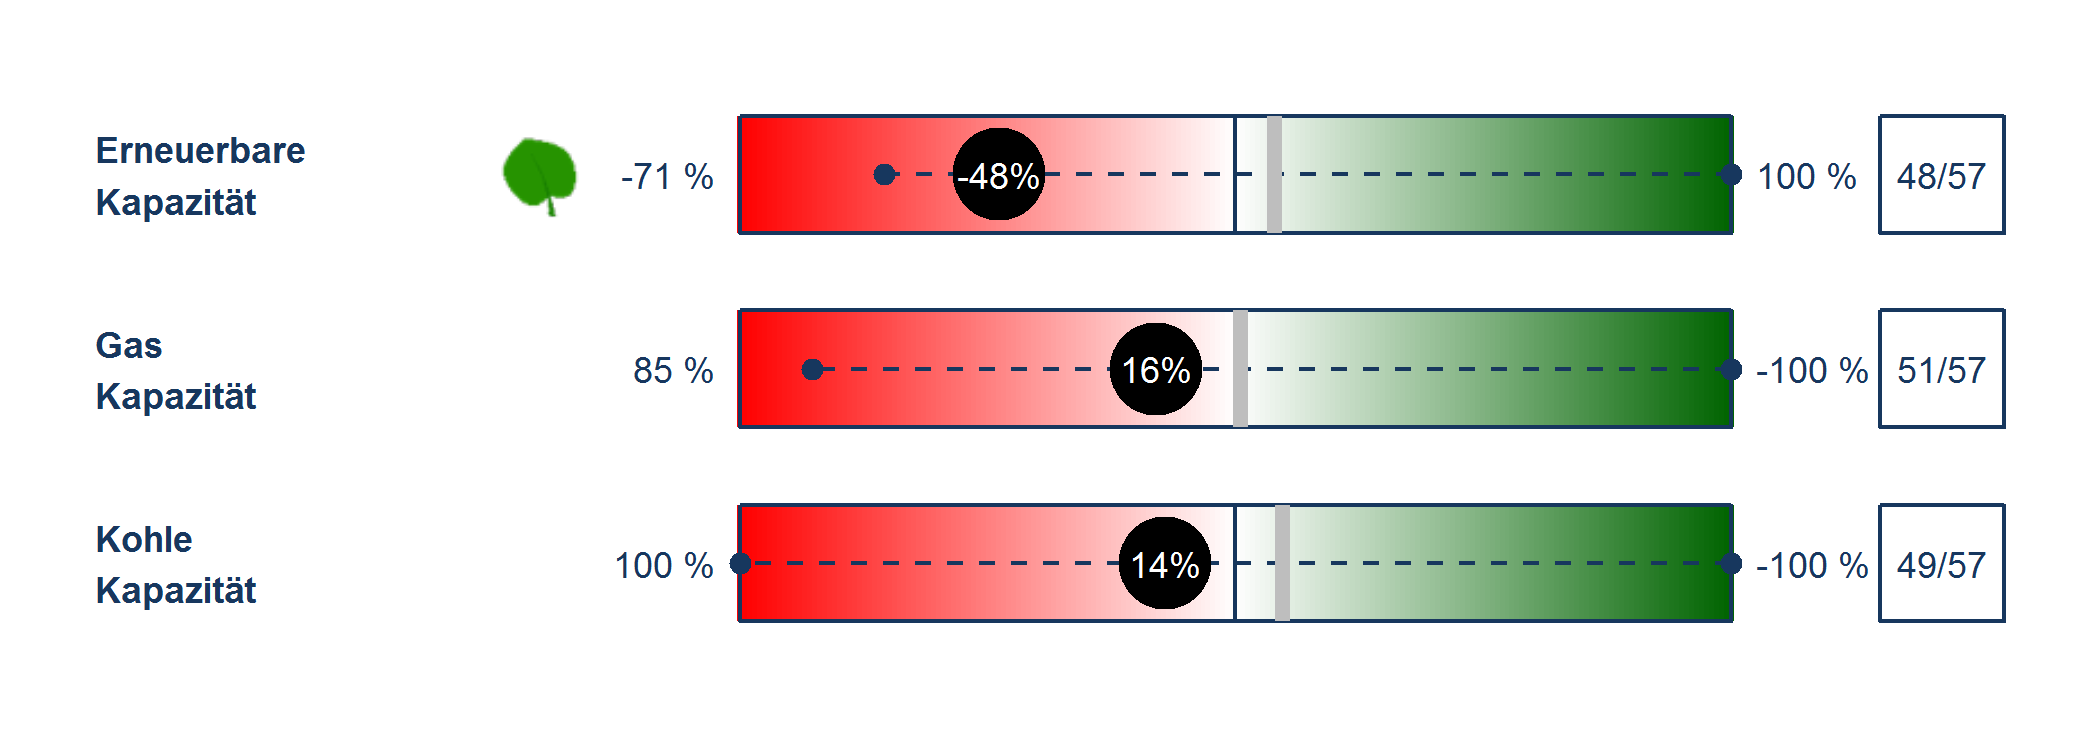
\includegraphics[trim={0 0.9cm 0 0.8cm},clip,width=1\linewidth]{SwissFigures/Fig07}}

\textit{\small SourcePowerFF}

\newpage % PowerEQE EQPageE
\section*{P9} 		% PowerCBS   CBPageS
\PageHeading{HeadingP9}

ContentP9

\fcolorbox{black}{white}{ 	
	\parbox{1\linewidth}{
		ContentTech1
		
		\vspace{0cm}
		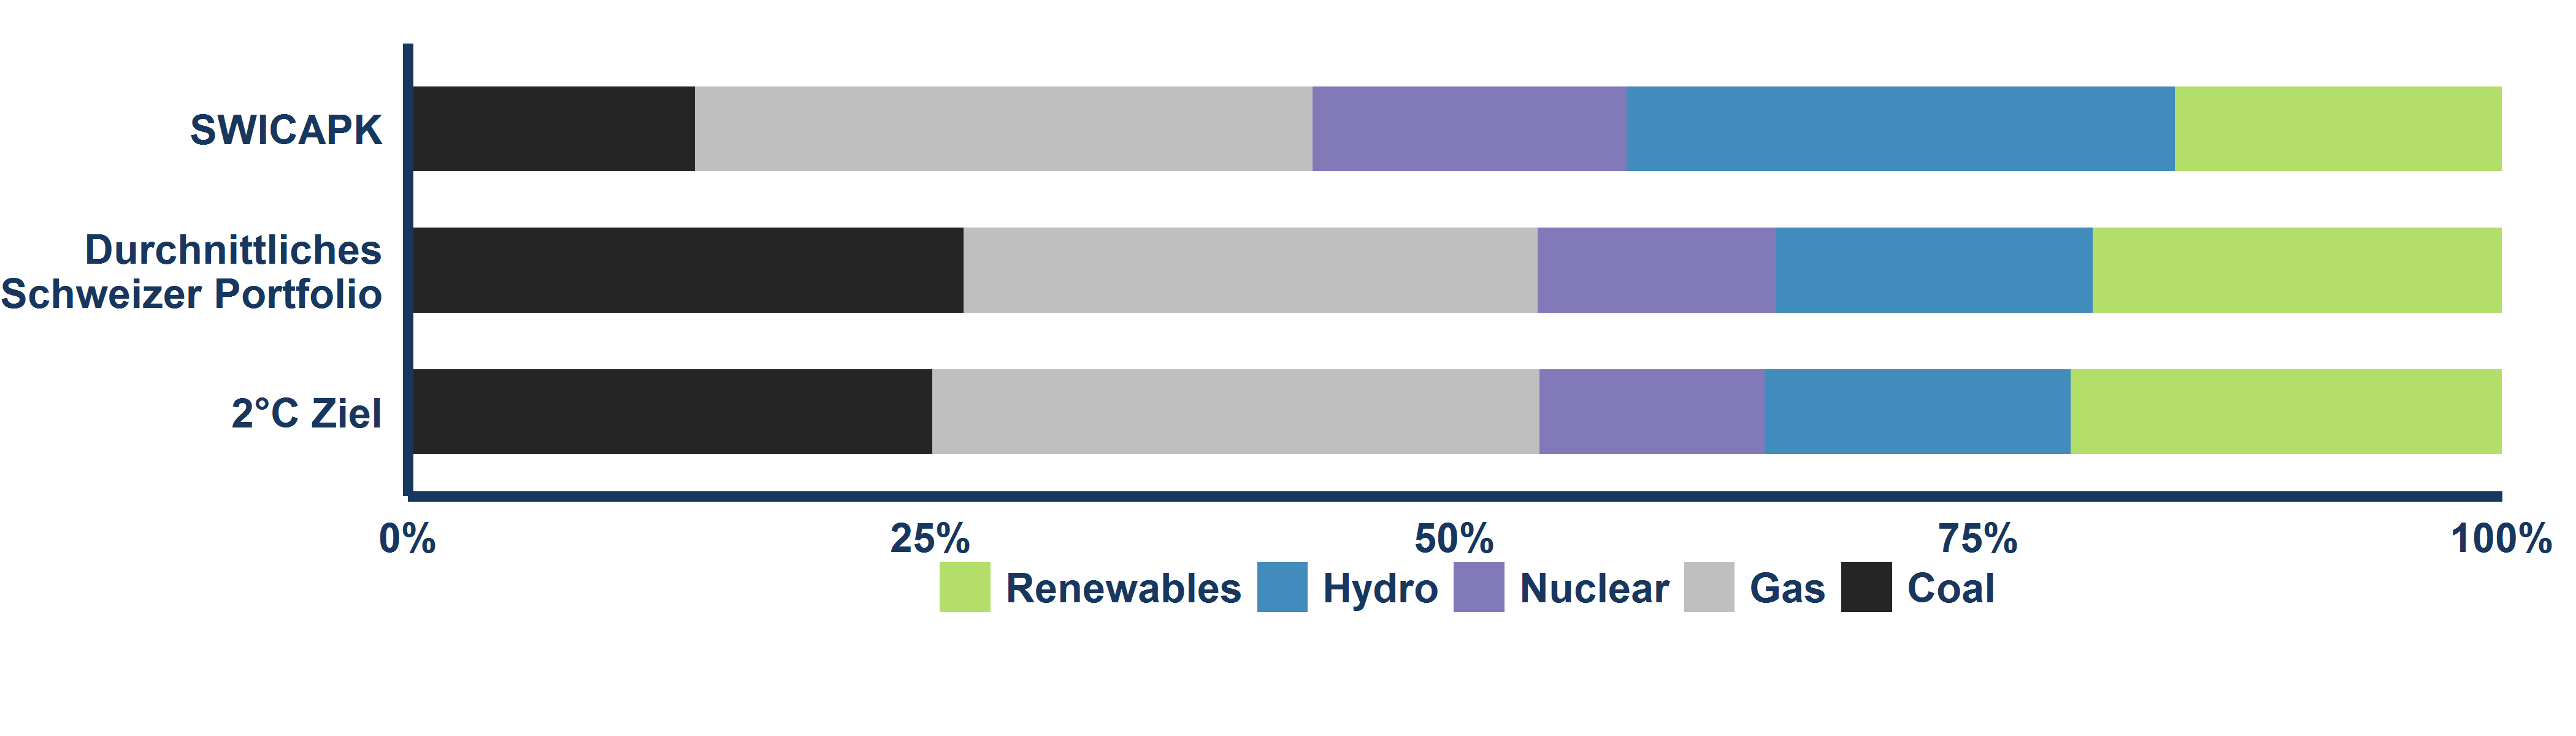
\includegraphics[trim={0 .7cm 0 0},clip,width=1\linewidth]{SwissFigures/Fig08}
		\vspace{-0.5cm}
		\newline
		\begin{minipage}[t]{.32\linewidth}
			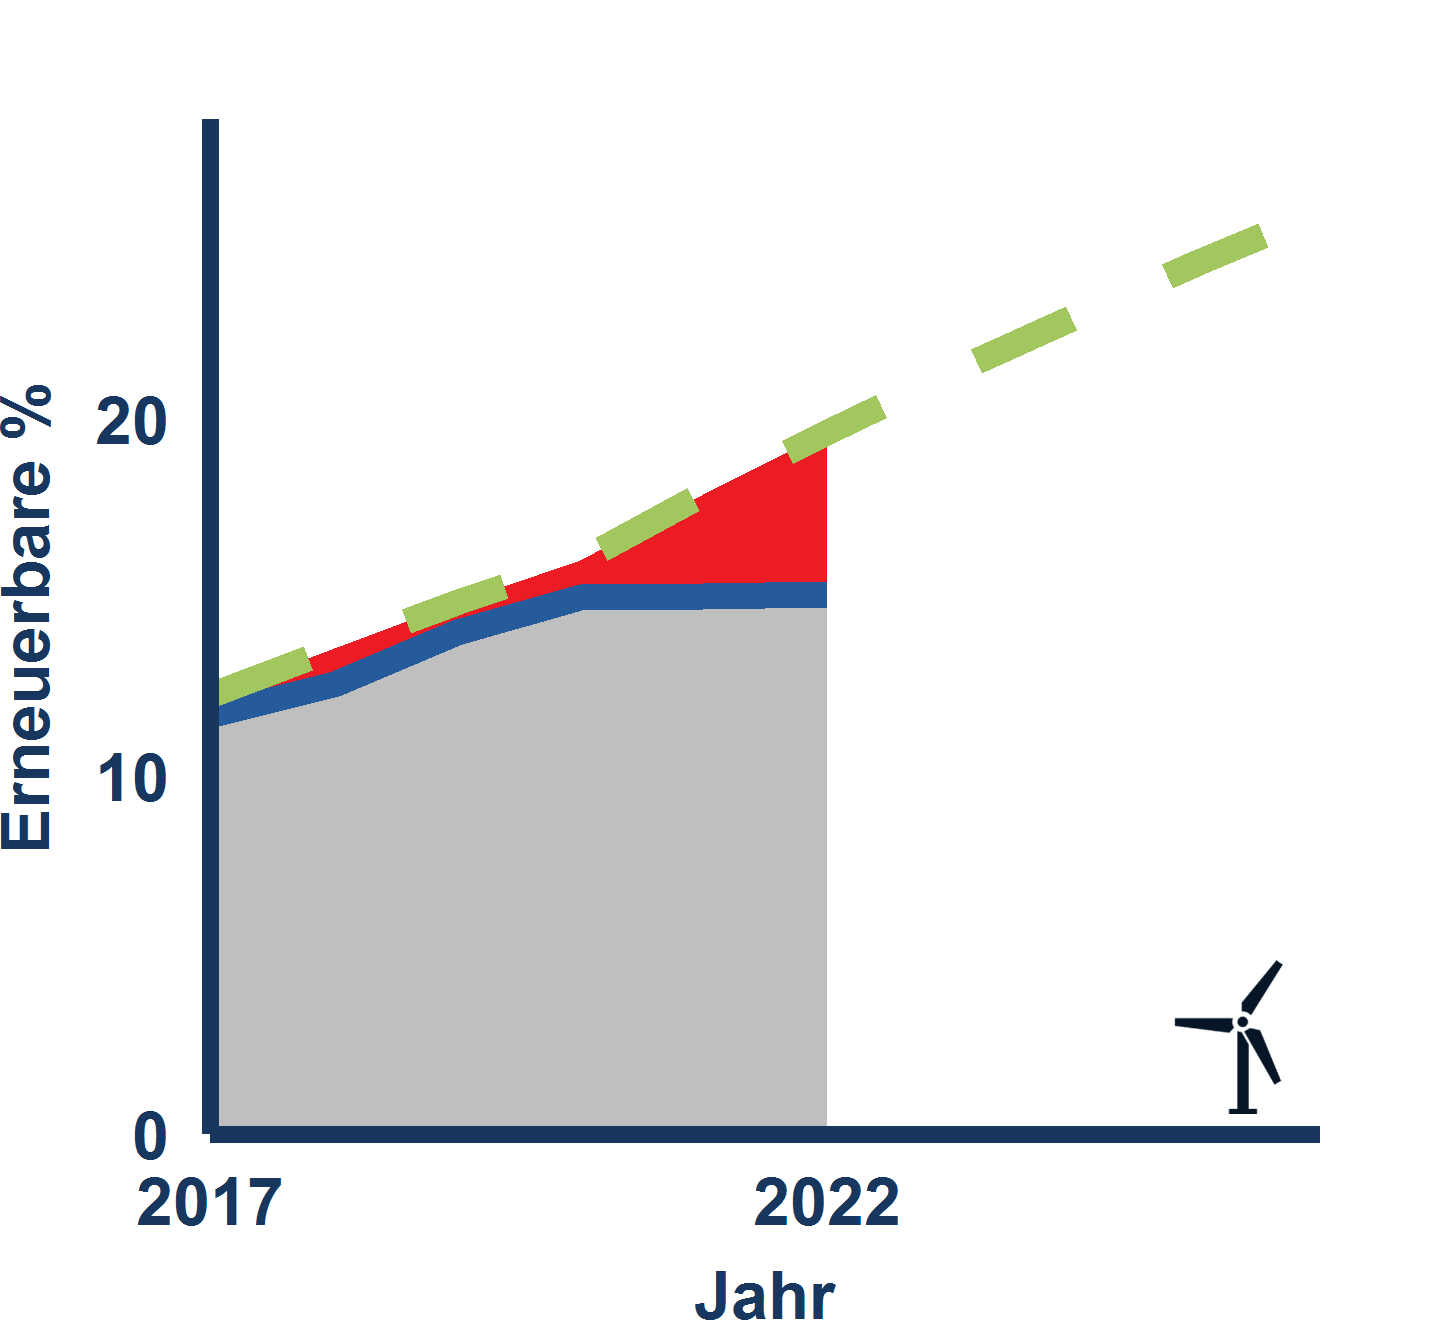
\includegraphics[trim = {0 0cm 0 0},width=1\linewidth]{SwissFigures/Fig09}
			\textbf{CaptionWeight TechRenewablesCap CBCaptionRenewablesCap} %RenewablesCapCBCaption
		\end{minipage}	
		\hspace{.01\linewidth}
		\begin{minipage}[t]{.32\textwidth}
			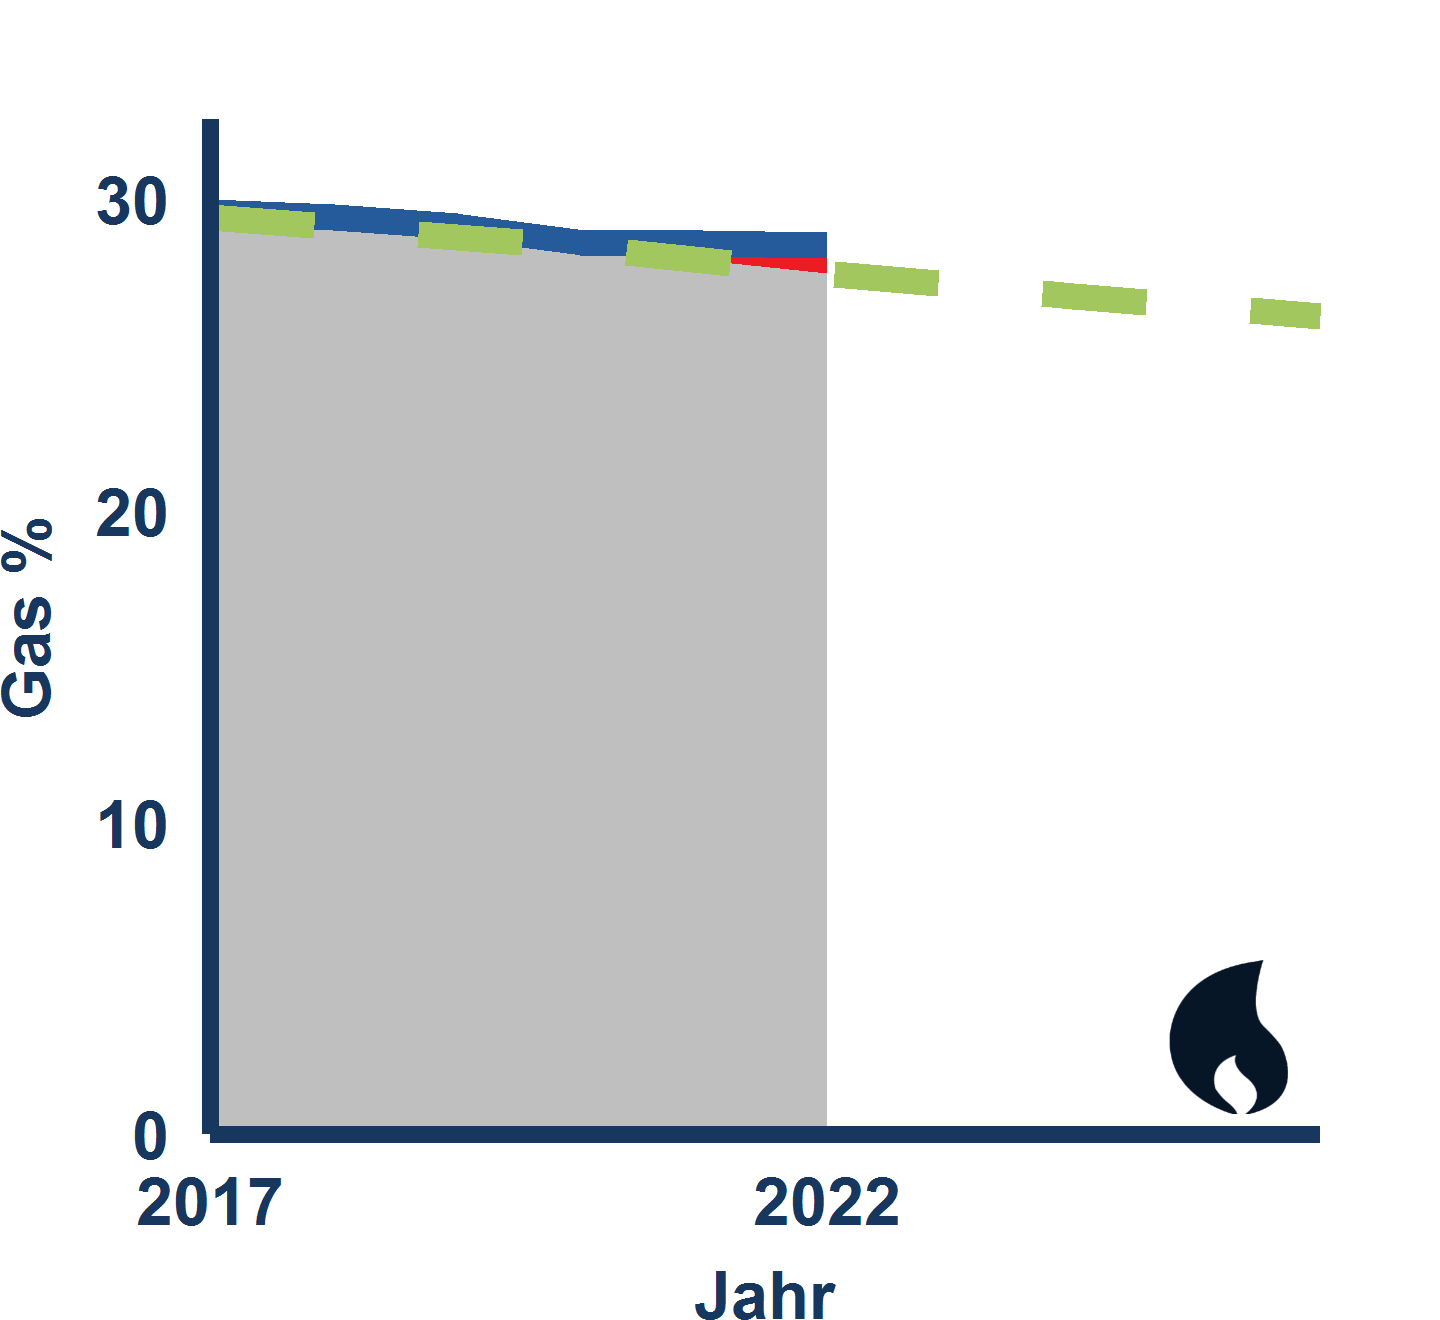
\includegraphics[trim = {0 0cm 0 0},width=1\linewidth]{SwissFigures/Fig11}	
			\textbf{CaptionWeight TechGasCap CBCaptionGasCap} %GasCapCBCaption

		\end{minipage}
		\hspace{.01\linewidth}
		\begin{minipage}[t]{.32\linewidth}
			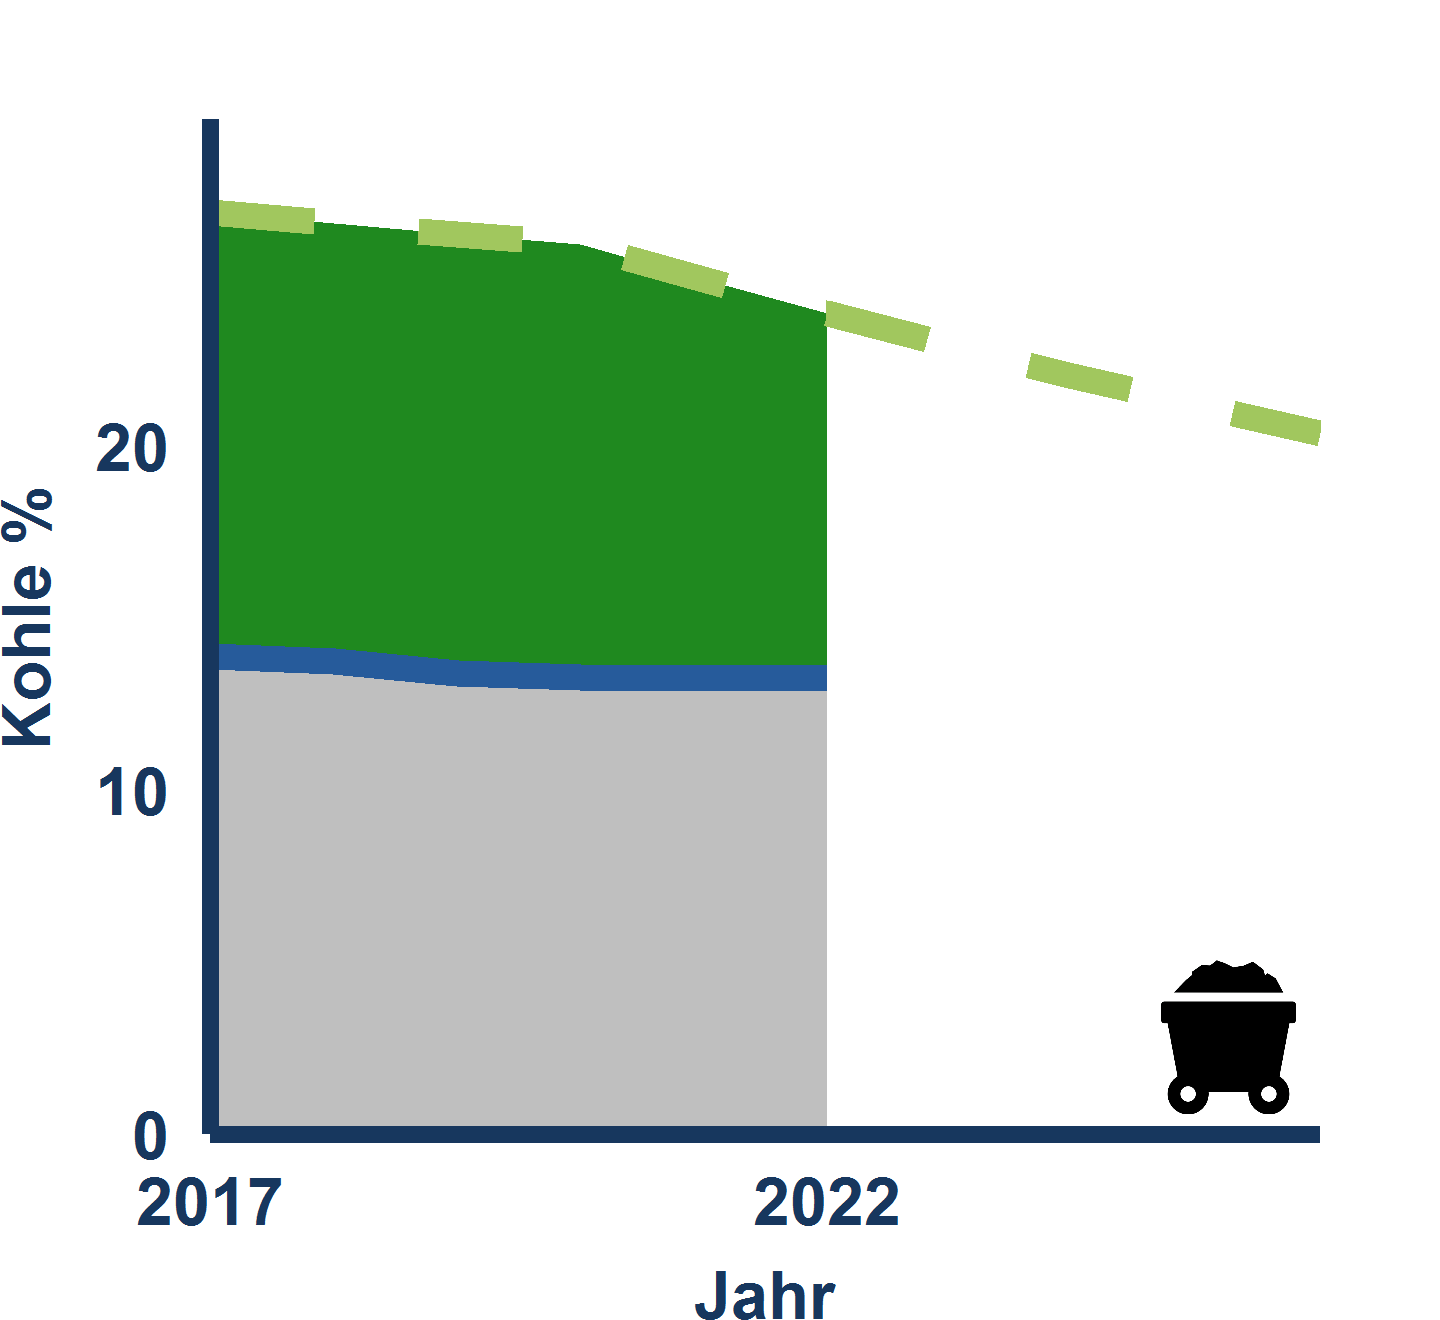
\includegraphics[trim = {0 0cm 0 0},width=1\linewidth]{SwissFigures/Fig10}
			\textbf{CaptionWeight TechCoalCap CBCaptionCoalCap} %CoalCapCBCaption
		\end{minipage}	
		
	{\centering\includegraphics[trim={0 .3cm 0 0.3cm},clip,width=.6\linewidth]{ReportGraphics/LineChartLegend_Languagechoose}\par}

}}

ContentTech2

\fbox{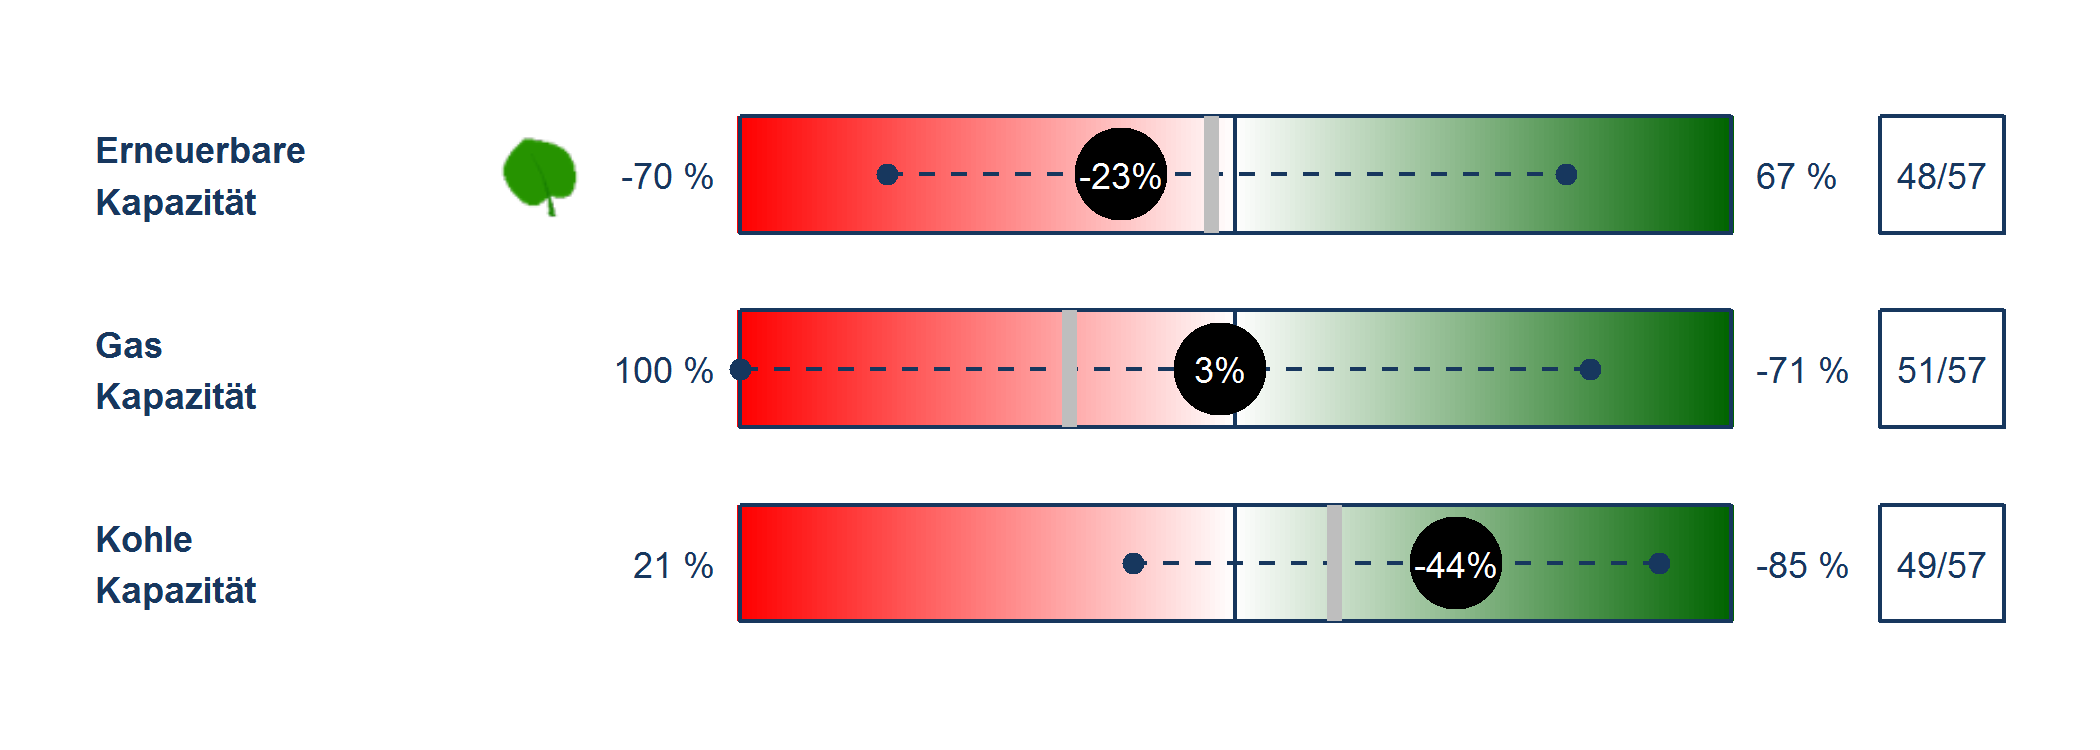
\includegraphics[trim={0 0.9cm 0 0.8cm},clip,width=1\linewidth]{SwissFigures/Fig12}}

\textit{\small SourcePowerFF}

\newpage % PowerCBE  CBPageE
\section*{P12} 		% FossilFuelsEQS EQPageS
\PageHeading{HeadingP12}

ContentP12

\fcolorbox{black}{white}{ 	
	\parbox{1\linewidth}{
		ContentTech1
		
		\vspace{0cm}
		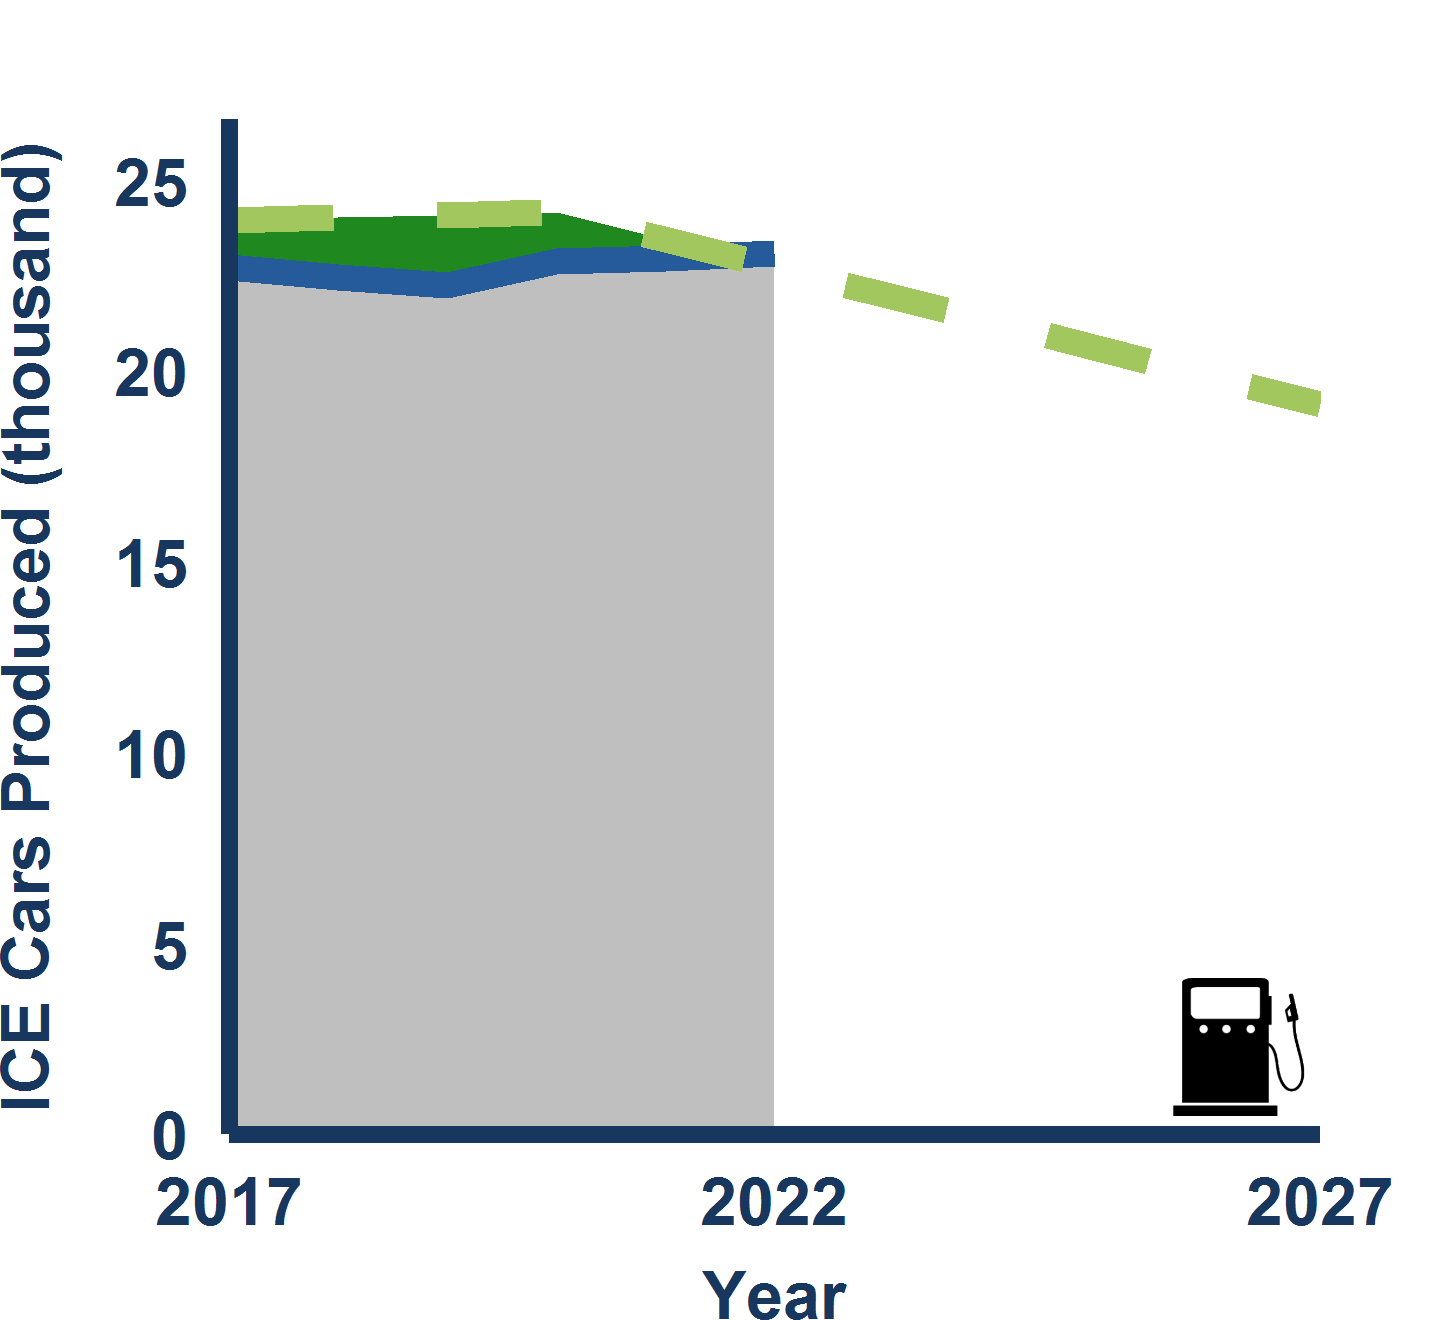
\includegraphics[trim={0 .7cm 0 0},clip,width=1\linewidth]{SwissFigures/Fig23}
		\vspace{-0.5cm}
		\newline
		\begin{minipage}[t]{.32\linewidth}
			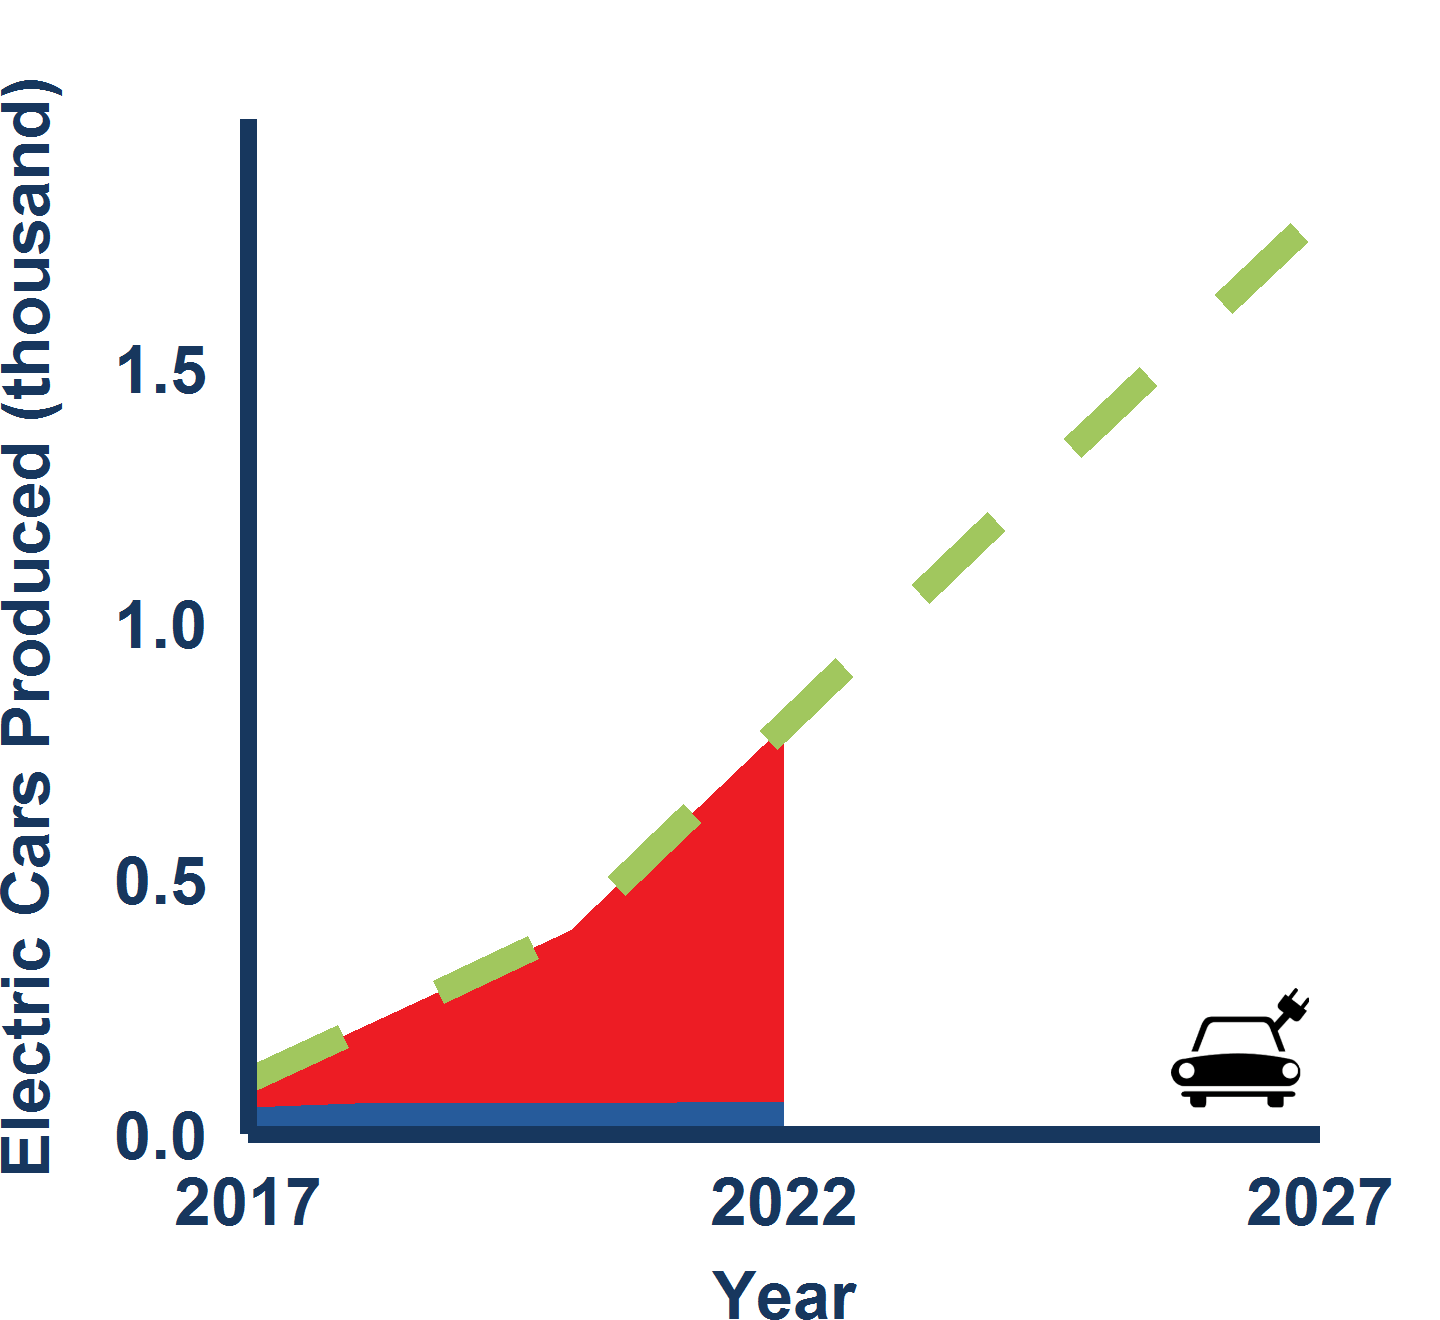
\includegraphics[trim = {0 0cm 0 0},width=1\linewidth]{SwissFigures/Fig24}
			\textbf{CaptionWeight TechOilProd EQCaptionOilProd}
		\end{minipage}	
		\hspace{.01\linewidth}
		\begin{minipage}[t]{.32\textwidth}
			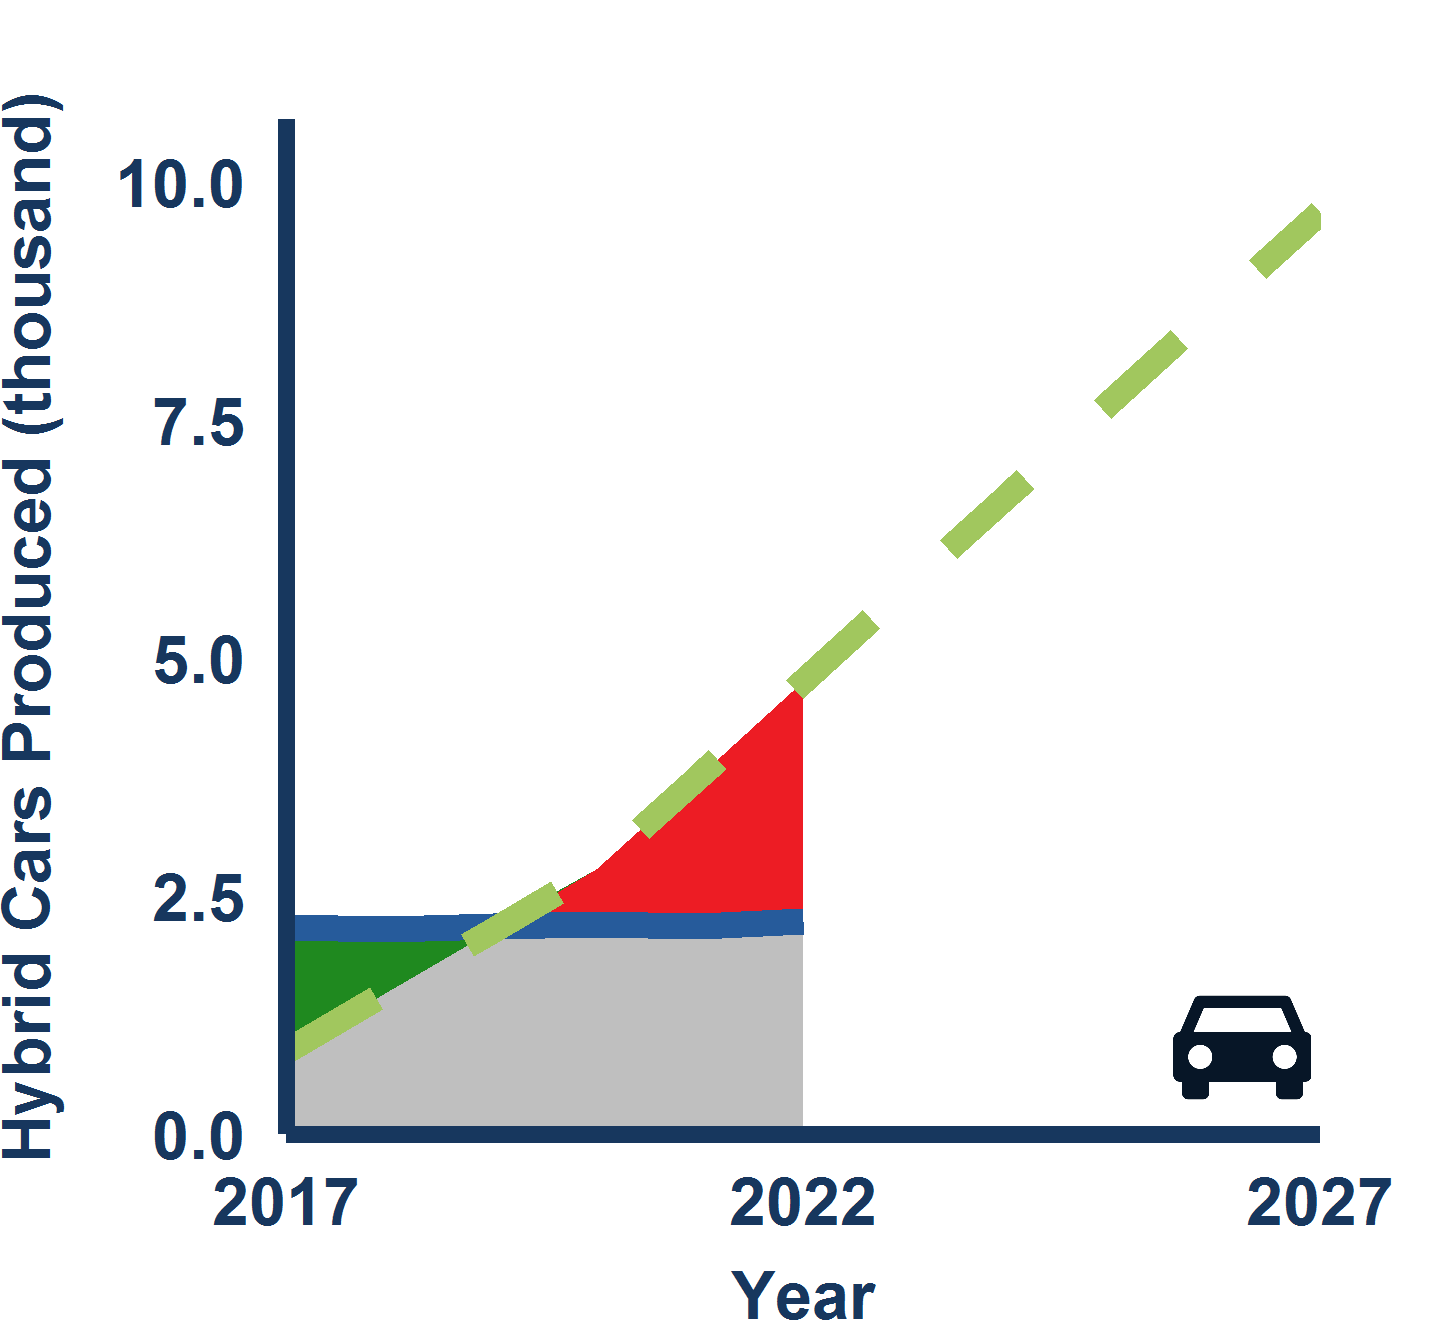
\includegraphics[trim = {0 0cm 0 0},width=1\linewidth]{SwissFigures/Fig25}	
			\textbf{CaptionWeight TechGasProd EQCaptionGasProd}
		\end{minipage}
		\hspace{.01\linewidth}
		\begin{minipage}[t]{.32\linewidth}
			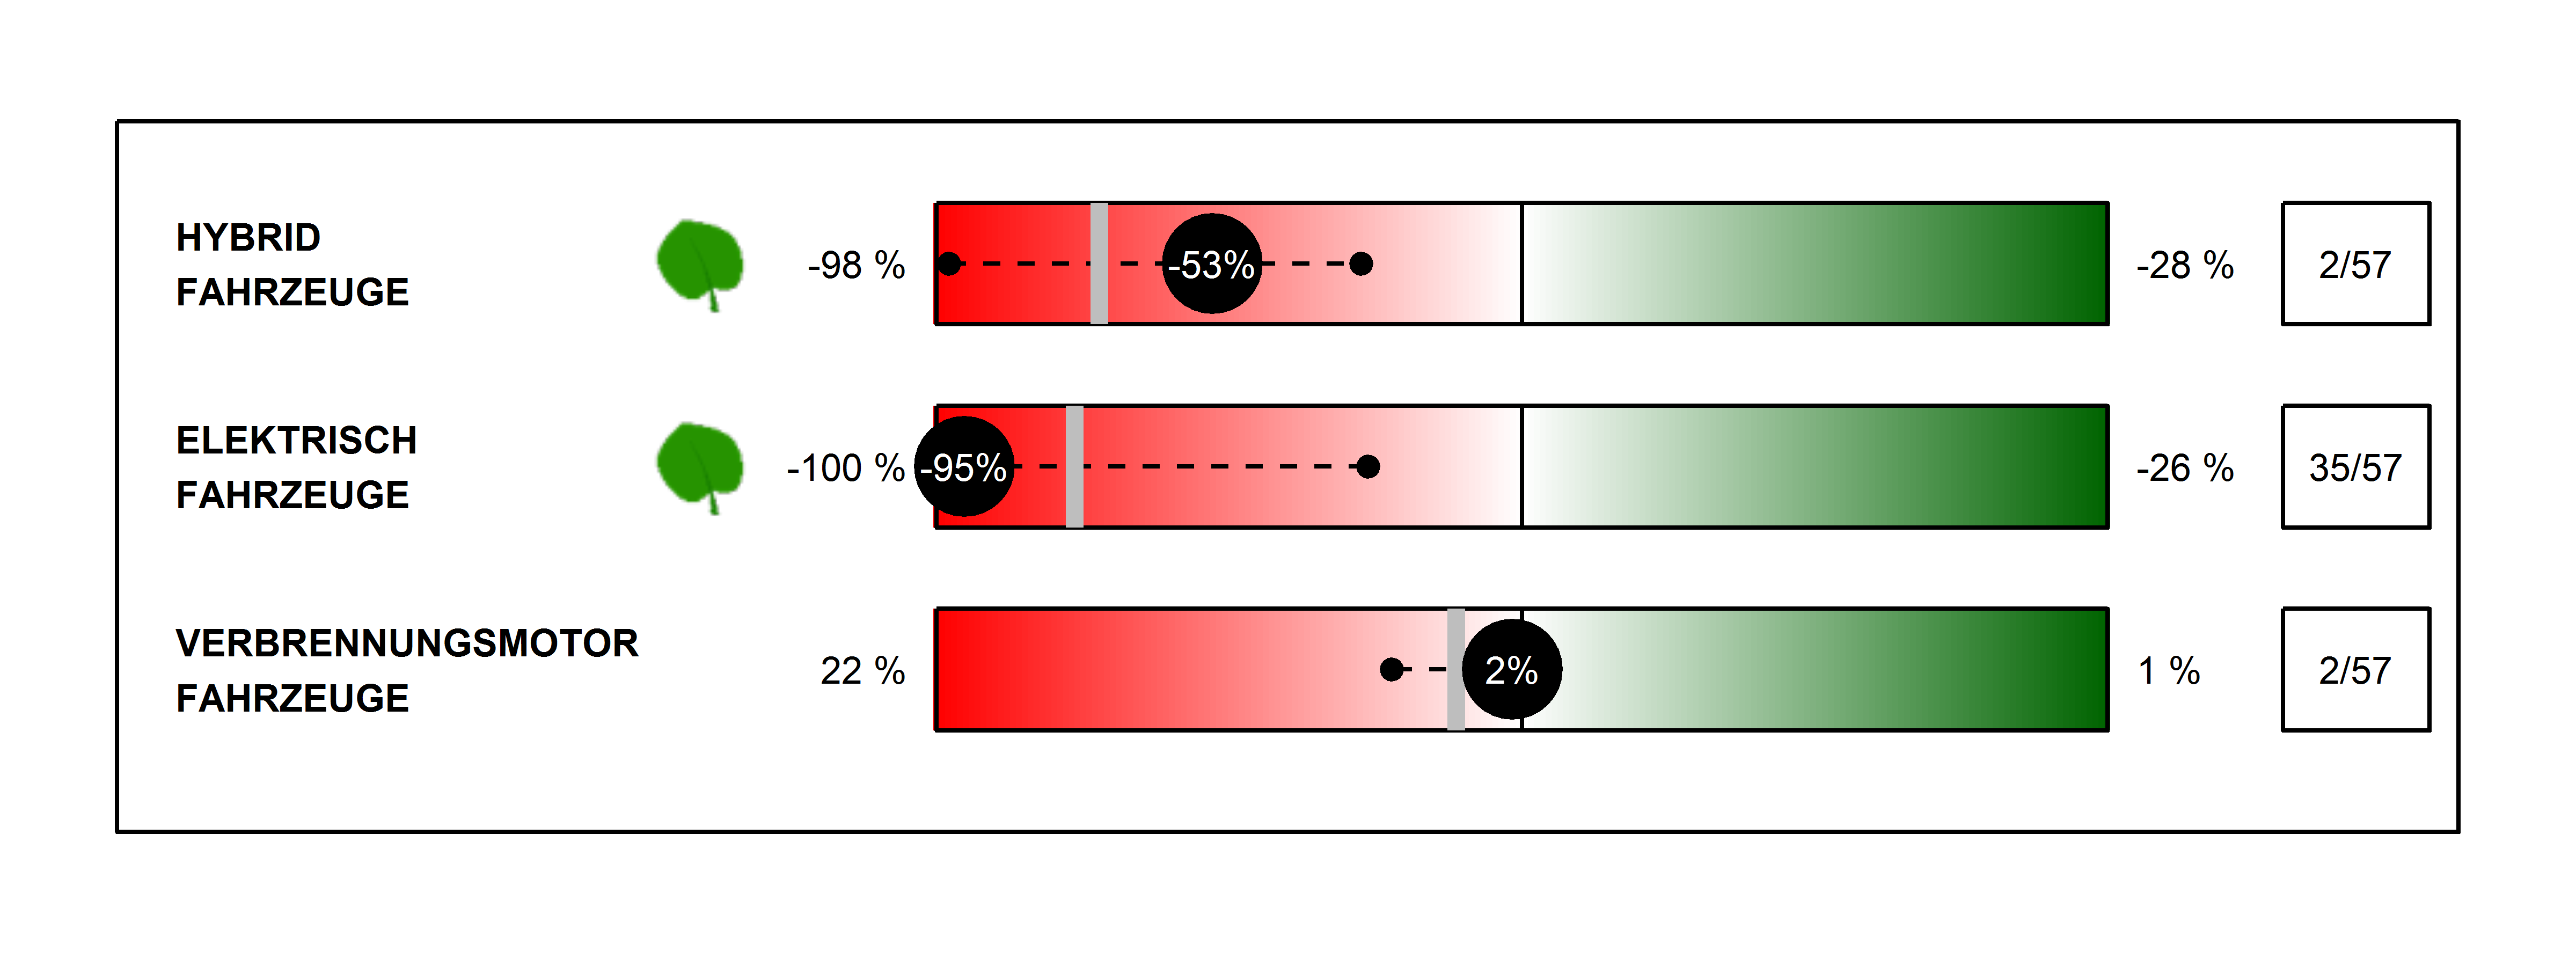
\includegraphics[trim = {0 0cm 0 0},width=1\linewidth]{SwissFigures/Fig26}
			\textbf{CaptionWeight TechCoalProd EQCaptionCoalProd}
		\end{minipage}
			
		{\centering\includegraphics[trim={0 .3cm 0 0.3cm},clip,width=.6\linewidth]{ReportGraphics/LineChartLegend_Languagechoose}\par}
		
}}

ContentTech2

\fbox{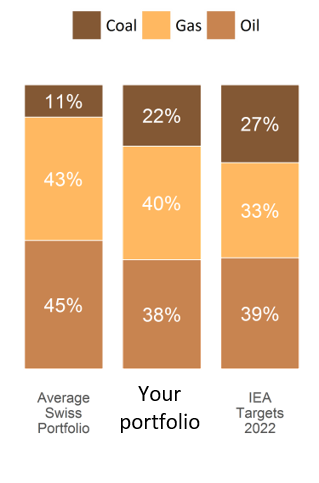
\includegraphics[trim={0 0.9cm 0 0.8cm},clip,width=1\linewidth]{SwissFigures/Fig27}}

\textit{\small SourcePowerFF}

\newpage % FossilFuelsEQE EQPageE
\section*{P13} 		% FossilFuelsCBS  CBPageS
\PageHeading{HeadingP13}

ContentP13

\fcolorbox{black}{white}{ 	
	\parbox{1\linewidth}{
		ContentTech1
		
		\vspace{0cm}
		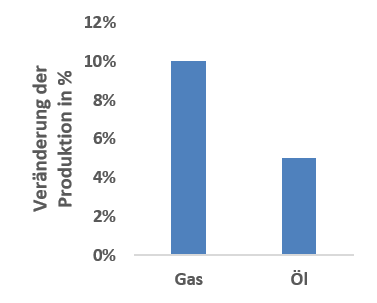
\includegraphics[trim={0 .7cm 0 0},clip,width=1\linewidth]{SwissFigures/Fig28}
		\vspace{-0.5cm}
		\newline
		\begin{minipage}[t]{.32\linewidth}
			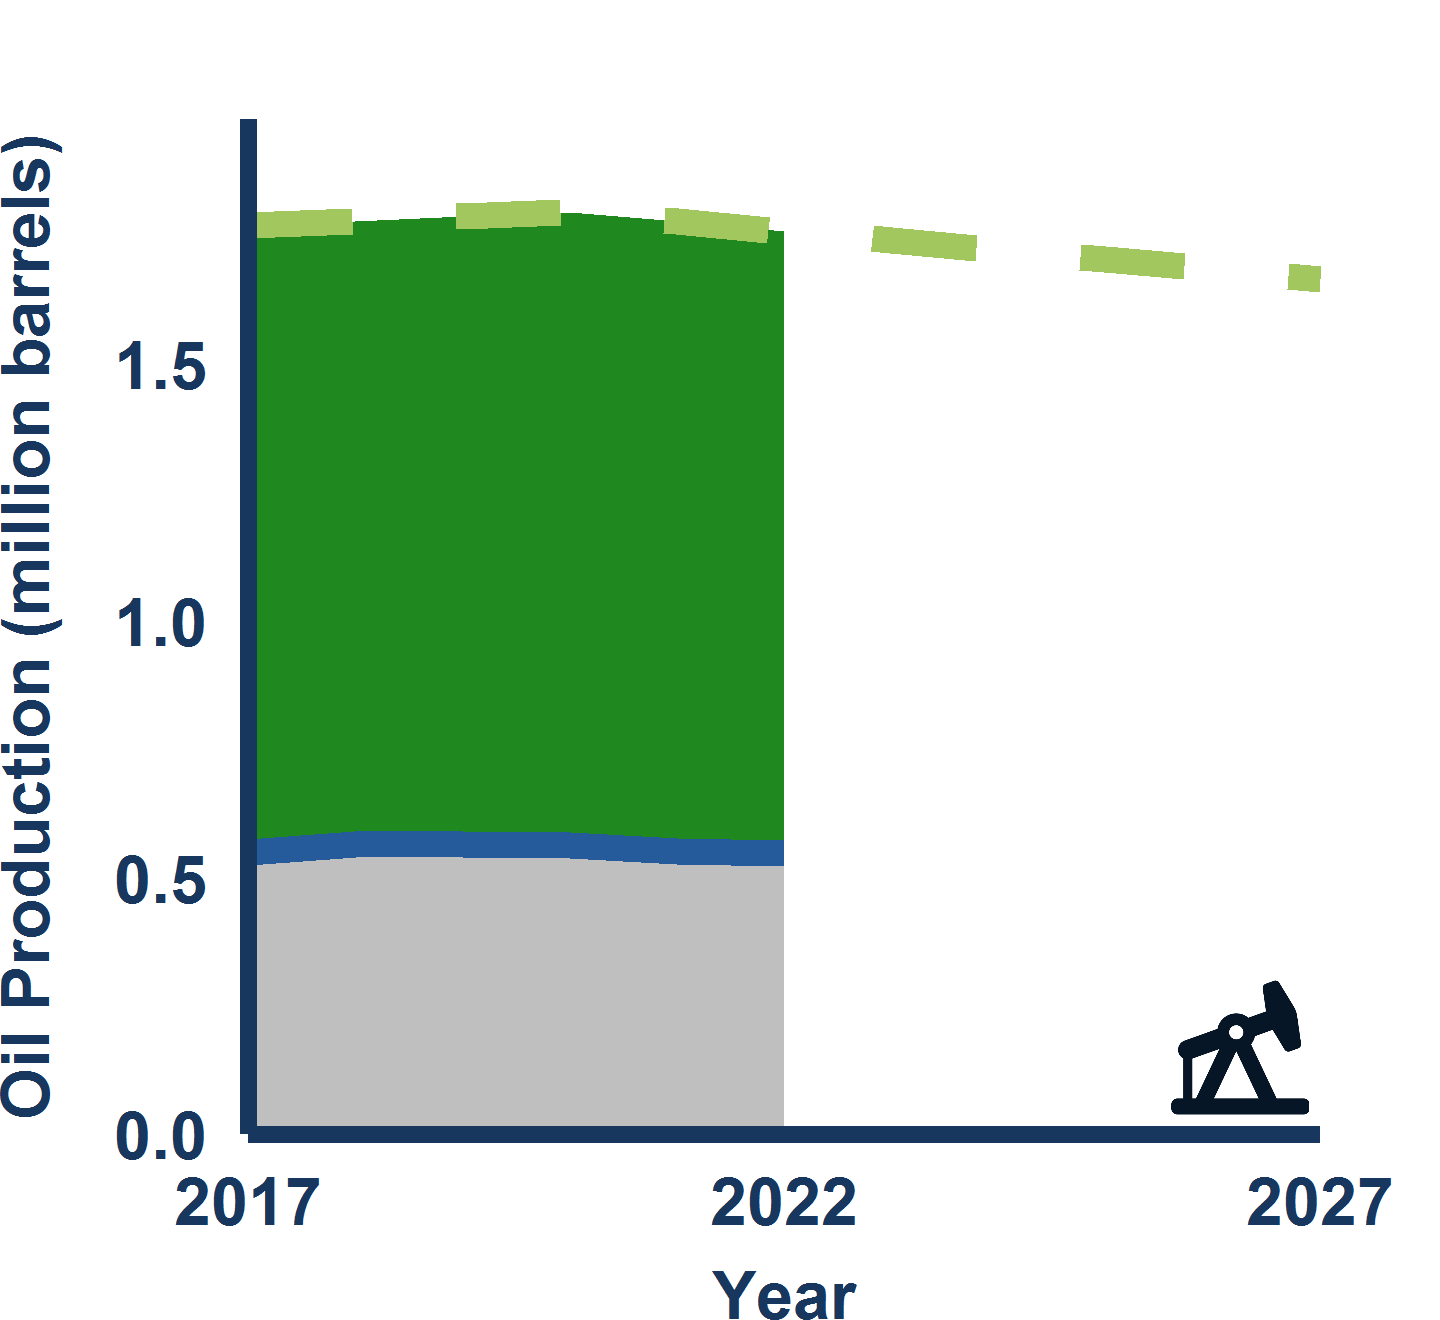
\includegraphics[trim = {0 0cm 0 0},width=1\linewidth]{SwissFigures/Fig29}
			\textbf{CaptionWeight TechOilProd CBCaptionOilProd}
		\end{minipage}	
		\hspace{.01\linewidth}
		\begin{minipage}[t]{.32\textwidth}
			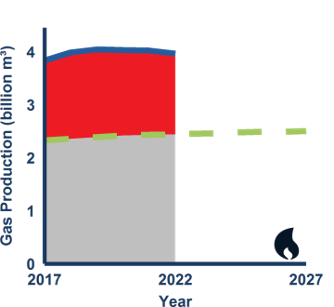
\includegraphics[trim = {0 0cm 0 0},width=1\linewidth]{SwissFigures/Fig30}	
			\textbf{CaptionWeight TechGasProd CBCaptionGasProd}
		\end{minipage}
		\hspace{.01\linewidth}
		\begin{minipage}[t]{.32\linewidth}
			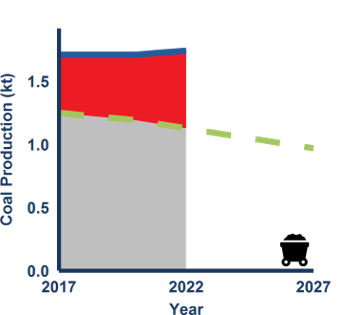
\includegraphics[trim = {0 0cm 0 0},width=1\linewidth]{SwissFigures/Fig31}
			\textbf{CaptionWeight TechCoalProd CBCaptionCoalProd}
		\end{minipage}	
		
		{\centering\includegraphics[trim={0 .3cm 0 0.3cm},clip,width=.6\linewidth]{ReportGraphics/LineChartLegend_Languagechoose}\par}
		
}}

ContentTech2

\fbox{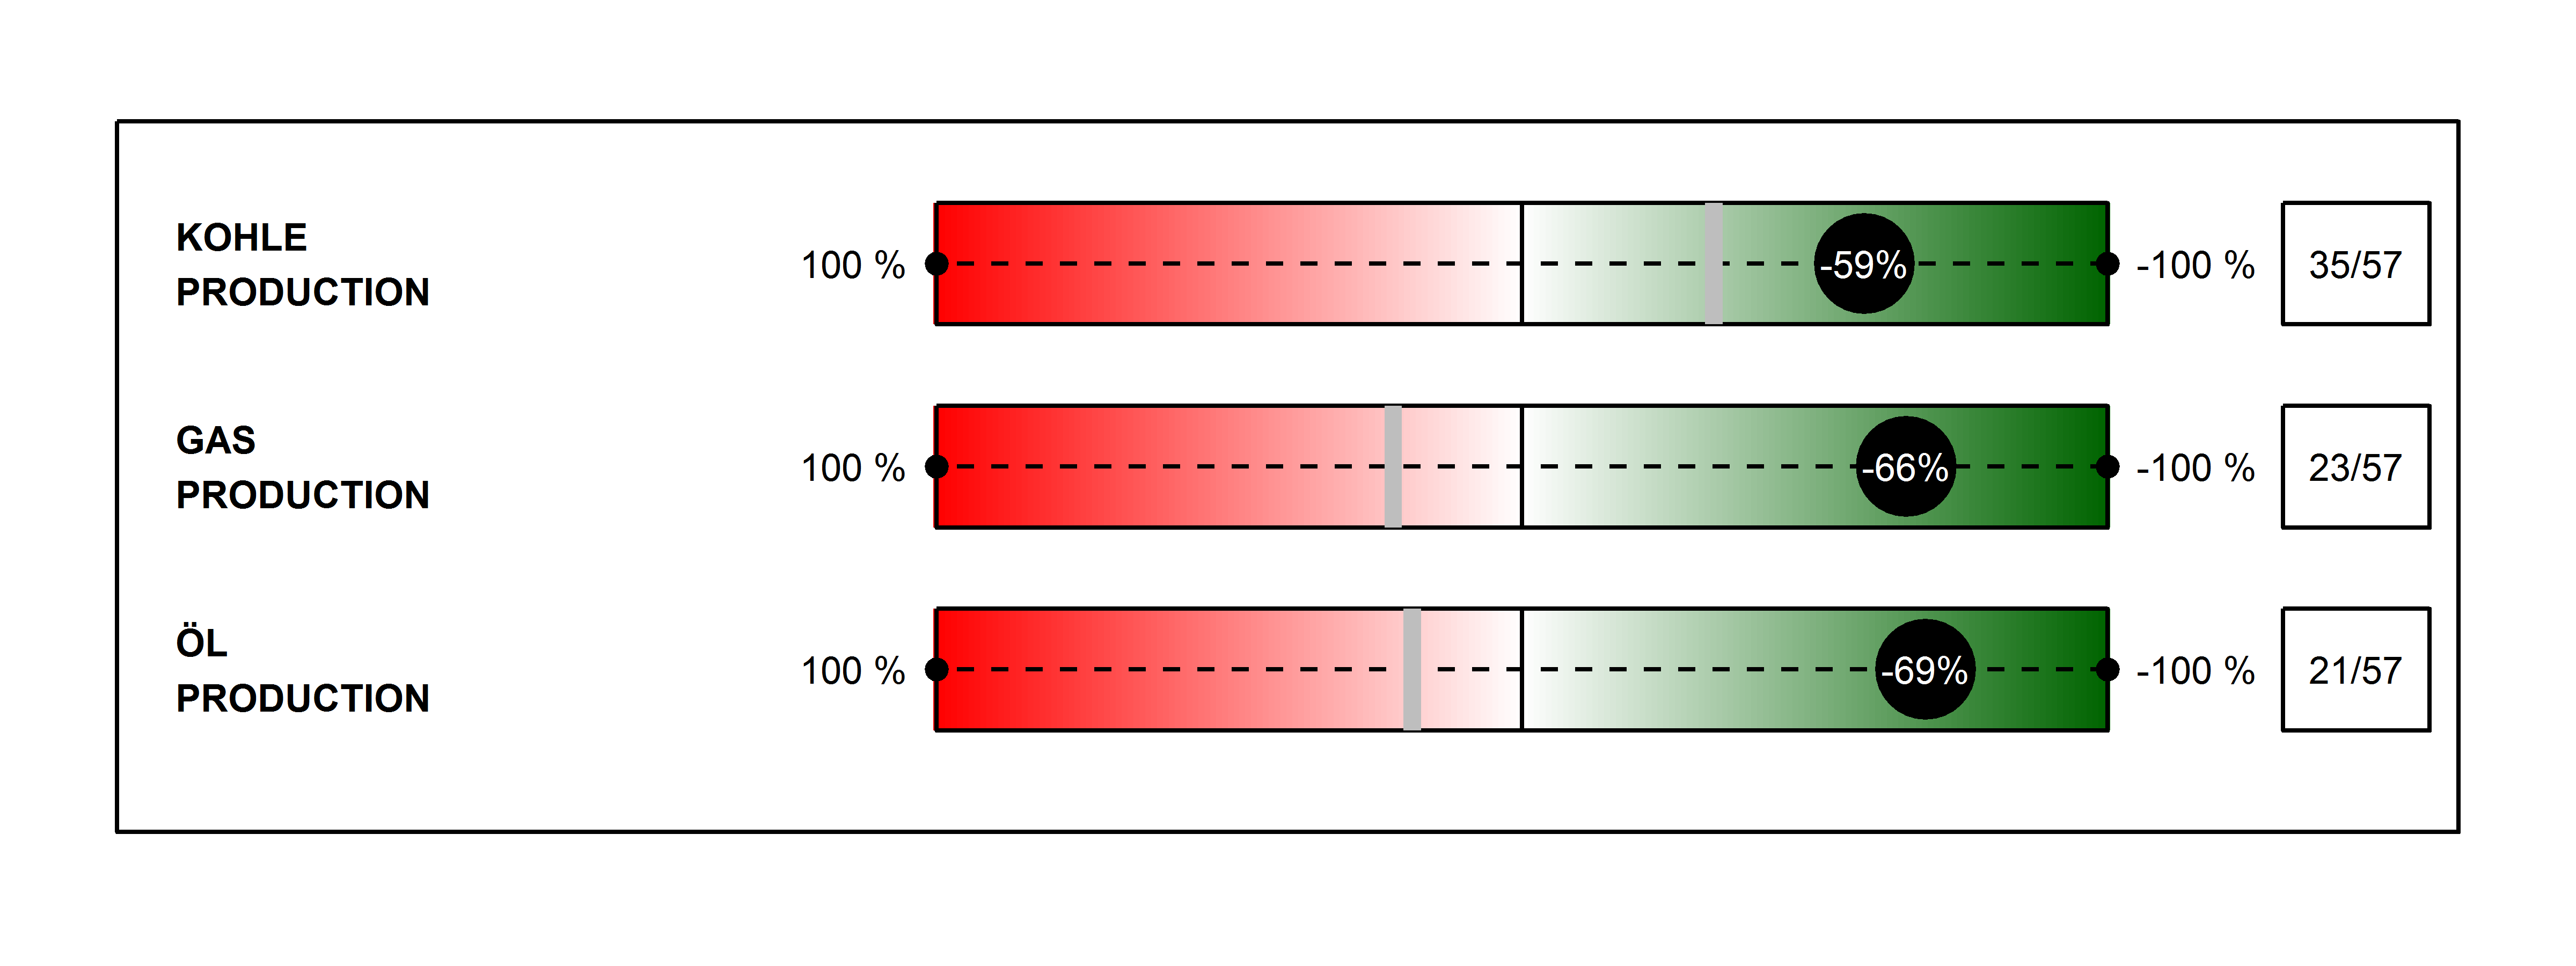
\includegraphics[trim={0 0.9cm 0 0.8cm},clip,width=1\linewidth]{SwissFigures/Fig32}}

\textit{\small SourcePowerFF}
\newpage % FossilFuelsCBE  CBPageE
\section*{P10} 		% AutomotiveEQS EQPageS
\PageHeading{HeadingP10}

ContentP10

\fcolorbox{black}{white}{ 	
	\parbox{1\linewidth}{
		ContentTech1
		
		\vspace{0cm}
		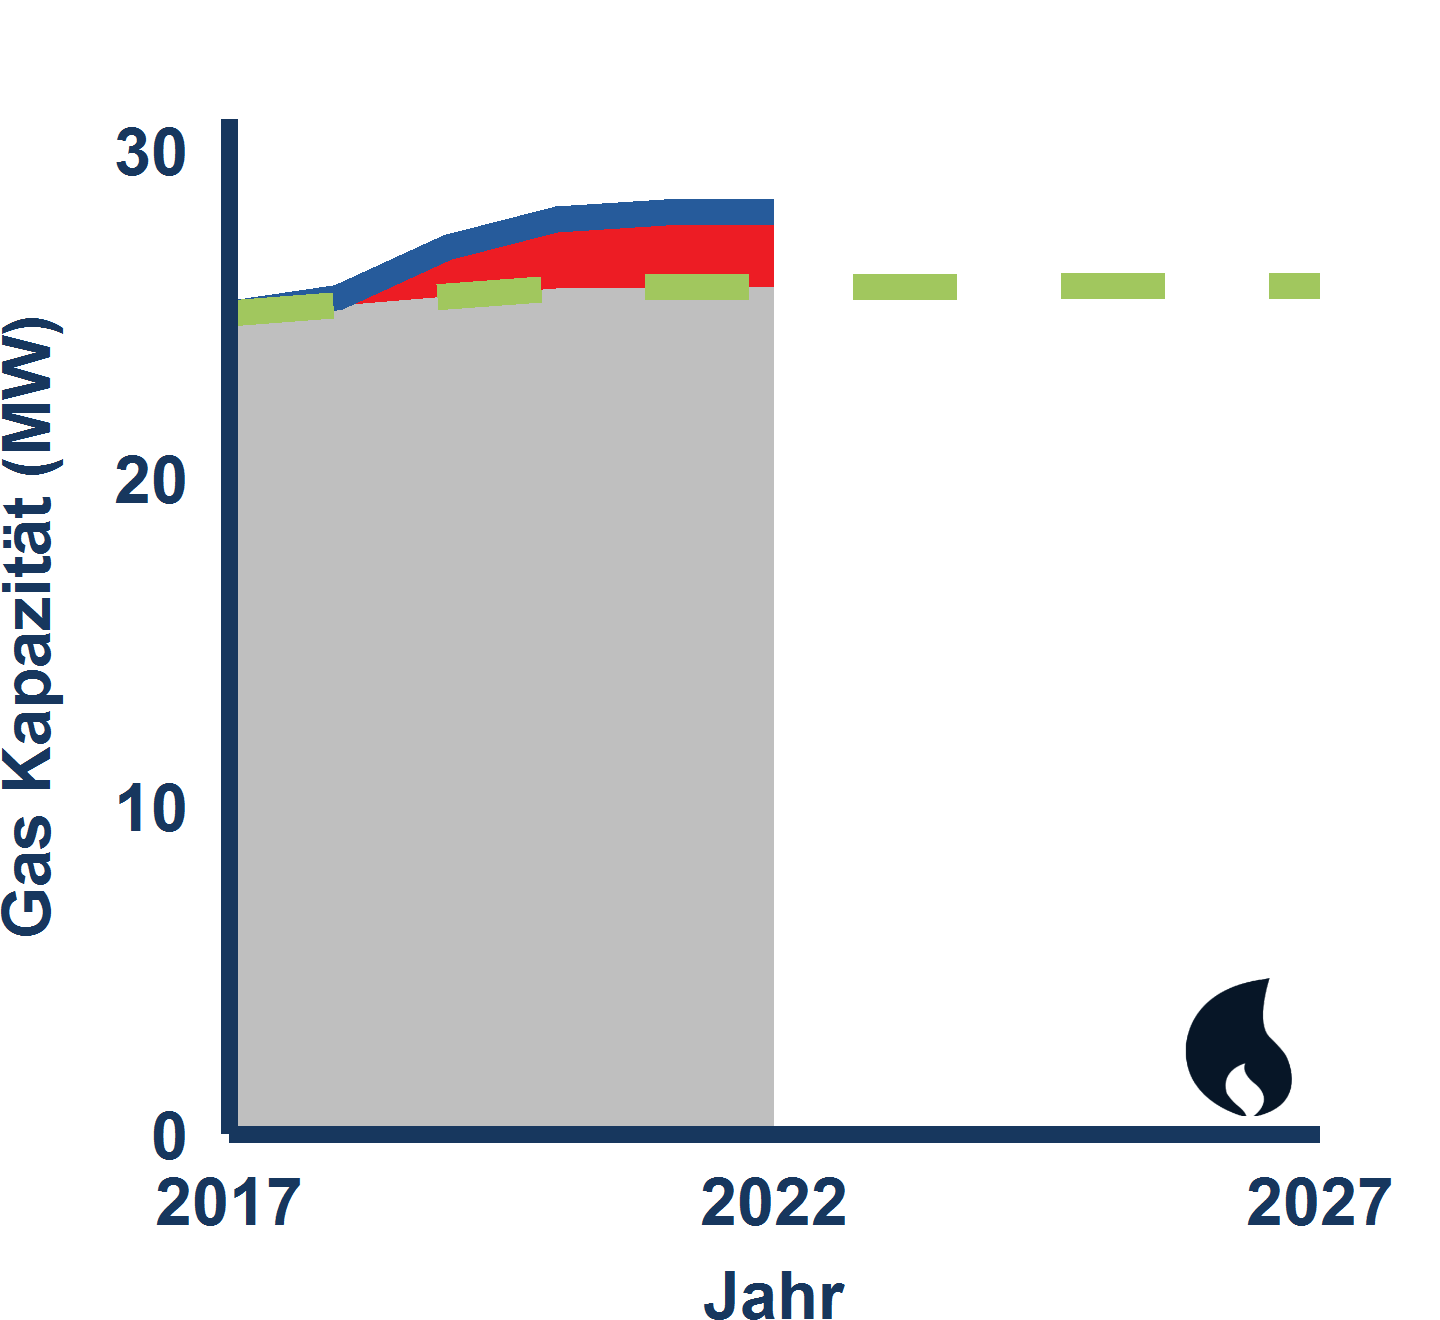
\includegraphics[trim={0 .7cm 0 0},clip,width=1\linewidth]{SwissFigures/Fig13}
		\vspace{-0.5cm}
		\newline
		\begin{minipage}[t]{.32\linewidth}
			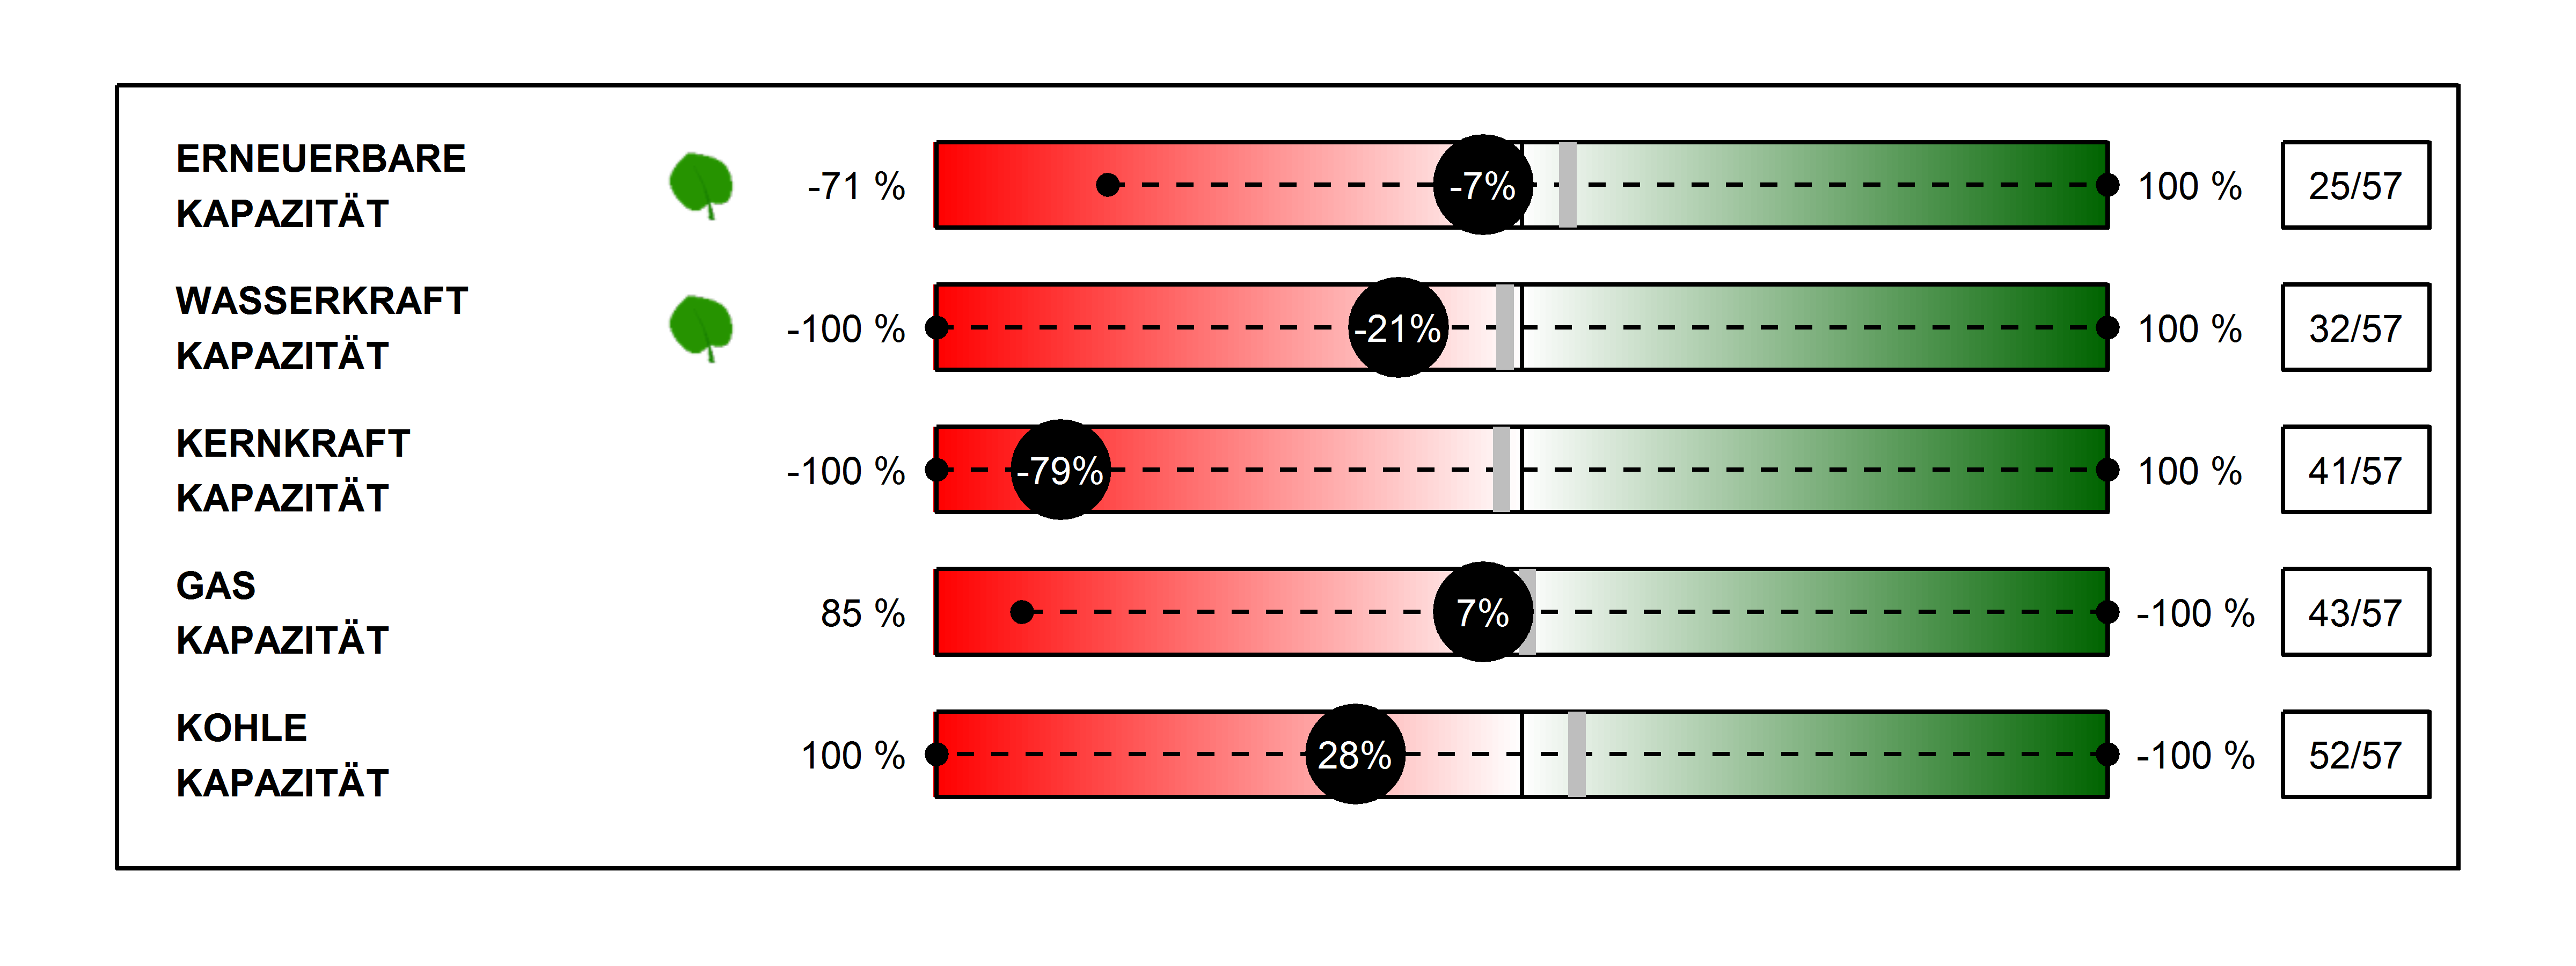
\includegraphics[trim = {0 0cm 0 0},width=1\linewidth]{SwissFigures/Fig14}
			\textbf{CaptionWeight TechICE EQCaptionICE}
		\end{minipage}	
		\hspace{.01\linewidth}
		\begin{minipage}[t]{.32\textwidth}
			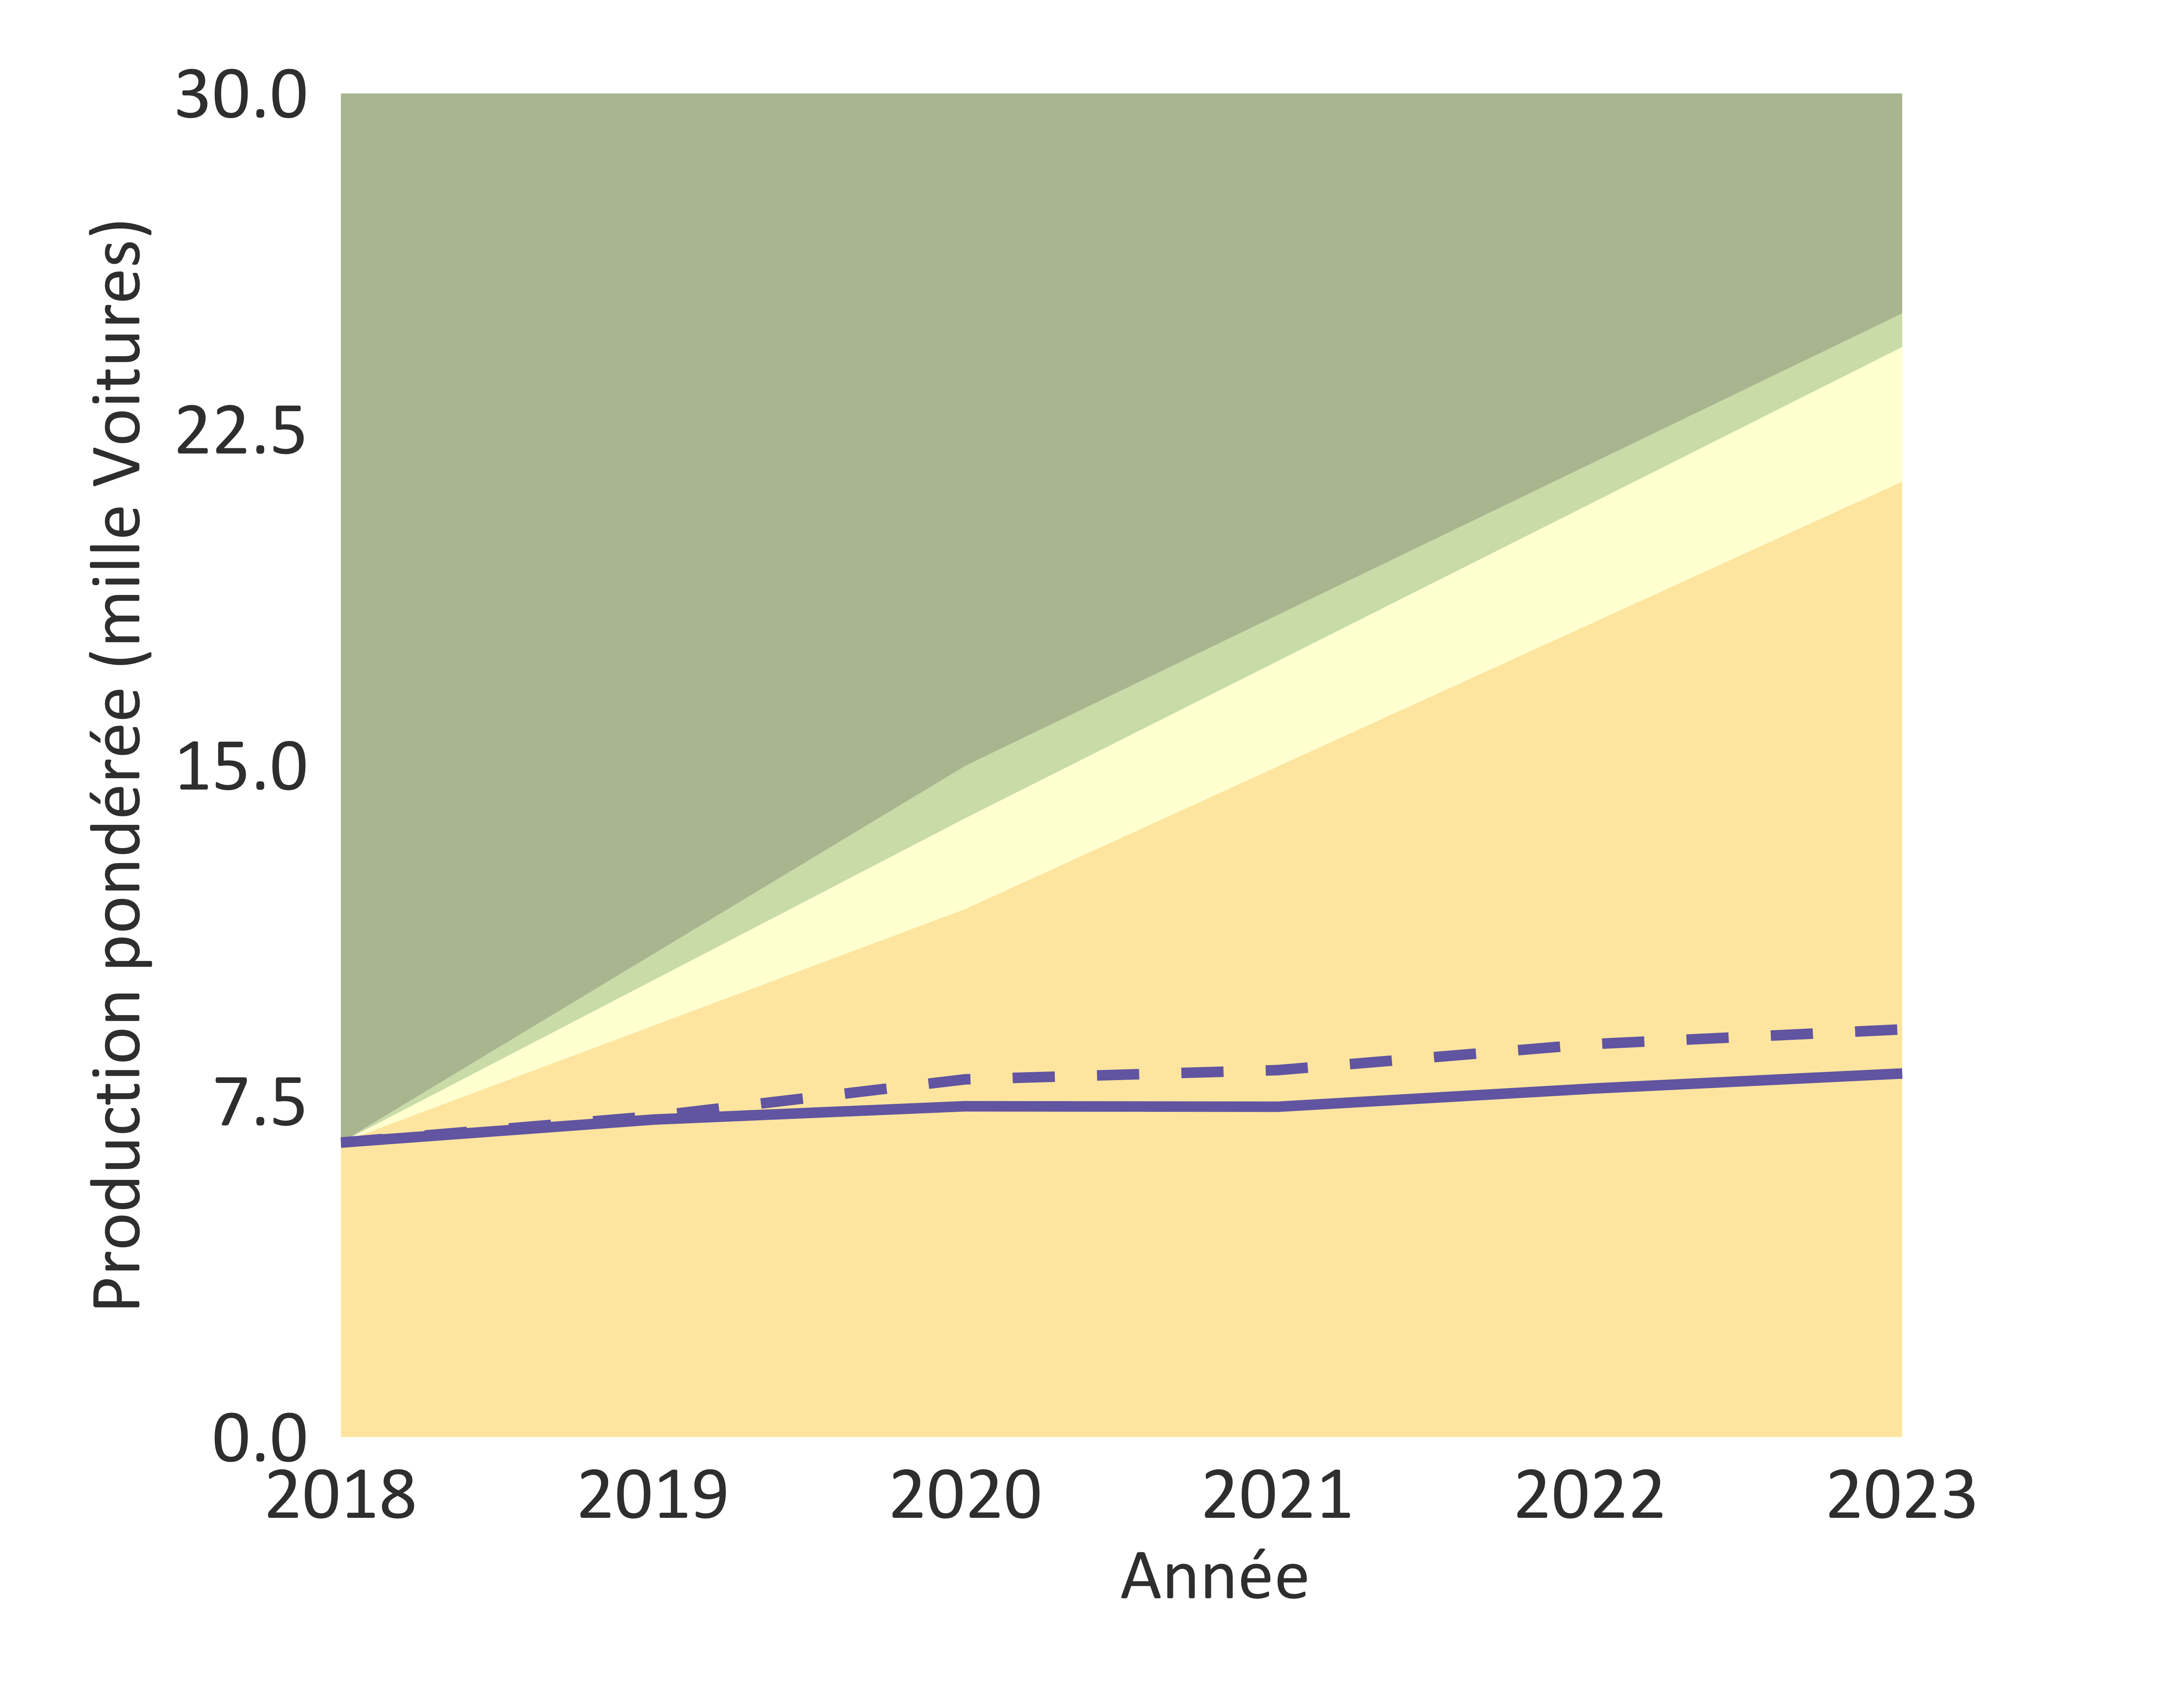
\includegraphics[trim = {0 0cm 0 0},width=1\linewidth]{SwissFigures/Fig16}	
			\textbf{CaptionWeight TechHybrid EQCaptionHybrid}
			
		\end{minipage}
		\hspace{.01\linewidth}
		\begin{minipage}[t]{.32\linewidth}
			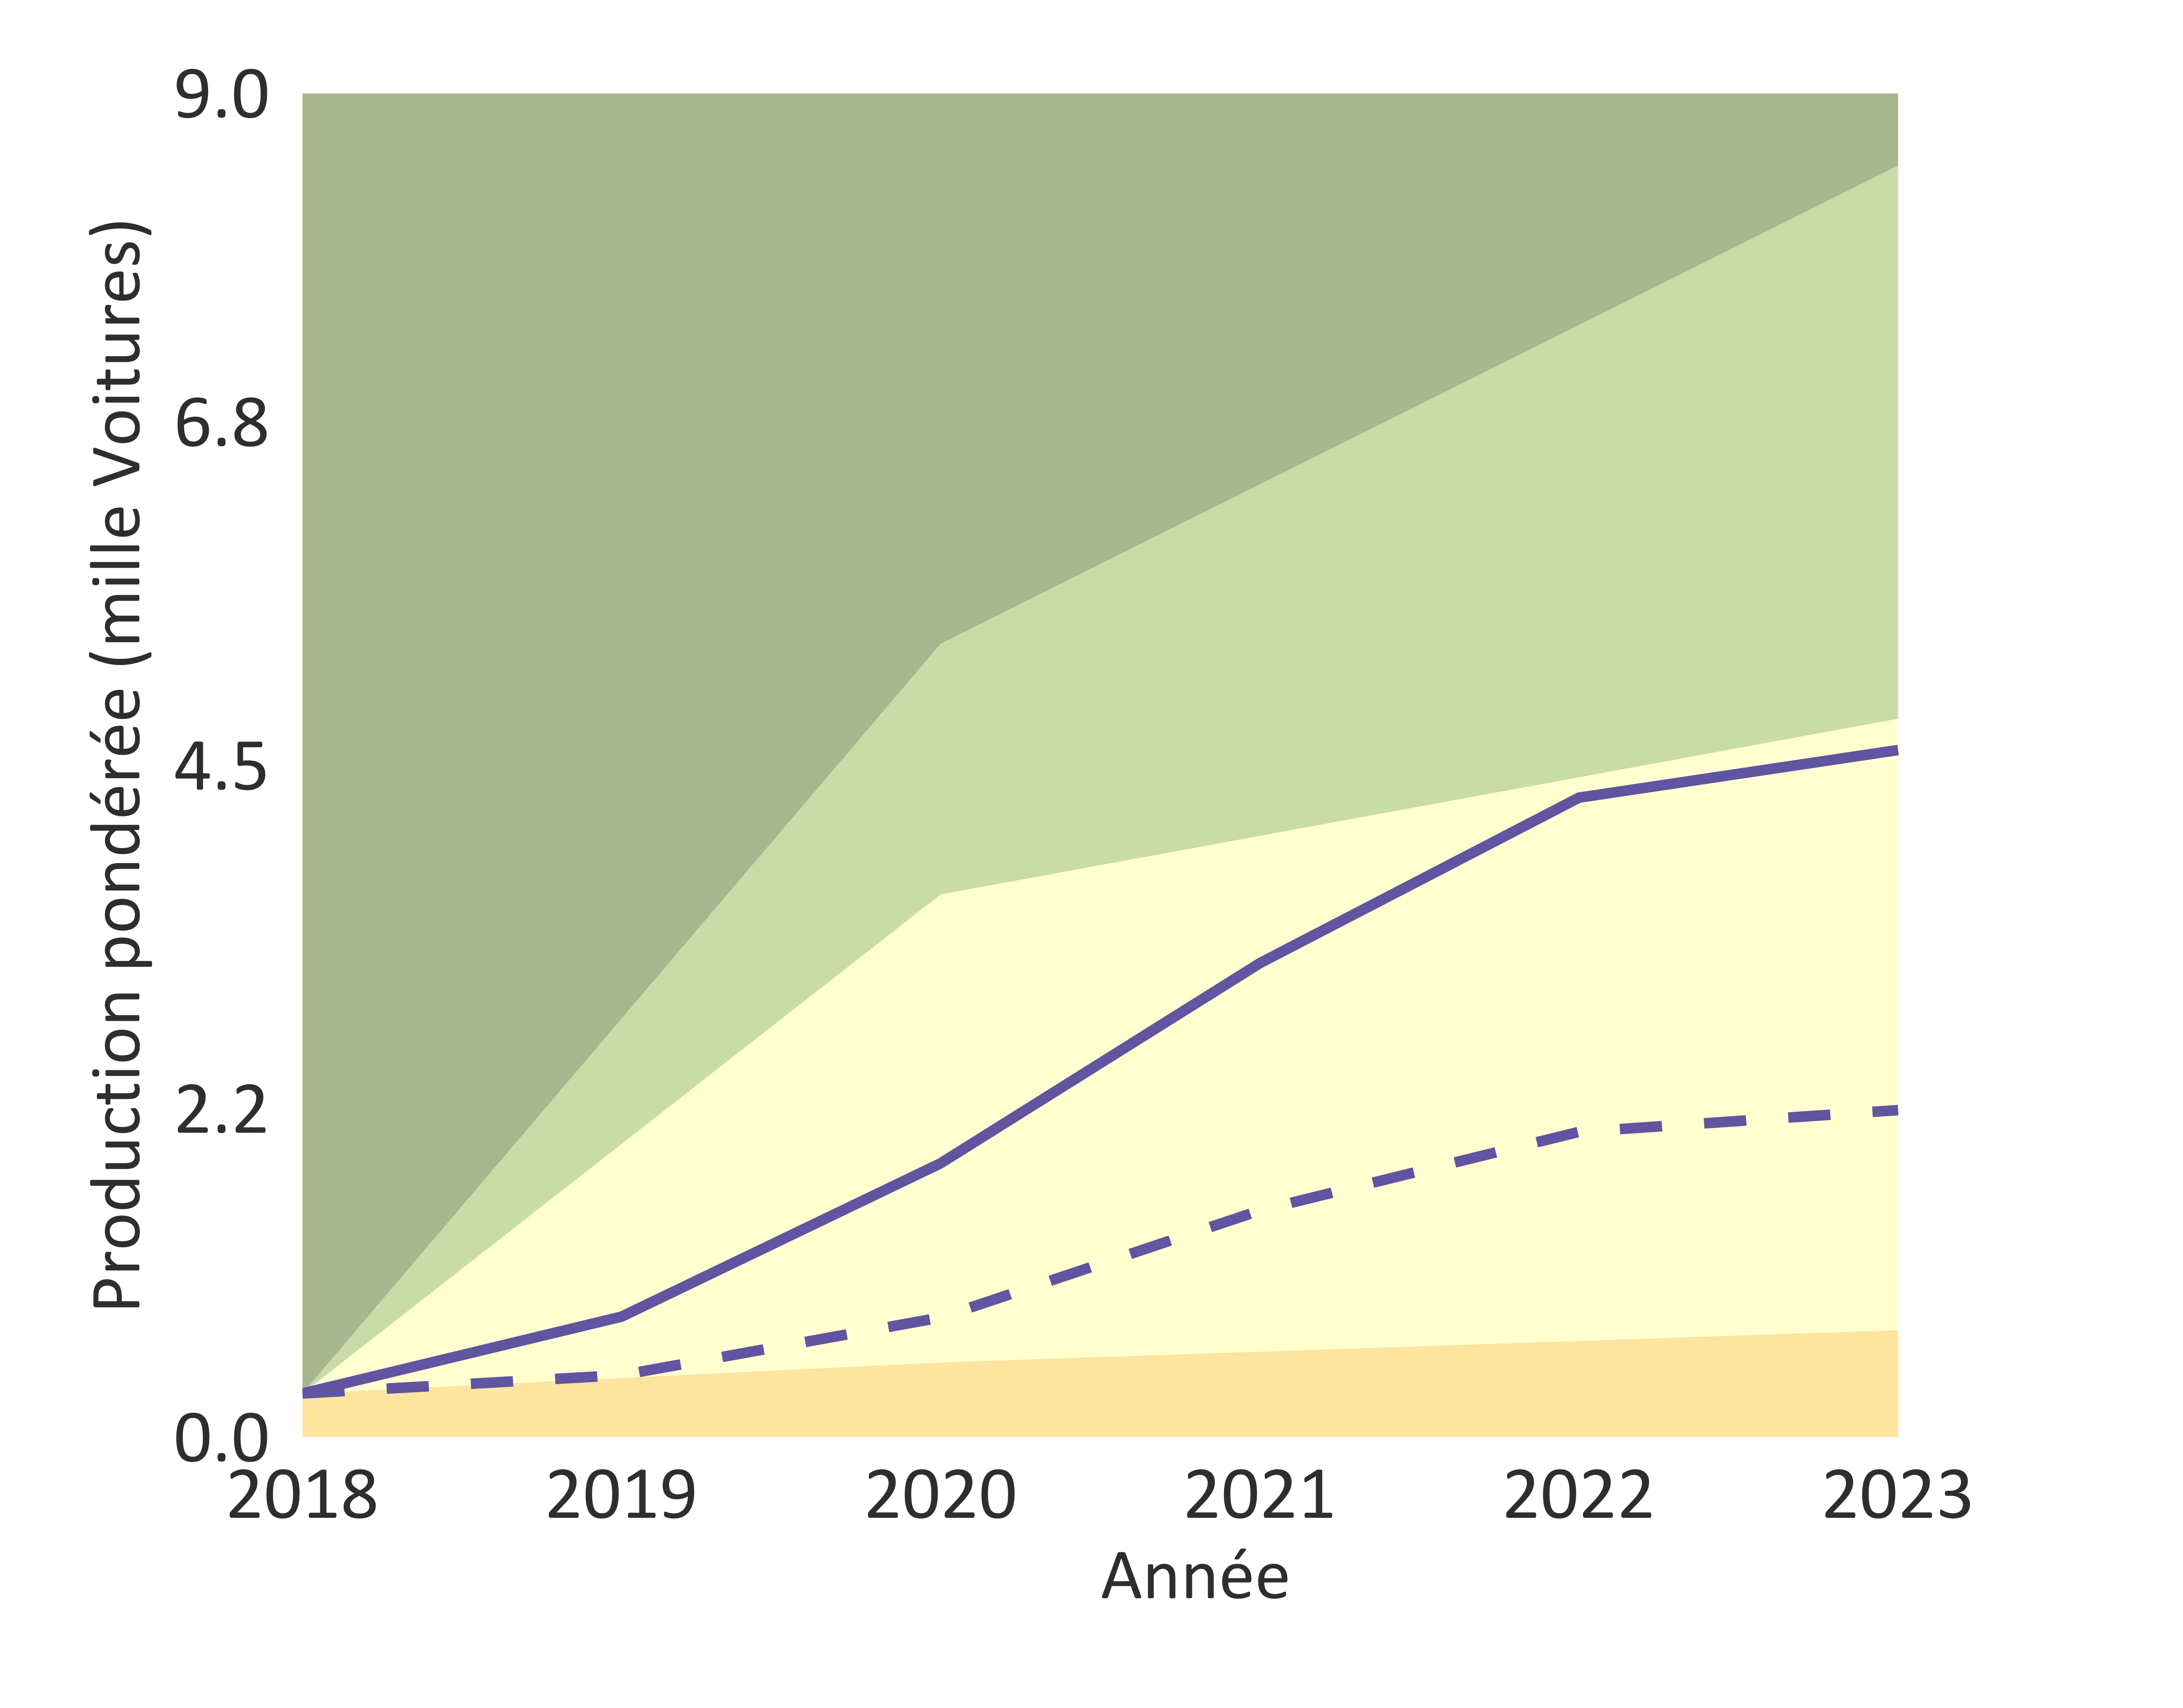
\includegraphics[trim = {0 0cm 0 0},width=1\linewidth]{SwissFigures/Fig15}
			\textbf{CaptionWeight TechElectric EQCaptionElectric}
		\end{minipage}	
		
		{\centering\includegraphics[trim={0 .3cm 0 0.3cm},clip,width=.6\linewidth]{ReportGraphics/LineChartLegend_Languagechoose}\par}
		
}}

ContentTech2

\fbox{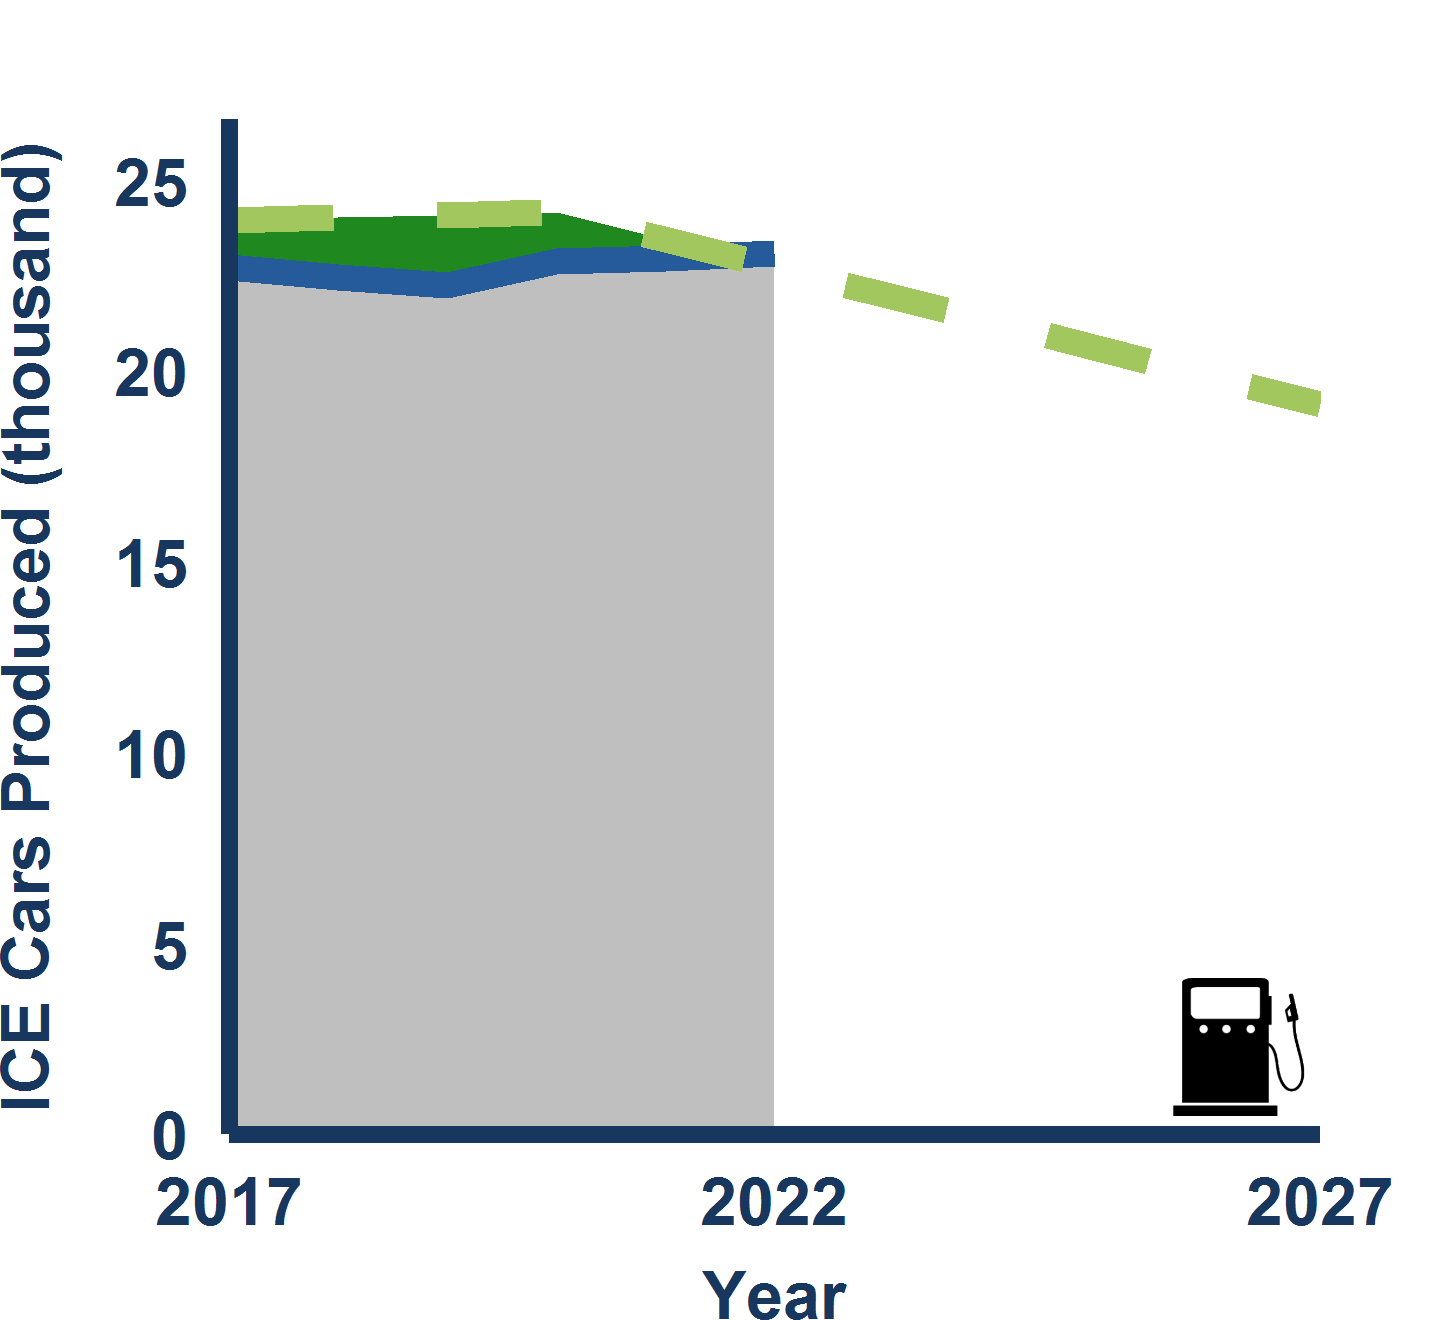
\includegraphics[trim={0 0.9cm 0 0.8cm},clip,width=1\linewidth]{SwissFigures/Fig17}}

\textit{\small SourceAuto}

\newpage %AutomotiveEQE EQPageE
\section*{P11} 		% AutomotiveCBS CBPageS
\PageHeading{HeadingP11}

ContentP11

\fcolorbox{black}{white}{ 	
	\parbox{1\linewidth}{
		ContentTech1
		
		\vspace{0cm}
		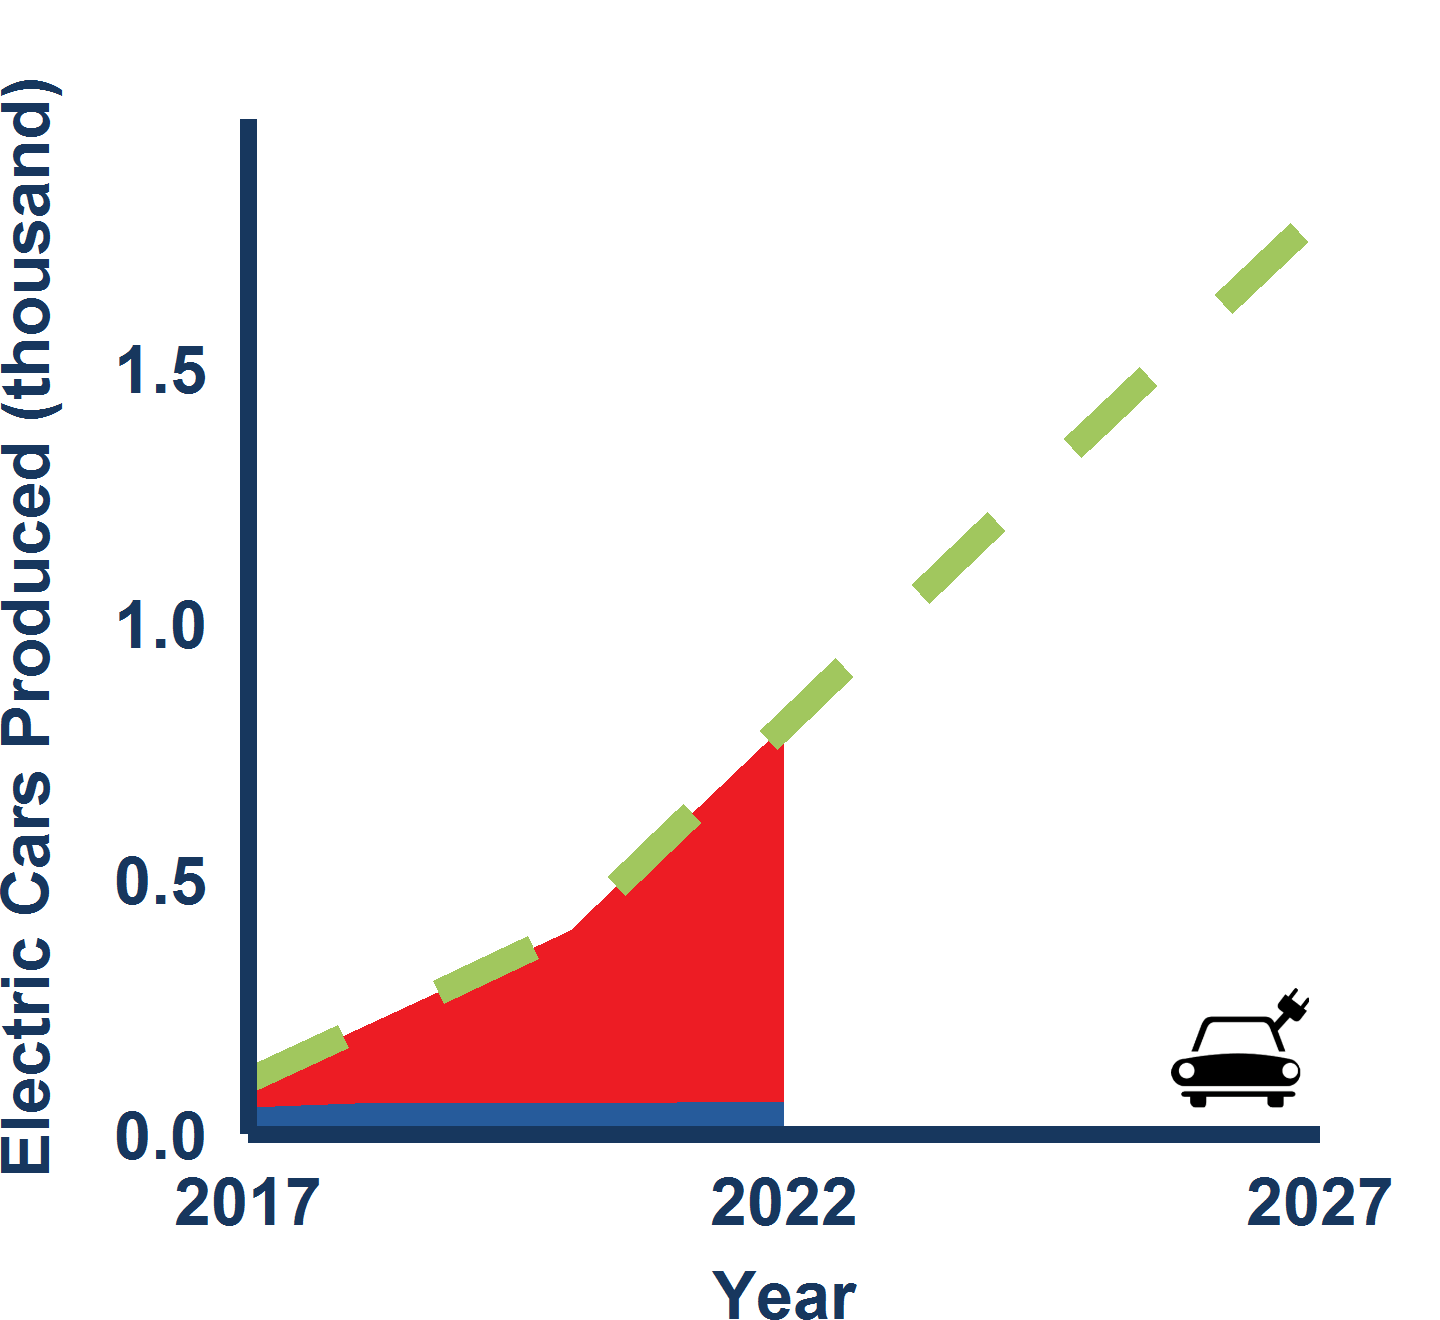
\includegraphics[trim={0 .7cm 0 0},clip,width=1\linewidth]{SwissFigures/Fig18}
		\vspace{-0.5cm}
		\newline
		\begin{minipage}[t]{.32\linewidth}
			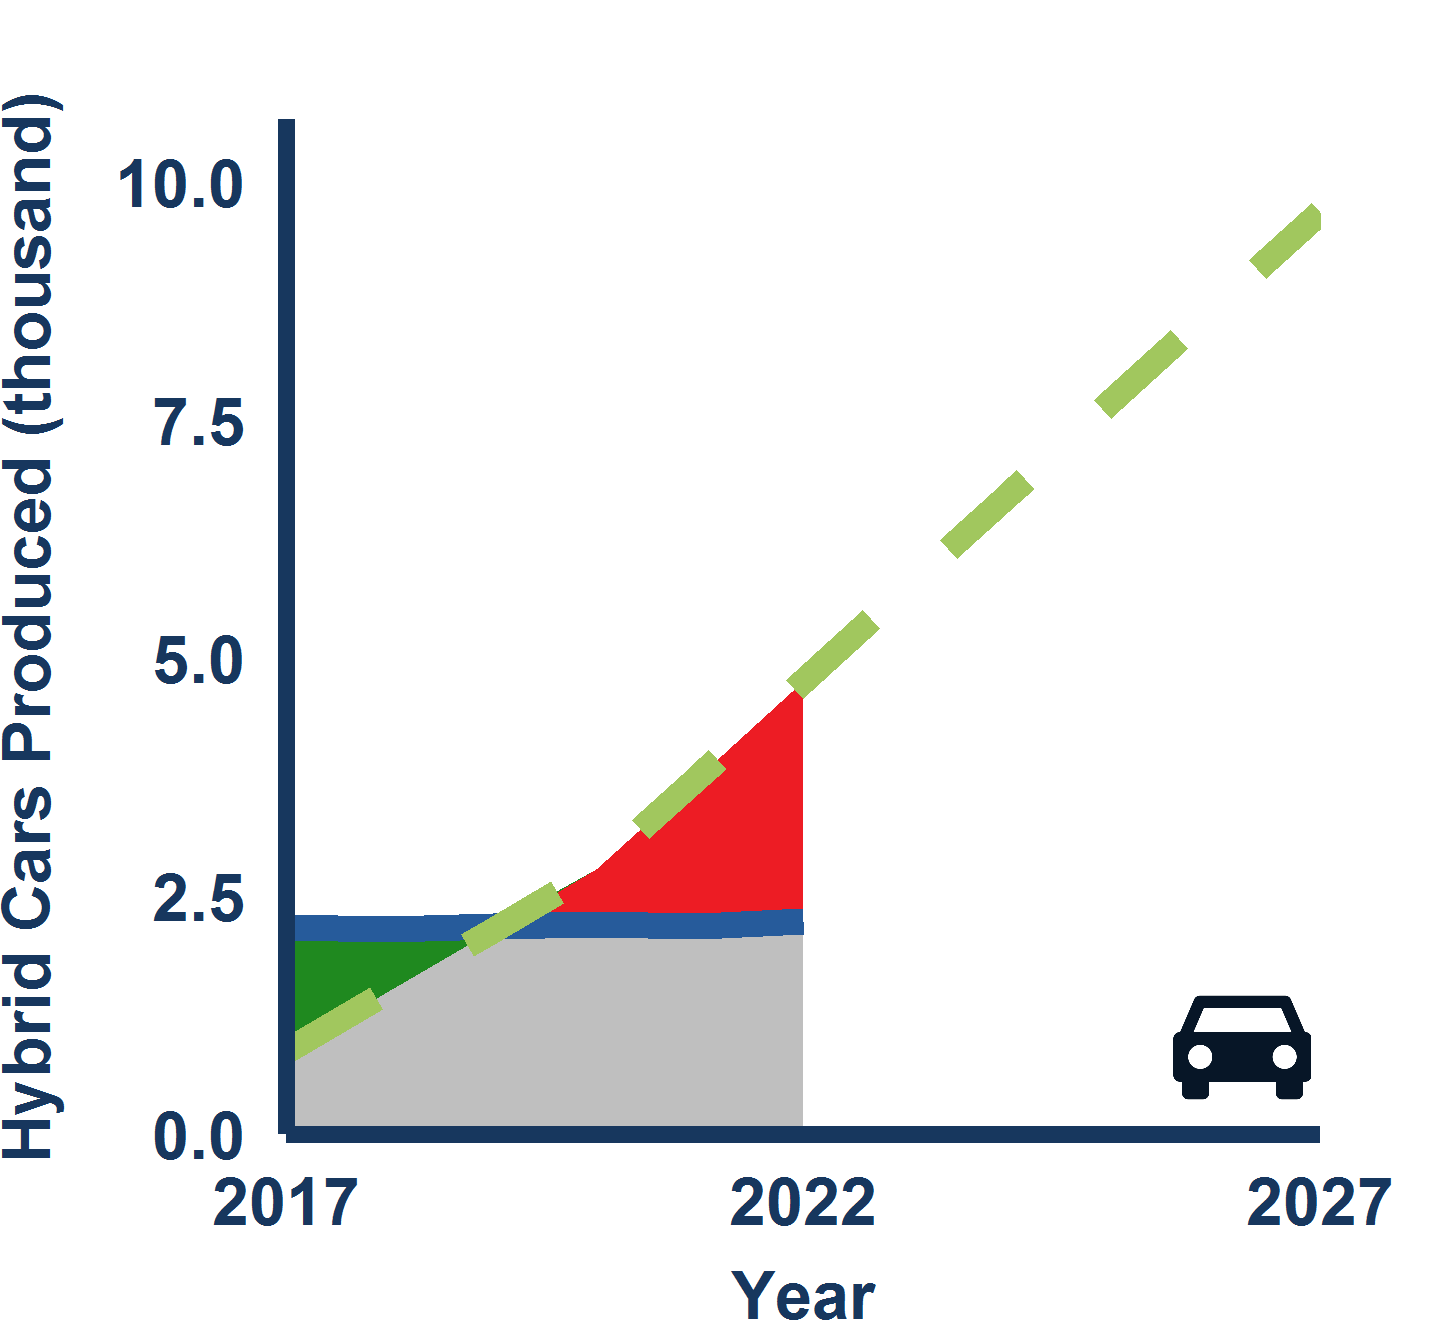
\includegraphics[trim = {0 0cm 0 0},width=1\linewidth]{SwissFigures/Fig19}
			\textbf{CaptionWeight TechICE CBCaptionICE}
		\end{minipage}	
		\hspace{.01\linewidth}
		\begin{minipage}[t]{.32\textwidth}
			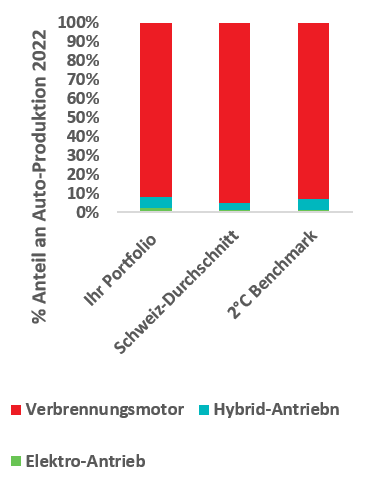
\includegraphics[trim = {0 0cm 0 0},width=1\linewidth]{SwissFigures/Fig21}	
			\textbf{CaptionWeight TechHybrid CBCaptionHybrid}
		\end{minipage}
		\hspace{.01\linewidth}
		\begin{minipage}[t]{.32\linewidth}
			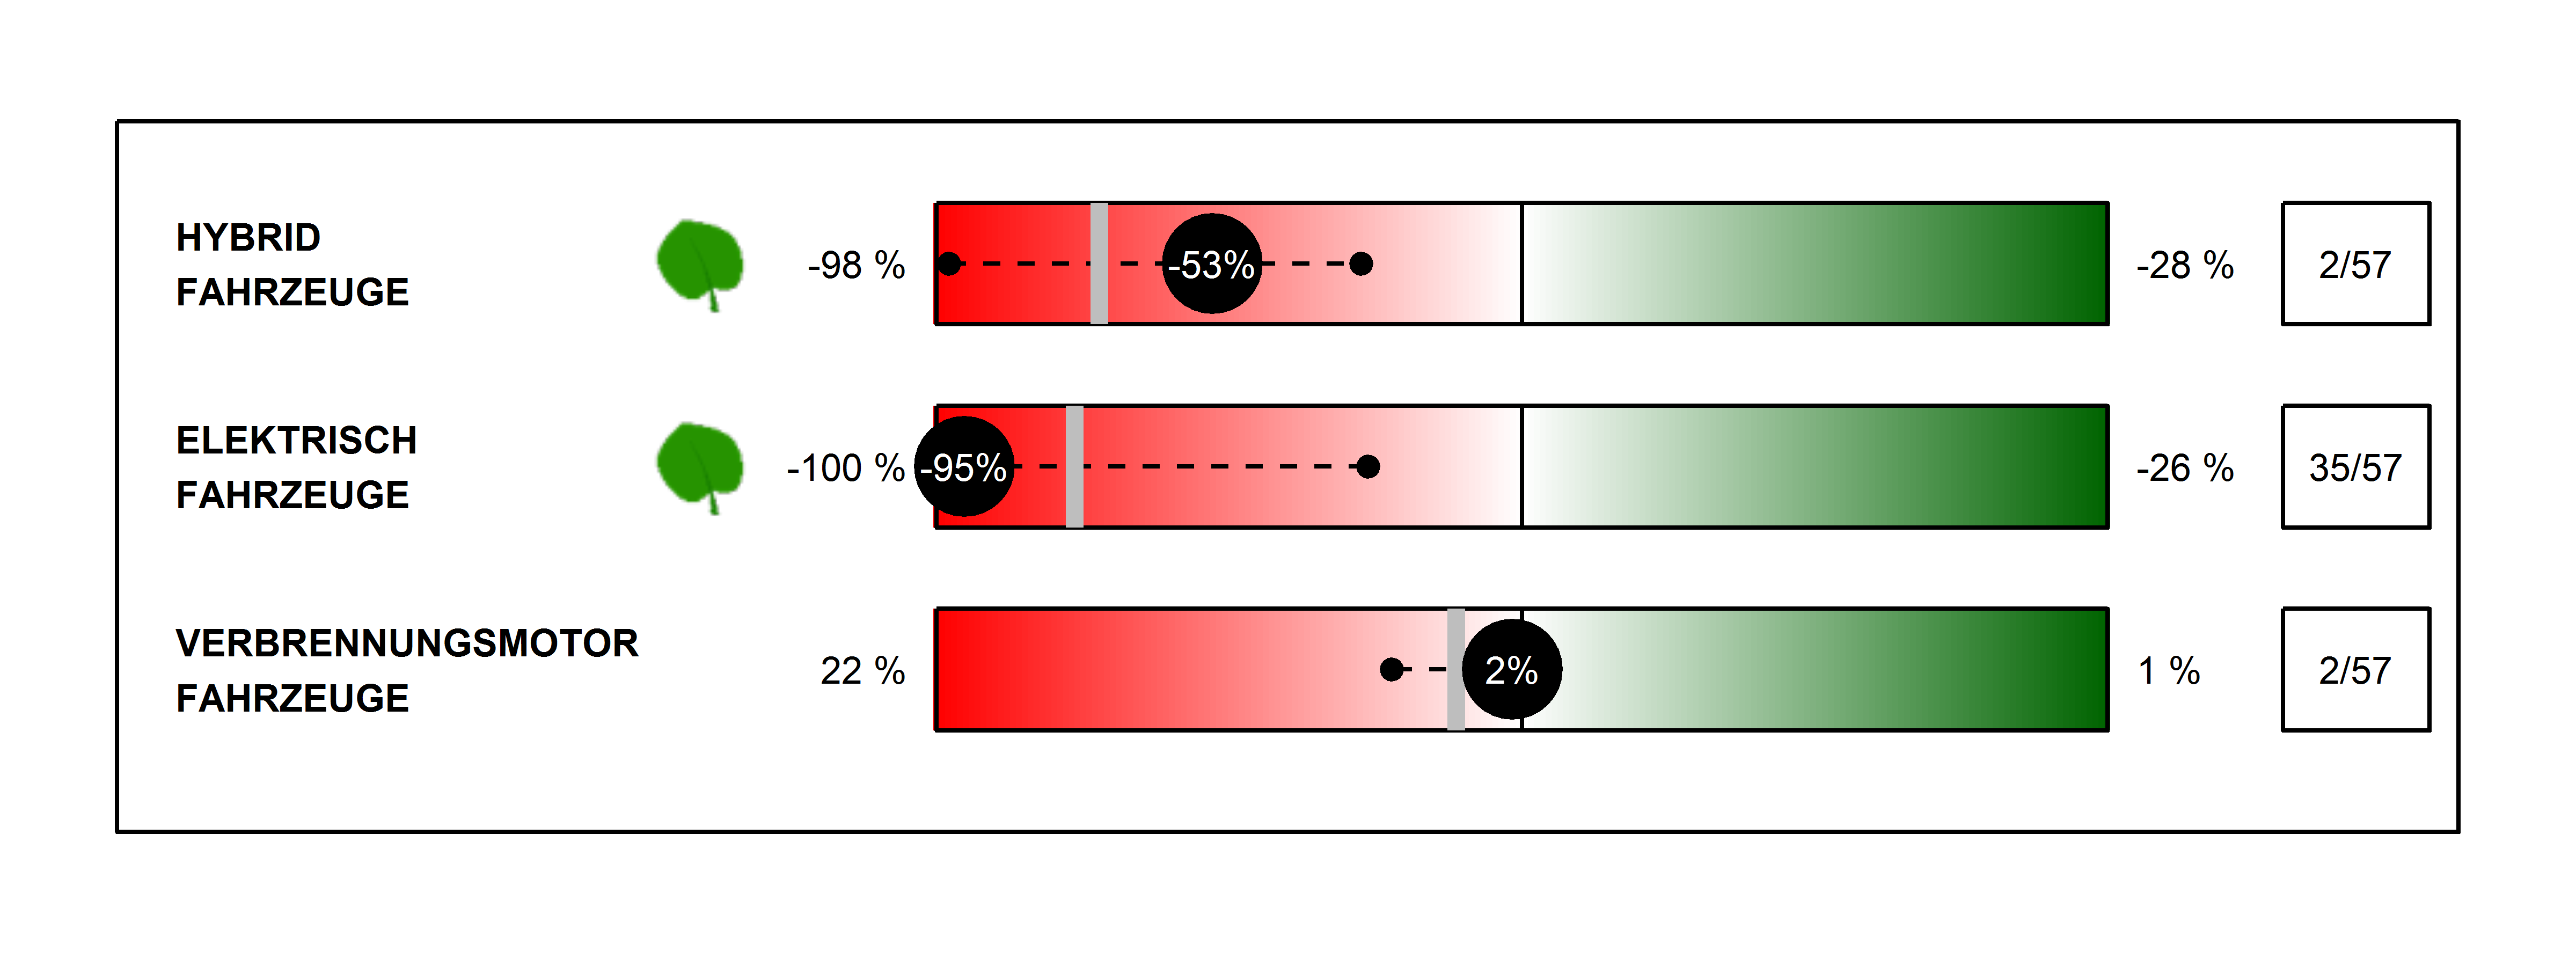
\includegraphics[trim = {0 0cm 0 0},width=1\linewidth]{SwissFigures/Fig20}
			\textbf{CaptionWeight TechElectric CBCaptionElectric}
		\end{minipage}		
		
		{\centering\includegraphics[trim={0 .3cm 0 0.3cm},clip,width=.6\linewidth]{ReportGraphics/LineChartLegend_Languagechoose}\par}
}}

ContentTech2

\fbox{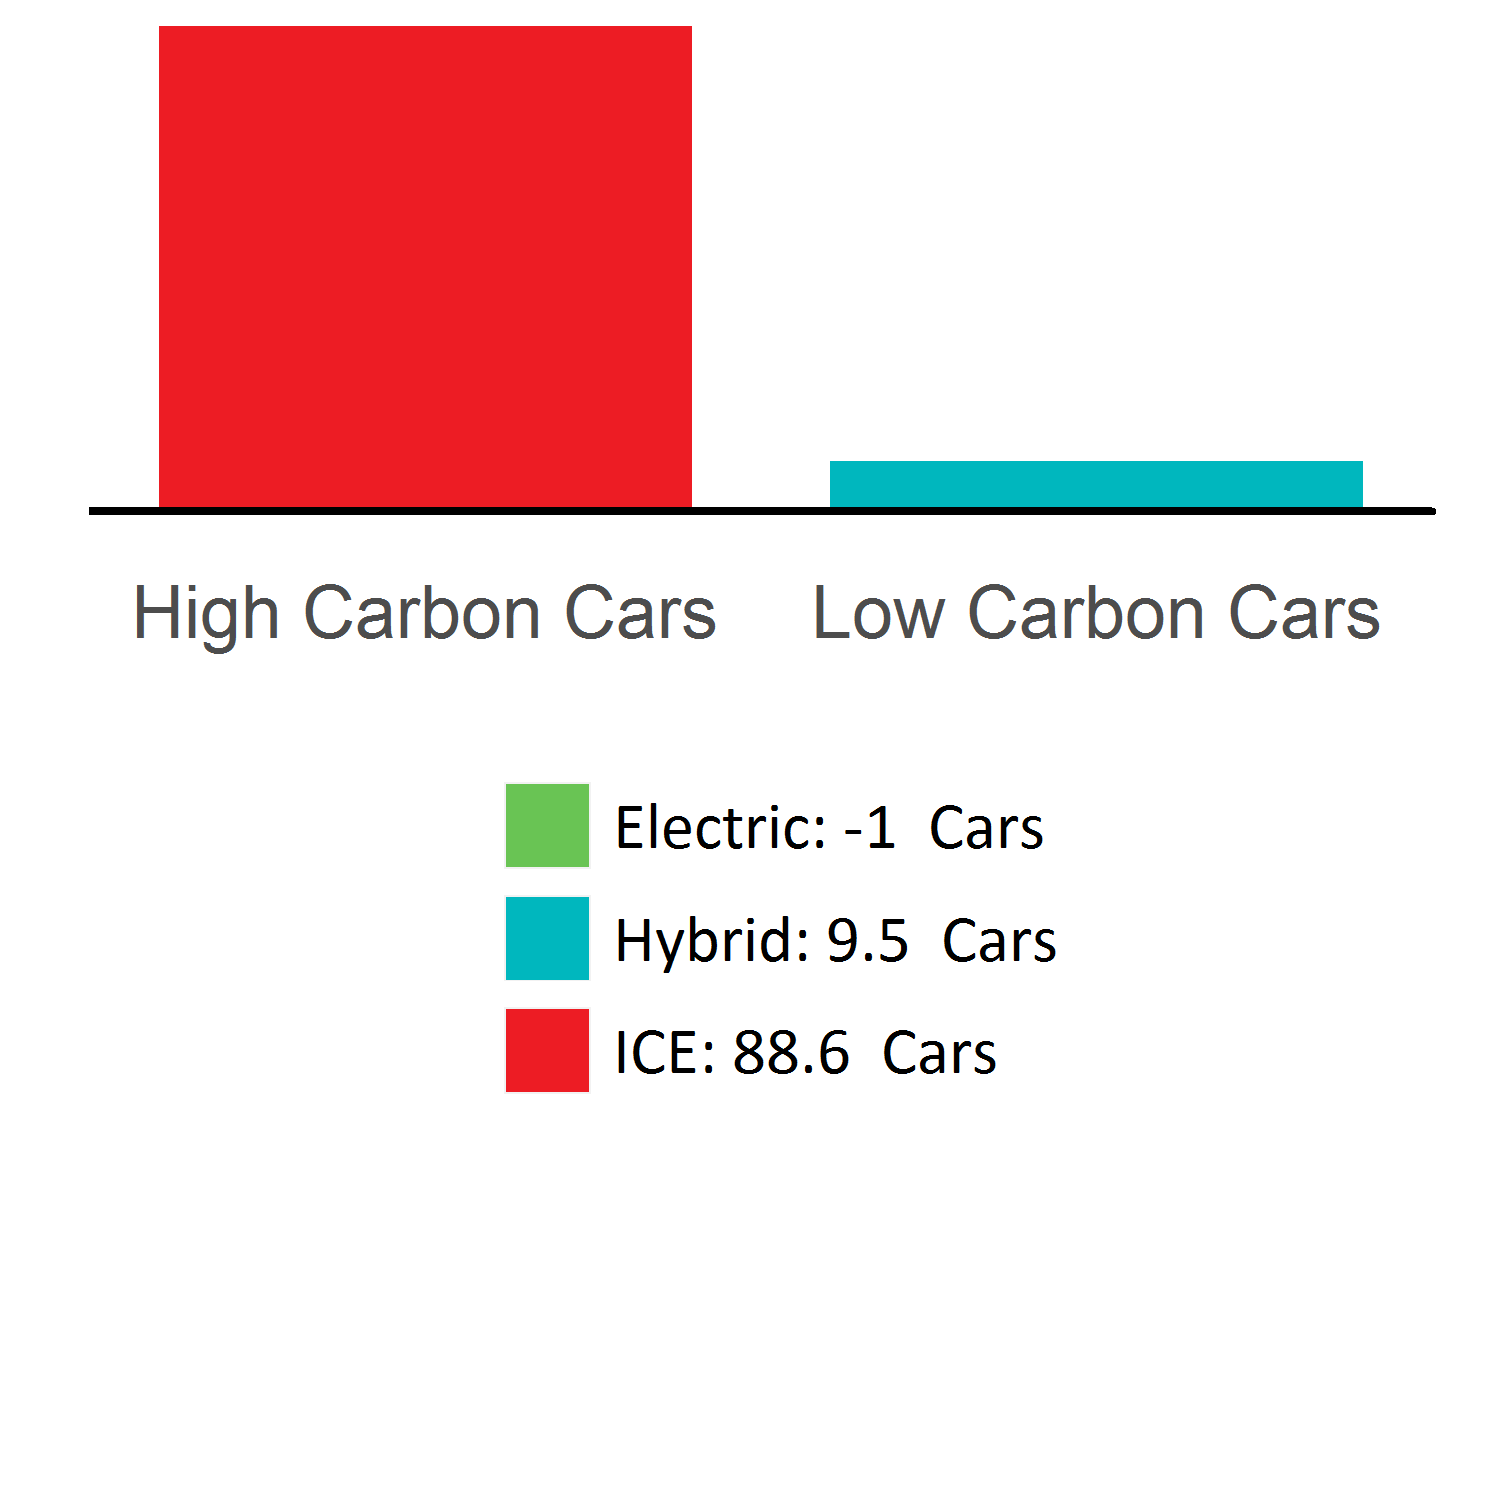
\includegraphics[trim={0 0.9cm 0 0.8cm},clip,width=1\linewidth]{SwissFigures/Fig22}}

\textit{\small SourceAuto}

\newpage %AutomotiveCBE CBPageE
\section*{P14} 		% Ranking EQ EQPageS
\PageHeading{HeadingP14}

ContentP14

\fcolorbox{black}{white}{ 
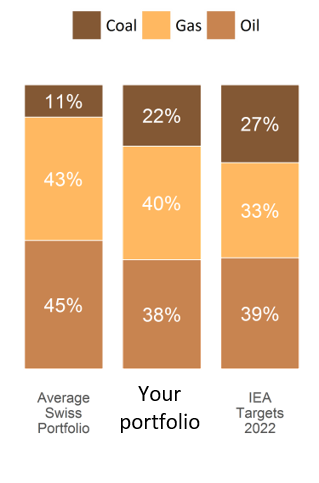
\includegraphics[trim={0 0.8cm 0 0.8cm},clip,width=1\linewidth]{SwissFigures/Fig33}}

\textit{\small SourceAll}

\newpage % EQPageE
\section*{P15} 		% Ranking CB CBPageS
\PageHeading{HeadingP15}

ContentP15

\fcolorbox{black}{white}{ 
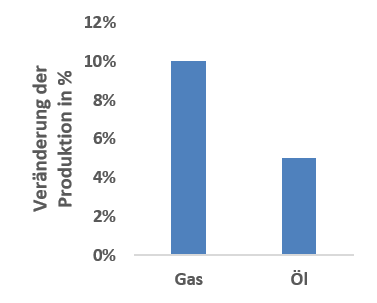
\includegraphics[trim={0 .8cm 0 0.8cm},clip,width=1\linewidth]{SwissFigures/Fig34}}

\textit{\small SourceAll}

\newpage % CBPageE
\section*{P16} 		% FundCheckS 
\PageHeading{HeadingP16}

ContentP16

\fcolorbox{black}{white}{ 
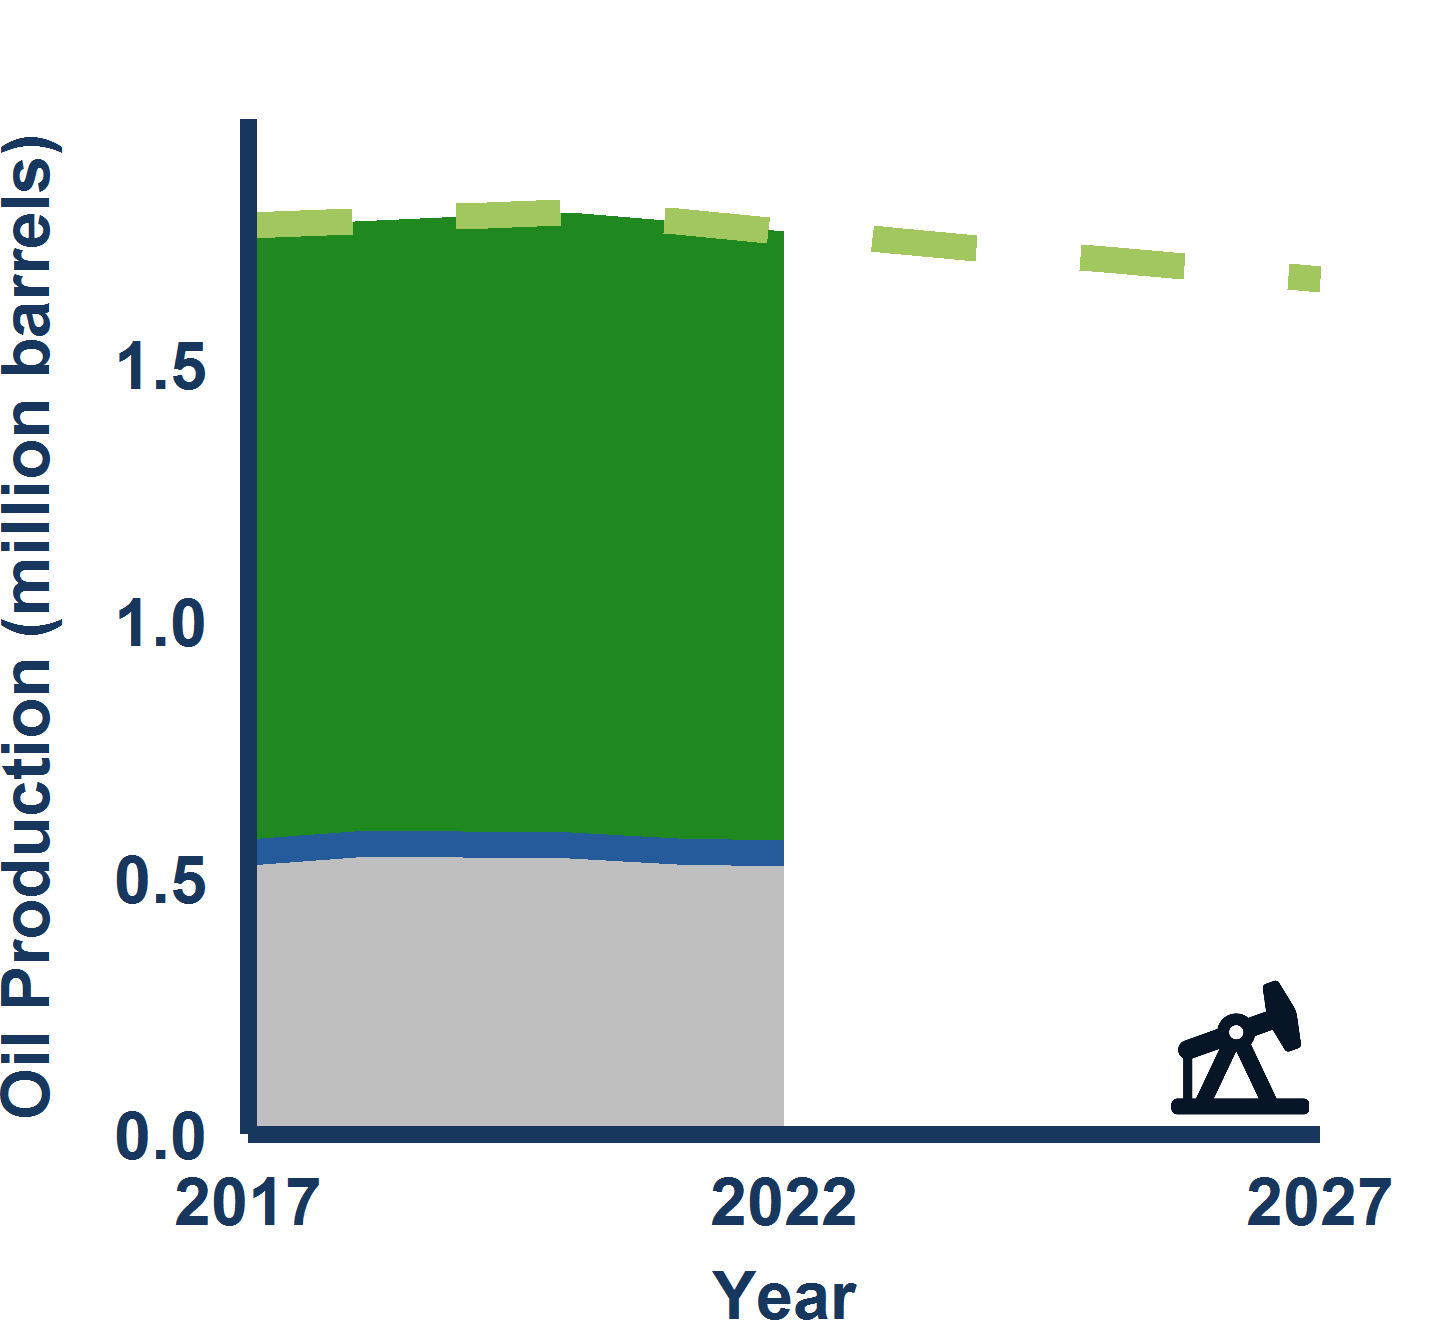
\includegraphics[trim={0 0cm 0 0cm},clip,width=1\linewidth]{SwissFigures/Fig35}}

\textit{\small SourceFunds}

\newpage	% FundCheckE 
\section*{P17} 		% OtherSectorsMaterialS
\PageHeading{HeadingP17} 

ContentP17

{\centering
\begin{minipage}[t]{.44\textwidth} %Cement
	\fcolorbox{black}{white}{ 
		\parbox{1\linewidth}{
			\textbf{CaptionP17a}
			
			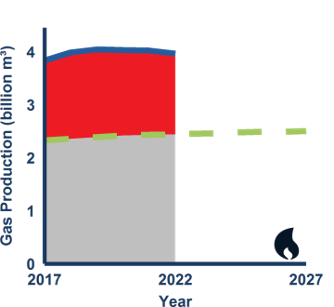
\includegraphics[width=.9\linewidth]{SwissFigures/Fig36}}
	}
\end{minipage}
\hspace{.5cm}
\begin{minipage}[t]{.44\textwidth}  %Steel
	\fcolorbox{black}{white}{ 
		\parbox{1\linewidth}{
			\textbf{CaptionP17b}
			
			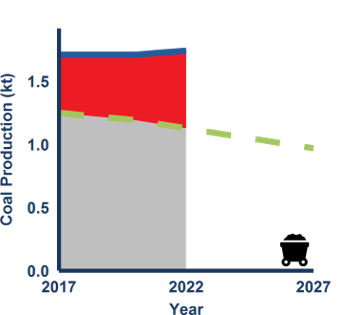
\includegraphics[width=.9\linewidth]{SwissFigures/Fig37}}
	}
\end{minipage}}

\includegraphics[width=1\linewidth]{ReportGraphics/P16_OtherSectorsLegend_Languagechoose}

\textit{\small SourceCement}

\newpage			% OtherSectorsMaterialE
\section*{P18} 		% OtherSectorsTransportS
\PageHeading{HeadingP18} 

ContentP18

{\centering
	\begin{minipage}[t]{.45\textwidth} %Aviation
		\fcolorbox{black}{white}{ 
			\parbox{1\linewidth}{
				\textbf{CaptionP18a}
				
				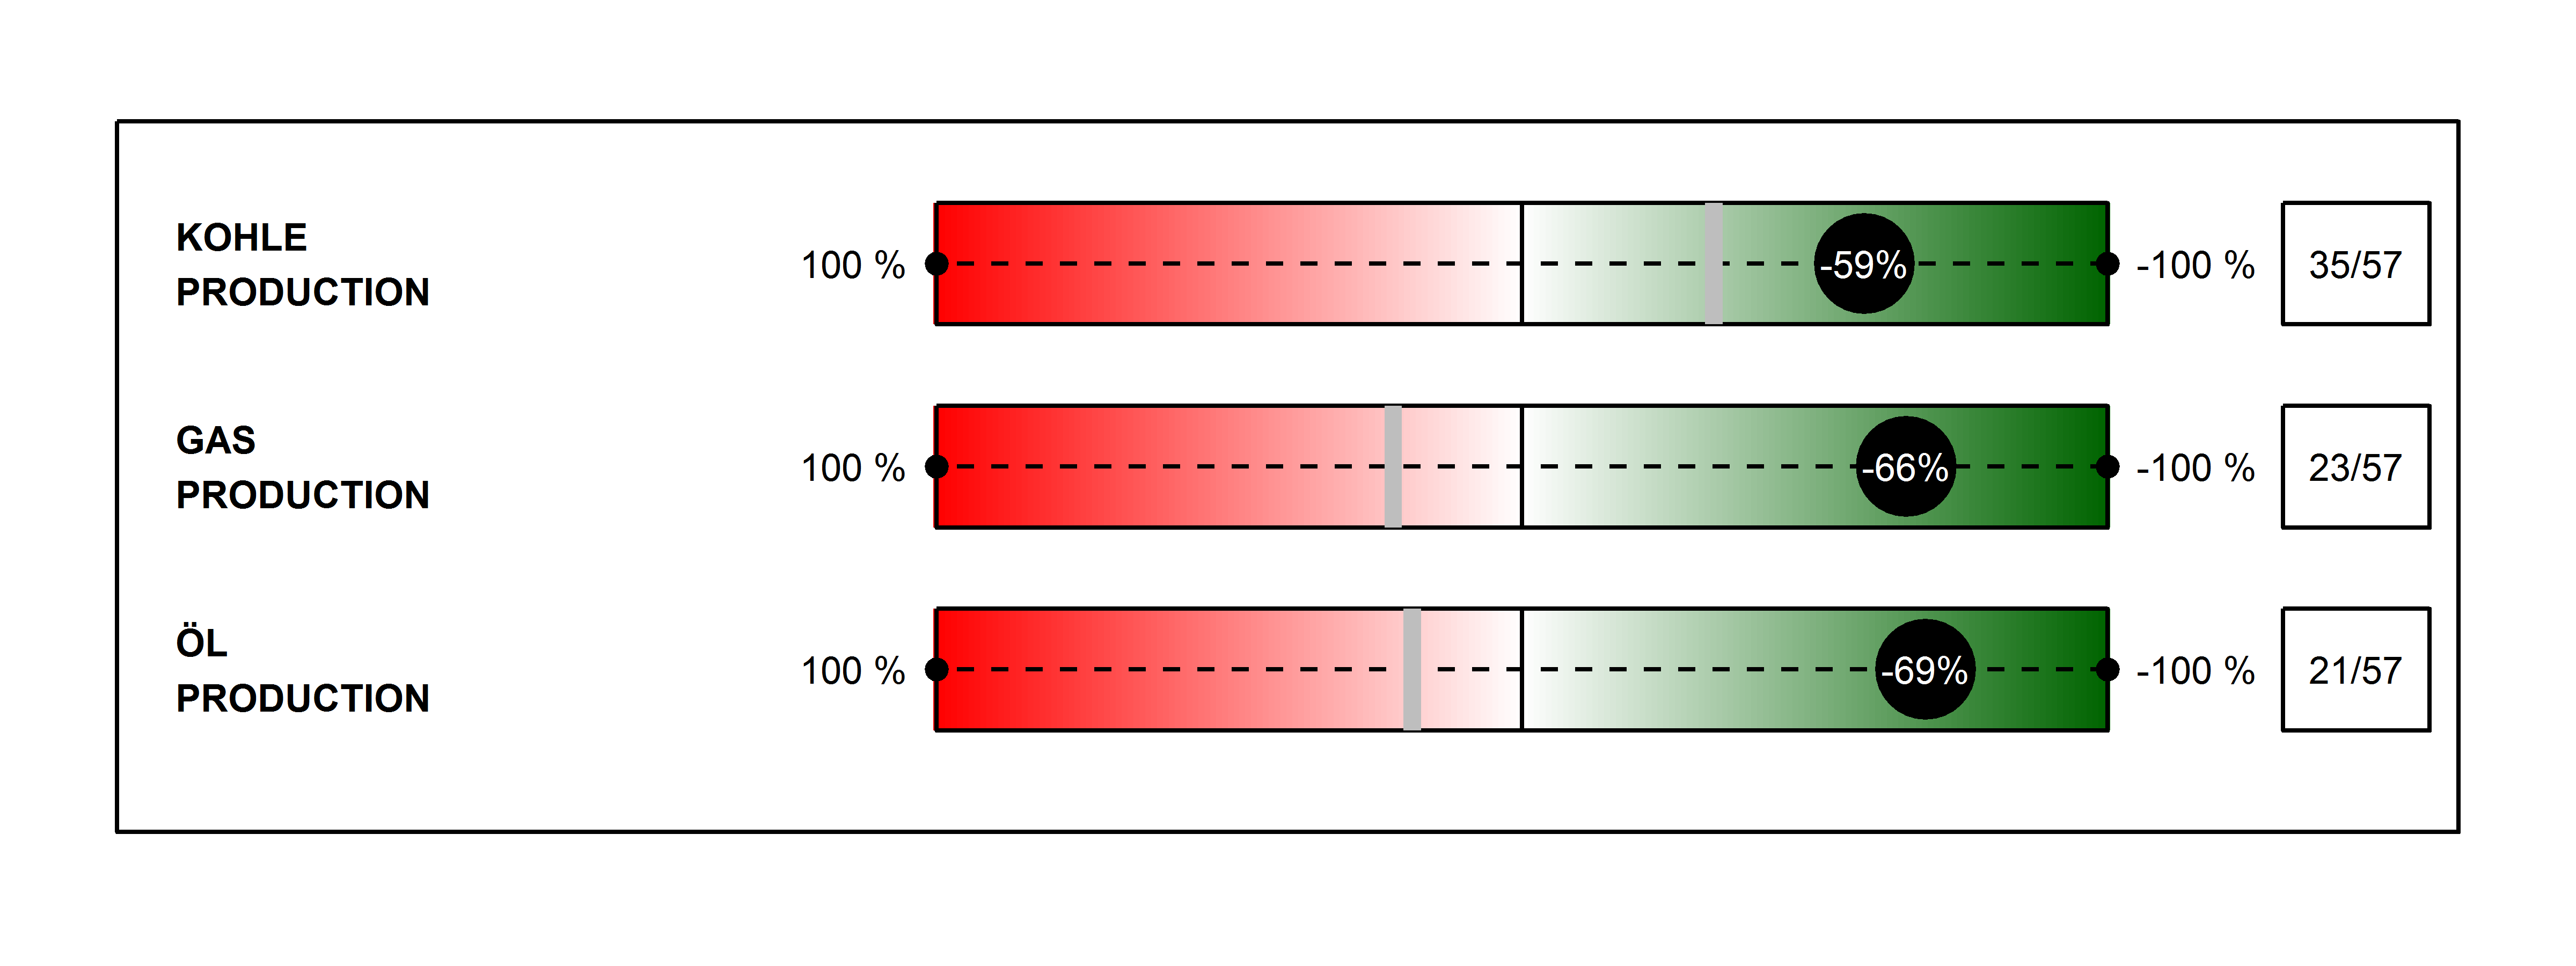
\includegraphics[width=.9\linewidth]{SwissFigures/Fig38}}
		}
	\end{minipage}
	\hspace{.5cm}
	\begin{minipage}[t]{.45\textwidth} %Shipping
		\fcolorbox{black}{white}{ 
			\parbox{1\linewidth}{
				\textbf{CaptionP18b}
				
				\includegraphics[width=.9\linewidth]{SwissFigures/Fig39}}
		}
	\end{minipage}
}

\includegraphics[width=1\linewidth]{ReportGraphics/P17_OtherSectorsLegend_Languagechoose}

\textit{\small SourceTransport}

\newpage 		% OtherSectorsTransportE 
\section*{P19} % 3rd Section
\thispagestyle{empty}
\vspace{17cm}
\SectionHeading{Section03:}{SectionTitle03}



\newpage
\singlespacing
\normalfont
\pagecolor{white}
\color{black}

\section*{P20}
\PageHeading{HeadingP20}

ContentP20a

\begin{minipage}[t]{.48\textwidth}

\begin{tcolorbox}[width=1\linewidth, arc=0pt,colback=2dblue]
	\centering
	\textcolor{white}{\large\bfseries CaptionP20a}	
\end{tcolorbox}

ContentP20b

\end{minipage}
\hspace{.5cm}
\begin{minipage}[t]{.48\textwidth}
\begin{tcolorbox}[width=1\linewidth, arc=0pt,colback=2dblue]
	\centering
\textcolor{white}{\large\bfseries CaptionP20b}	
\end{tcolorbox}

ContentP20c

\end{minipage}


\newpage

\section*{P21}
\PageHeading{HeadingP21}

ContentP21a

%\begin{enumerate}
%	\item \textbf{HeadP21i1} ListP21i1 
%	
%	\item \textbf{HeadP21i2} ListP21i2
%	
%	\item \textbf{HeadP21i3} ListP21i3
%
%	\item \textbf{HeadP21i4} ListP21i4
%\end{enumerate}
%
%ContentP21b

\newpage
%\section*{P22} % RISK SECTION
%\PageHeading{HeadingP22}
%\includegraphics[width=1\linewidth, trim={0 3cm 0 0 },clip]{SwissFigures/Fig43}
%\newpage
\section*{P23}
\PageHeading{HeadingP23}

ContentP23

%CaptionP23a
%
%{\centering\includegraphics[width=.8\linewidth]{SwissFigures/Fig41}\par}
%\vspace{-3.8cm}
%
\textbf{CaptionP23b} CaptionP23c
\vspace{-0.8cm}

\includegraphics[width=1\linewidth]{SwissFigures/Fig43}
\textit{\small SourcePowerFF}
\newpage
\section*{P24}
\PageHeading{HeadingP24}

\textbf{CaptionP24a} CaptionP24b
 \vspace{-1cm}
 
{\centering\includegraphics[width=1\linewidth,trim={0cm 0.2cm 0cm 0cm},clip]{SwissFigures/Fig44}\par}

\textit{\small SourceAuto} 

\textbf{CaptionP24c} CaptionP24d
\vspace{-.8cm}

{\centering\includegraphics[width=1\linewidth,trim={0cm 0cm 0cm .2cm},clip]{SwissFigures/Fig46}\par}
\vspace{-.2cm}
\textit{\small SourceCarbonTracker}


\newpage
\section*{P25}
\PageHeading{HeadingP25}

ContentP25a

\begin{itemize}
	\item ListP25i1 

	\item ListP25i2

	\item ListP25i3
\end{itemize}

ContentP25b

\vspace{.2cm}
{\centering\includegraphics[width=.9\linewidth,trim={.2cm 0cm 0cm 1.6cm},clip]{ReportGraphics/FigureP22_Languagechoose}\par}

\textit{\small SourceFunds }

\newpage
\section*{P26}
\PageHeading{HeadingP26} 

\begin{wrapfigure}{r}{0.5\linewidth}
	\vspace{-.5cm}
	\textbf{\textit{CaptionP26a}}
	
	{\centering\includegraphics[width=1\linewidth,trim={0cm 1cm 0cm 1cm},clip]{ReportGraphics/FigureP23_Languagechoose}\par}
	
	\textit{\small SourceAuto}
	\vspace{-.9cm} %renewspacingworkaround
\end{wrapfigure}

ContentP26a

ContentP26b %RenewAddsOutS

\vspace{0cm}
\textbf{\textit{CaptionP26b}} 


\includegraphics[width=1\linewidth]{SwissFigures/Fig51}

\textit{\small{SourcePowerFF}} 
%RenewAddsOutE

\newpage
\section*{P27}
\PageHeading{HeadingP27a} 

ContentP27a

\textbf{HeadingP27b}

ContentP27b

\textbf{HeadingP27c} 

ContentP27c

\textbf{HeadingP27d} 

ContentP27d


\end{document}
